\documentclass{article}

% arXiv preprint: un-anonymizes via [preprint] option per NeurIPS 2026 handbook.
\usepackage[preprint]{neurips/neurips_2026}

\usepackage{amsmath, amssymb, amsthm}
\usepackage{graphicx}
\graphicspath{{../figures/}}
\usepackage{booktabs}
\usepackage{hyperref}
\usepackage{multirow}
\usepackage{array}
\usepackage{subcaption}
\usepackage{float}
\usepackage{xcolor}
\usepackage{bm}
\usepackage{tikz}
\usetikzlibrary{arrows.meta, positioning, fit, backgrounds, calc}
\usepackage{titlesec}

% Whitespace tightening (defaults LaTeX leaves alone; .sty already tightens captions/lists/math)
\setlength{\textfloatsep}{8pt plus 2pt minus 2pt}
\setlength{\intextsep}{8pt plus 2pt minus 2pt}
\setlength{\floatsep}{8pt plus 2pt minus 2pt}
\titlespacing*{\section}{0pt}{8pt plus 2pt minus 2pt}{4pt plus 1pt minus 1pt}
\titlespacing*{\subsection}{0pt}{6pt plus 1pt minus 1pt}{3pt plus 1pt minus 1pt}
\titlespacing*{\paragraph}{0pt}{4pt plus 1pt minus 1pt}{1em}

\newtheorem{definition}{Definition}
\newtheorem{proposition}{Proposition}
\newtheorem{assumption}{Assumption}

\DeclareMathOperator{\Var}{Var}
\DeclareMathOperator{\Cov}{Cov}
\DeclareMathOperator{\E}{E}

% NeurIPS-style answer macros (used in the paper checklist)
\providecommand{\answerYes}[1][]{\textcolor{blue}{[Yes]}#1}
\providecommand{\answerNo}[1][]{\textcolor{red}{[No]}#1}
\providecommand{\answerNA}[1][]{\textcolor{gray}{[NA]}#1}
\providecommand{\answerTODO}[1][]{\textcolor{orange}{[TODO]}#1}

% Public code repository (real GitHub URL for the preprint)
\newcommand{\codeurl}{\url{https://github.com/SolomonMg/totalevalerror}}
\newcommand{\codeurltext}{github.com/SolomonMg/totalevalerror}

\title{Hidden Measurement Error in LLM Pipelines Distorts Annotation, Evaluation, and Benchmarking}

\author{%
  Solomon Messing\thanks{Corresponding author.} \\
  Center for Social Media, AI, and Politics, New York University \\
  MLCommons \\
}

\begin{document}

\maketitle

\begin{abstract}
LLM evaluations drive which models get deployed, what safety standards get adopted, which research conclusions get published, and how projections of AI's labor-market impact get made. Yet standard confidence intervals ignore variability from judge model choice, model temperature, and prompt phrasing, producing under-coverage that worsens with more data. The omitted variance can shift results enough to reverse conclusions \citep{baumann2025llmhacking, huang2026dropping}; pipelines that fail to average over it leave the surface that ``benchmark hacking'' exploits \citep{singh2025leaderboard}. This paper decomposes LLM pipeline uncertainty into its sources, distinguishes variance that shrinks with more data from sensitivity to researcher design choices, and uses design-study projections to reduce total evaluation error (TEE). Across the demonstrations, naive standard errors are 40 - 60\% smaller than the TEE-corrected SE. Using Chatbot Arena data, we show naive 95\% CI coverage drops as $n$ grows while TEE-corrected coverage holds at 95\%, and TEE-guided pipelines restrict the benchmark gaming surface from 56 to 32 Elo ($K=27$), below the human-leaderboard baseline. We show further that a small pilot recovers honest CIs and projects which design changes most improve precision. Acting on those projections roughly halves MMLU estimation error against the answer key at equivalent cost, and raises per-match agreement with human votes by 7.9 percentage points on Chatbot Arena.
\end{abstract}

\section{Introduction}
\label{sec:intro}

LLM measurement pipelines introduce variance at multiple stages that traditional reporting norms ignore. Researchers who use LLMs for annotation, evaluation, or content moderation routinely do so with no assessment of prompt sensitivity, temperature dependence, or item-level heterogeneity \citep{pecher2026underspecification, barrie2025replication}. Benchmark scores likewise depend on prompt wording and scoring model choice, and this dependence is seldom measured (SI Appendix, Table~\ref{tab:current_practice}).\footnote{AlpacaEval and Chatbot Arena report item-sampling CIs; AILuminate uses a multi-judge evaluator ensemble; no benchmark decomposes prompt, temperature, or interaction variance. Full 13-benchmark survey in SI Appendix, Table~\ref{tab:current_practice}.} In all cases, unmeasured variation can create analogues to $p$-hacking \citep{simmons2011falsepositive, gelman2013garden} and overfitting \citep{recht2019imagenet} such that the results reflect measurement noise, not general phenomena.

At best, current practice reports confidence intervals (CIs) reflecting variation from repeated sampling at identical settings, ignoring prompt sensitivity, item heterogeneity, and their interactions. Figure \ref{fig:underestimation} presents simulation results showing that we should expect under-coverage to \emph{worsen} with more items, because omitted variance from prompt and judge choices does not shrink with~$N$.\footnote{Variance parameters estimated via REML under the framework introduced below; 1,000 simulation replicates per data point (SI Appendix, Section~\ref{si:underestimation_sim}).}

\begin{figure}[htbp]
\centering
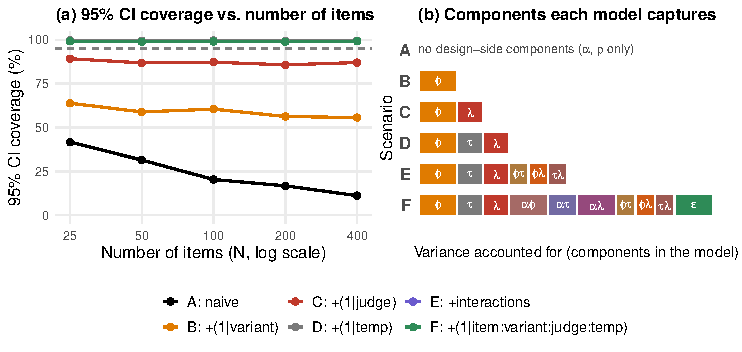
\includegraphics[width=0.9\linewidth]{fig_underestimation_slide_v2.pdf}
\caption{Naive confidence intervals fail because pipeline variance from prompt, judge, and temperature choice does not shrink with items ($N$). (a)~95\% CI coverage versus $N$ in six scenarios (A - F). (b)~Variance components each scenario accounts for. Scenario A is the naive estimate $\Phi^{-1}(0.975) \times s/\sqrt{N}$; B - F add variance parameters from the framework below, F including the item interactions and $\sigma^2_\epsilon$. D - F overlap near 99\% (E lies under F).%Scenarios: A, $\mathrm{SE}=s/\sqrt{N}$; B adds $V=3$ prompts and fits $(1\,|\,\text{item})+(1\,|\,\text{variant})$, capturing $\phi$. C adds $M=3$ judges and $(1\,|\,\text{judge})$, capturing $\lambda$. D adds $H=3$ temperatures and $(1\,|\,\text{temp})$, capturing $\tau$. E adds $(1\,|\,\text{variant:judge}) + (1\,|\,\text{variant:temp})$ for the pairwise interactions.DGP parameters rescaled for illustrative purposes.
}
\label{fig:underestimation}
\end{figure}

The problem is especially urgent in benchmarking, where unstable scores make rank-order differences between closely spaced models (or systems under test, SUT) uninterpretable for evaluators and give model developers exploitable degrees of freedom. On stable measurement, \citet{romanou2026brittlebench} show that semantics-preserving input perturbations explain near half of performance variance, minor reorderings of answer choices shift MMLU leaderboard rankings by up to 8~positions \citep{alzahrani2024benchmarks}, and on Chatbot Arena dropping just 0.003\% of human preferences is enough to flip the top-ranked model \citep{huang2026dropping}. With respect to exploitation, \citet{singh2025leaderboard} document best-of-$K$ leaderboard gaming in production, the mechanism Section~\ref{sec:gaming} quantifies.

Ignoring this variability can harm the scientific literature as well. One re-evaluation study found 31\% of hypotheses tested with LLM annotations yielded incorrect conclusions under LLM configuration variation (model, prompt, temperature, output mapping), and found malicious actors could reverse the sign of 68\% of statistically significant effects through adversarial configuration selection \citep{baumann2025llmhacking}. Other work has found that formatting choices alone produced a 76-point accuracy spread \citep{sclar2024sensitivity}, while infrastructure nondeterminism shifted results by up to nine percentage points even at temperature zero \citep{yuan2025numerical}.\footnote{$T = 0$ does not remove model uncertainty. Greedy decoding returns one deterministic path, but the token distribution keeps its entropy, and for chain-of-thought models early token choices compound along that path \citep{renze2024temperature}.}

\section{Related Work}

Several concurrent works address pieces of this problem, including variance decomposition \citep{haase2026withinmodel, wang2024measuring}, uncertainty quantification \citep{longjohn2025statistical}, sensitivity taxonomies \citep{romanou2026brittlebench}, meta-evaluation of benchmark reliability \citep{mcgregor2025benchrisk}, and tests of whether LLMs can replace human annotators \citep{calderon2025alttest}. \citet{camuffo2026variance} build a five-part variance taxonomy for LLM annotation and tie annotation variance to downstream bias. NIST AI 800-3 \citep{keller2026nist} fits a GLMM to benchmark data and separates benchmark accuracy from generalized accuracy as estimands. \citet{song2025gtheory} apply G-theory to writing assessment. \citet{dobriban2025statistical} note that a unified statistical methodology for evaluation ``remains to be developed'' (SI Appendix, Section~\ref{si:comparison}).

\section{Framework}
\label{sec:framework}

We call the framework \textit{Total Evaluation Error} (TEE, Figure~\ref{fig:pipeline}). TEE decomposes pipeline variance into components that include the first-order interactions, then projects from those components the standard error of any design a researcher might run. The projections are what let us calibrate CIs, allocate budget, and shrink the surface that benchmark gaming exploits. The name follows total survey error \citep{sen2019tedon, groves2010survey}, which treats every stage of a measurement pipeline as a source of error, and the framework draws on the text-as-data literature \citep{grimmer2013text}. %\footnote{``Total'' refers to accounting for items, prompts, judges, temperatures, replications and their interactions. It does not model every conceivable source of operational variation. For example, cross-layer interactions between the system under test and the judge are not captured by the current within-layer decomposition, though extensions are certainly possible.}. 

%combines crossed prompt, judge, and temperature random effects \textit{with their interactions} to more fully decompose the variance and allow for better calibrated CIs. It also provides projections that can be used by analysts and evaluators to reduce error and benchmark hacking vulnerability, by translating the decomposition into D-study allocations and gaming-surface bounds.  %TEE enables researchers to identify the dominant sources of pipeline uncertainty and benchmark builders to diagnose which design choices are most exploitable (SI Appendix, Table~\ref{tab:gaming}).

\subsection{Relation to Generalizability Theory}
\label{sec:gtheory}

TEE operationalizes generalizability theory (G-theory) for LLM pipelines \citep{cronbach1972dependability, brennan2001gtheory, shavelson1991gtheory, bayerl2007gtheory} and uses its standard estimators. Our contribution is the LLM-specific measurement design that makes prompts, temperatures, models, judges, scoring methods, and interactions such as item$\times$judge and prompt$\times$judge explicit sources of pipeline error, where today they are hidden implementation choices. Four links to G-theory carry the rest of the paper.

(1)~The universe of admissible observations here spans items, prompt phrasings, judge models, SUT models, decoding temperatures, replications, and scoring protocols. The object of measurement is the \emph{item}, the unit whose score the evaluation generalizes over. On MMLU an item is a benchmark question. On safety and Arena a judge scores model output, and an item is the fixed evaluation case, a user prompt plus the SUT response(s) being judged. The prompt variants that instruct the judge index a facet of their own.
(2)~We apply the random versus fixed distinction to LLM design choices. Facets we sample over (items, prompt variants, replications) contribute uncertainty that averaging shrinks. A model, temperature, or scoring protocol we hold fixed is a design feature, and its contribution belongs in a sensitivity analysis (Section~\ref{sec:dgp}).
(3)~A G-study diagnoses which facets and interactions dominate under the design actually run (Section~\ref{sec:gstudy}). A D-study projects which alternative design would reduce the target SE (Section~\ref{sec:dstudy}). We map those projections onto budget choices and test how far the rankings survive pilot-size limits and misspecification.
(4)~The scoring protocol produces the observed score, so it belongs to the measurement design. Estimated components change under binary or Likert judging versus Bradley-Terry pairwise scoring, and on the probability versus the logit scale (SI Appendix, Sections~\ref{si:scoring_comparison} and~\ref{si:glmm}).

Classical G-theory grew up where raters are scarce and expensive while items and occasions are cheap, so its D-studies mostly ask how many raters one can afford \citep{brennan2001gtheory}. LLM pipelines price every facet in the same unit. An extra judge, prompt variant, item, or replication adds API calls in proportion to the rest of the design, and none of them needs recruiting or training, so every facet competes for one budget and the D-study has to rank them. TEE measures reliability. Judge correctness and construct coverage are validity questions that need external data, and Sections~\ref{sec:safety} and~\ref{sec:limitations} say what to pair the decomposition with.

\begin{figure}[t!]
\centering
\resizebox{0.82\linewidth}{!}{%
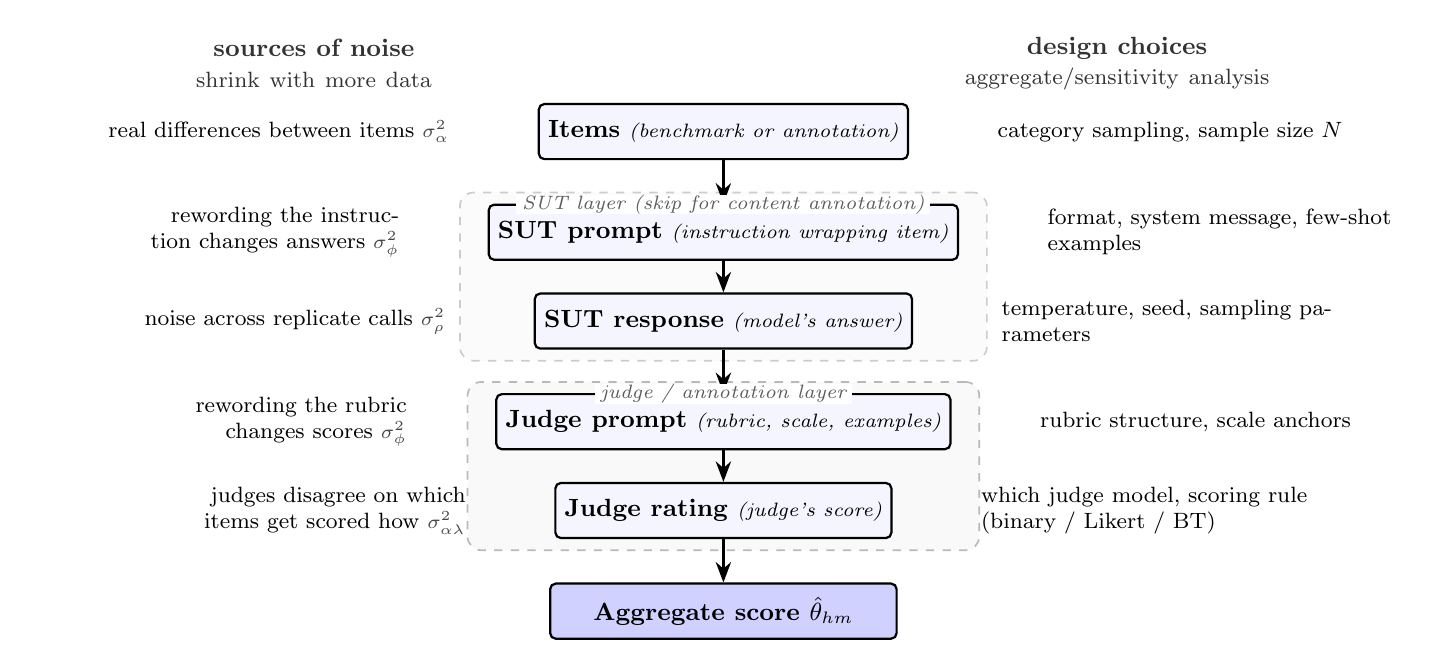
\begin{tikzpicture}[
    node distance=0.4cm and 1.6cm,
    box/.style    = {rectangle, draw, thick, rounded corners=2pt,
                     minimum width=4.0cm, minimum height=0.7cm,
                     align=center, font=\small, fill=blue!4},
    final/.style  = {box, fill=blue!18, font=\bfseries\small,
                     minimum width=4.4cm},
    layer/.style  = {draw=gray!55, dashed, semithick, rounded corners=5pt,
                     inner xsep=10pt, inner ysep=4pt, fill=gray!5},
    llabel/.style = {font=\scriptsize\itshape, text=gray!72!black,
                     fill=white, inner xsep=2pt, inner ysep=0pt},
    vleft/.style  = {font=\footnotesize, align=right, anchor=east,
                     text width=4.6cm},
    vright/.style = {font=\footnotesize, align=left,  anchor=west,
                     text width=4.6cm},
    arrow/.style  = {-{Stealth[length=2.6mm]}, thick},
    header/.style = {font=\small\bfseries, align=center,
                     text=gray!40!black, text width=4.6cm}
]

% ========= central pipeline =========
\node[box]                            (items)  {\textbf{Items} {\scriptsize\itshape(benchmark or annotation)}};
\node[box, below=0.55cm of items]     (sutpr)  {\textbf{SUT prompt} {\scriptsize\itshape(instruction wrapping item)}};
\node[box, below=of sutpr]            (sutres) {\textbf{SUT response} {\scriptsize\itshape(model's answer)}};
\node[box, below=0.55cm of sutres]    (jpr)    {\textbf{Judge prompt} {\scriptsize\itshape(rubric, scale, examples)}};
\node[box, below=of jpr]              (jres)   {\textbf{Judge rating} {\scriptsize\itshape(judge's score)}};
\node[final, below=0.55cm of jres]    (agg)    {Aggregate score $\hat{\theta}_{hm}$};

\draw[arrow] (items)  -- (sutpr);
\draw[arrow] (sutpr)  -- (sutres);
\draw[arrow] (sutres) -- (jpr);
\draw[arrow] (jpr)    -- (jres);
\draw[arrow] (jres)   -- (agg);

% ========= layer frames =========
% SUT layer drawn lighter to signal it is conditional on a benchmarking task.
\begin{scope}[on background layer]
  \node[layer, draw=gray!40, fill=gray!3,
        fit=(sutpr)(sutres)] (sutlayer) {};
  \node[layer, fit=(jpr)(jres)]      (jlayer)   {};
\end{scope}
\node[llabel, anchor=north] at ([yshift=-1pt]sutlayer.north)
   {SUT layer (skip for content annotation)};
\node[llabel, anchor=north] at ([yshift=-1pt]jlayer.north)
   {judge / annotation layer};

% ========= LEFT: random variance =========
\node[vleft] at ([xshift=-1.0cm]items.west)
    {real differences between items {\scriptsize\textcolor{gray!55!black}{$\sigma^{2}_{\alpha}$}}};
\node[vleft] at ([xshift=-1.0cm]sutpr.west)
    {rewording the instruction changes answers {\scriptsize\textcolor{gray!55!black}{$\sigma^{2}_{\phi}$}}};
\node[vleft] at ([xshift=-1.0cm]sutres.west)
    {noise across replicate calls {\scriptsize\textcolor{gray!55!black}{$\sigma^{2}_{\rho}$}}};
\node[vleft] at ([xshift=-1.0cm]jpr.west)
    {rewording the rubric changes scores {\scriptsize\textcolor{gray!55!black}{$\sigma^{2}_{\phi}$}}};
\node[vleft] at ([xshift=-1.0cm]jres.west)
    {judges disagree on which items get scored how {\scriptsize\textcolor{gray!55!black}{$\sigma^{2}_{\alpha\lambda}$}}};

% ========= RIGHT: design choices =========
\node[vright] at ([xshift=1.0cm]items.east)
    {category sampling, sample size $N$};
\node[vright] at ([xshift=1.0cm]sutpr.east)
    {format, system message, few-shot examples};
\node[vright] at ([xshift=1.0cm]sutres.east)
    {temperature, seed, sampling parameters};
\node[vright] at ([xshift=1.0cm]jpr.east)
    {rubric structure, scale anchors};
\node[vright] at ([xshift=1.0cm]jres.east)
    {which judge model, scoring rule (binary / Likert / BT)};

% ========= column headers =========
\node[header] at ([xshift=-5.2cm,yshift=0.5cm]items.north)
    {sources of noise\\{\normalfont\footnotesize shrink with more data}};
\node[header] at ([xshift=5cm,yshift=0.5cm]items.north)
    {design choices\\{\normalfont\footnotesize aggregate/sensitivity analysis}};
\end{tikzpicture}}%

\caption{TEE separates aggregation-reducible noise from design-choice sensitivity at every pipeline stage. %Each variance component on the left shrinks with more items, prompts, or replications within a chosen design. Each design choice on the right is fixed within a design but its contribution shrinks across designs (averaging over multiple judges, temperatures, or scoring rules); when no aggregation occurs, the contribution should be reported as sensitivity. 
For content-annotation tasks (e.g., labeling social media posts) the SUT layer is omitted.}
\label{fig:pipeline}
\end{figure}
% \clearpage


Figure~\ref{fig:safety_combined}(a) illustrates the TEE decomposition. Three LLM judges \citep{zheng2023llmjudge} classify 141 safety items from the AILuminate benchmark. Judge design sensitivity contributes 43.8\% of the variance with item$\times$judge adding another 16.7\%. On the other hand, prompt wording contributes less than 0.5\%. In this example, investing in additional judges has higher returns to variance reduction than better prompts or additional benchmark items.

\subsection{Data-Generating Process}
\label{sec:dgp}

An LLM measurement pipeline produces a scored output $Y_{ivhm}^{(r)}$ depending on five factors: item~$i$ ($i = 1, \ldots, N$), prompt variant~$v$ ($v = 1, \ldots, V$), temperature~$h$ ($h = 1, \ldots, H$), model~$m$ (a judge at the judge layer, a SUT at the SUT layer), and replication~$r$ ($r = 1, \ldots, R$). A replication is a repeated API call with identical inputs. The framework specifies the linear mixed model:
\begin{equation}
\label{eq:dgp}
\begin{split}
Y_{ivhm}^{(r)} = \mu + \alpha_i + \phi_v + \tau_h + \lambda_m 
 + (\alpha\phi)_{iv} + (\alpha\tau)_{ih} + (\phi\tau)_{vh} 
 + (\alpha\lambda)_{im} + (\phi\lambda)_{vm} \\
 + \epsilon_{ivhm} + \rho_{ivhm}^{(r)}
\end{split}
\end{equation}
where $\mu$ is the grand mean, $\alpha_i$ is the item random effect, $\phi_v$ the prompt variant random effect, $\tau_h$ the temperature fixed effect, $\lambda_m$ the model fixed effect, the five parenthesized interaction terms are two-way interaction random effects, $\epsilon_{ivhm} \sim N(0, \sigma^2_\epsilon)$ captures cell-level error from unmodeled higher-order interactions, and $\rho_{ivhm}^{(r)} \sim N(0, \sigma^2_\rho)$ captures within-cell replicate noise. %$\epsilon_{ivhm}$ is constant within a cell, $\rho_{ivhm}^{(r)}$ varies by replication within a cell. %The cell-level term $\sigma^2_\epsilon$ does not shrink with replications $R$; only items, prompts, judges, and other facets indexing the cell can reduce it.

We treat items and prompt variants as \emph{random} because we wish to get an estimand over all items and prompts that might have been drawn, so we average over them. On the other hand, we treat temperature and model as \emph{fixed} because we purposefully assembled the judge panel and do not wish to generalize to some model population, and similarly we consider temperatures as analogous to a ``dose'' rather than something to be sampled. Temperature also has nonlinear, non-additive effects on output variance \citep{renze2024temperature, li2025hotcold} (SI Appendix, Section~\ref{si:temperature}). %Some LLM-as-judge applications may want to characterize variance across a population of judge models, for example to bound how rankings shift under arbitrary judge swap. We still treat model as fixed because exchangeability across typical judge panels is implausible (different model families, sizes, training distributions) and 3 - 4 judges is too few to estimate a between-model variance with usable precision; the design-sensitivity index instead summarizes spread across the specific chosen levels. 
% Averaging over an $M$-judge panel reduces the model contribution to the grand mean as $\sigma^2_\lambda/M$ (Eq.~\ref{eq:dstudy_multi}), which the empirical demonstrations rely on. 

\subsection{G-Study: Estimating the Variance Components}
\label{sec:gstudy}
The G-study is the factorial we actually run, and its output is one variance component per facet and interaction under that observed design. Three assumptions hold the decomposition together. The first is exchangeability. Any repeated call at the same settings could stand in for any other, and no prompt variant is systematically better than the rest. That is what makes prompts and replications draws from a population, so their contributions shrink as a design adds variants or repeated calls. A prompt that reliably beats its alternatives is a design choice, and adding variants would only dilute it. The second is additivity up to two-way interactions. Each variance component then belongs to one or two facets, and averaging over them divides its contribution by their counts. Higher-order terms land in the residual, which does no harm so long as they stay small. The third is that random effects are independent and normally distributed. Independence lets the total variance equal the sum of its parts. If the difficult items were also the prompt-sensitive ones, a cross term would appear that no facet owns. Normality does less work. It supplies the likelihood and the 1.96 in the confidence interval, and the variance estimates stay consistent without it \citep{jiang1996reml}. We state each assumption formally in SI Appendix, Section~\ref{si:framework}, and test how D-study projections hold up when each is violated in Section~\ref{si:simulations}.

Which variants are admissible is therefore a construct question, and we settle it with a screen that never sees scores \citep{cronbach1972dependability, groves2010survey, mizrahi2024multiprompt, sclar2024sensitivity, barrie2024pss}. We anchor on the original prompt and require each candidate to preserve the task or rubric, the inserted content, the answer format, and the reasoning and scoring mode. A deterministic check rejects candidates that drop an input placeholder or the answer-format instruction. An independent screener model, never used as a judge, then rates construct equivalence from 1 to 5, and we reject anything below 4. On safety and MMLU the decoys score 1.0 and 2.5, and every retained variant scores 4 or 5. Applied retroactively, the deterministic check flags one MMLU variant that the screener had passed, and we drop it (Section~\ref{sec:mmlu}). We then pick diverse admissible variants and report how the estimates move with breadth. Widening from strict paraphrase to the framing variants raises the MMLU prompt-attributable share of per-observation G-study variance from 2.1\% to 7.3\%, and a broader hand-authored set reaches 20.6\%, so we do not claim coverage saturation there. The safety share holds at 1.3\% across narrow, broad-wording, and broad-framing sets (SI Appendix, Section~\ref{si:prompt_admissibility}). These per-observation shares are a different quantity from the $\Var(\hat\theta)$ shares reported in Section~\ref{sec:empirical}.

At fixed temperature $h$ and model $m$, the observation-level variance decomposes as:
\begin{equation}
\label{eq:tle}
\begin{split}
\Var(Y \mid h, m) = \sigma^2_\alpha + \sigma^2_\phi + \sigma^2_{\alpha\phi} + \sigma^2_{\alpha\tau} \\
+ \sigma^2_{\phi\tau} + \sigma^2_{\alpha\lambda} + \sigma^2_{\phi\lambda} + \sigma^2_\epsilon + \sigma^2_\rho
\end{split}
\end{equation}
While the decomposition conditions on the temperature and model main effects ($\tau_h$ and $\lambda_m$), the interaction terms remain because they are variance components of random effects. When averaging over $M$ models, a design-sensitivity term $\sigma^2_\lambda = \frac{1}{M}\sum_m(\lambda_m - \bar{\lambda})^2$ is added. The same is true for averaging over multiple temperatures. Equation~\ref{eq:dgp} omits the temperature$\times$model interaction. A design that averages over both factors also adds a term for their interaction, $\sigma^2_{\tau\lambda}$ (SI Appendix, Section~\ref{si:framework}).

In practice the G-study is a single \texttt{lmer} call \citep{bates2015lme4}. Fixed factors enter as covariates, \texttt{temperature + model}, and every random facet or interaction enters as its own term, for example \texttt{(1|item) + (1|prompt\_variant) + (1|item:model)}. REML \citep{jiang1996reml} returns one variance estimate per term, and those estimates are the $\sigma^2$ components in Equation~\ref{eq:tle}. The D-study below divides each component by the number of levels of its facets that a proposed design averages over. The full formula, pilot-design thresholds, and bootstrap-CI guidance for small facet counts are in SI Appendix, Sections~\ref{si:estimation} and~\ref{si:checklist}.

%Random components (item, prompt variant, replication) shrink by aggregation within a chosen design; fixed-effect contributions (temperature, model, scoring method) shrink only by aggregating across designs, and otherwise should be reported as sensitivity alongside the point estimate \citep{steegen2016multiverse}.

\subsection{D-Study: Projecting Precision Under Alternative Designs}
\label{sec:dstudy}

The G-study reports which facets dominate under the design we ran. A D-study takes the estimated variance components and projects the variance of the grand mean $\hat{\theta}$ under any design a researcher might run. Following G-theory, primes mark the proposed design ($N'$ items, $V'$ prompt variants, $R'$ replications) and unprimed letters the estimation design (the G-study). Each component enters the projection divided by the number of levels the proposed design averages it over. Item heterogeneity is divided by $N'$, prompt sensitivity by $V'$, and judge sensitivity by the panel size $M$. Each interaction is divided by the product of the counts for the facets it spans, cell-level error by $N'V'M$, and replicate noise by $N'V'MR'$. The formula treats items as draws from a larger population. When a benchmark's fixed item set is itself the target, the $\sigma^2_\alpha / N'$ term drops out.

The item$\times$judge and prompt$\times$judge terms, $\sigma^2_{\alpha\lambda}$ and $\sigma^2_{\phi\lambda}$, are identifiable only when the estimation design crosses $M$ models; with a single model they fold into $\sigma^2_\alpha$ and $\sigma^2_\phi$ (SI Appendix, Section~\ref{si:framework}).\footnote{When items belong to categories, as in the demonstrations here, $\sigma^2_\alpha = \sigma^2_\kappa + \sigma^2_\delta$ splits item heterogeneity into between-category and within-category parts. Sampled categories would add a $\sigma^2_\kappa / C$ term. The categories here are fixed (specific hazard types, ideology dimensions, MMLU subjects), so $\sigma^2_\kappa$ stays inside $\sigma^2_\alpha / N'$.} The cell-level and replicate-noise variances are estimated per model and averaged over the panel, $\bar{\sigma}^2_\epsilon = \frac{1}{M}\sum_m \sigma^2_{\epsilon,m}$ and $\bar{\sigma}^2_\rho = \frac{1}{M}\sum_m \sigma^2_{\rho,m}$. At fixed temperature, the projected variance is

\begin{equation}
\label{eq:dstudy_multi}
\begin{split}
\Var(\hat{\theta}_h) = \frac{\sigma^2_\alpha}{N'} + \frac{\sigma^2_\phi}{V'} + \frac{\sigma^2_\lambda}{M} + \frac{\sigma^2_{\alpha\phi}}{N'V'} + \frac{\sigma^2_{\alpha\tau}}{N'} + \frac{\sigma^2_{\phi\tau}}{V'} %\\
+ \frac{\sigma^2_{\alpha\lambda}}{N'M} + \frac{\sigma^2_{\phi\lambda}}{V'M} + \frac{\bar{\sigma}^2_\epsilon}{N'V'M} + \frac{\bar{\sigma}^2_\rho}{N'V'MR'}
\end{split}
\end{equation}
The D-study variance gives the standard error and 95\% CI: $\hat{\theta} \pm 1.96 \cdot \sqrt{\Var(\hat{\theta})}$, accounting for all identified pipeline variance. When facet counts are small (e.g., $V = 3$), the result is moderate undercoverage (80 - 90\% instead of 95\%). Parametric bootstrap estimates restore nominal coverage at minimal additional cost (SI Appendix, Section~\ref{si:underestimation_sim}).

In Monte Carlo simulations (1,000 replicates), the D-study picks the correct top intervention in 98\% of runs under the default DGP. Under four assumption violations (correlated random effects, non-exchangeable prompts, non-normal scores, heterogeneous category interactions), projected variance stays within 8\% of the truth. A latent-ambiguity sweep that adds sparse three-way interactions keeps component-level bias below 9\% (SI Appendix, Sections~\ref{si:dstudy_validation} and~\ref{si:latent_ambiguity}).

\paragraph{Choosing facets and judges.}
Do not cross everything. Pilot over the factors that actually vary in deployment, fit the decomposition, and spend where the D-study ranking shows non-trivial variance. In our demonstrations one or two factors dominated, usually judge choice, and temperature and extra replications rarely mattered. Sampling parameters such as top-$p$ or top-$k$ enter exactly as temperature does. Direct versus chain-of-thought prompting, output format, and reasoning mode can change the construct itself, so model them as separate factors unless they pass the construct-equivalence screen of Section~\ref{sec:gstudy}. For judges, begin with a plausible and diverse panel and run a small crossed pilot. Judge marginals and leave-one-judge-out refits then sort calibration offsets from boundary-case disagreement (Section~\ref{sec:safety}), and human labels settle the question when they exist. Different prompt or judge selections can change the recommendation, so TEE is a diagnostic for the pipeline in hand.


\section{Empirical Demonstrations}
\label{sec:empirical}

We apply the TEE decomposition across three empirical domains in the main text: binary safety classification (AILuminate), multiple-choice QA (MMLU), and pairwise model comparison validated against human votes (Chatbot Arena). On safety and Arena the model facet is the judge panel. On MMLU there is no judge, and the model facet is the SUT scored against the answer key (Section~\ref{sec:gtheory}). Section~\ref{sec:gaming} then quantifies the gaming surface single-configuration benchmarks expose. In the SI, we provide a political affinity annotation demonstration (Section~\ref{sec:propaganda}) with a 9-annotator human baseline, a Likert vs pairwise scoring comparison (Section~\ref{si:scoring_comparison}), and a pilot validation showing that a small sample recovers the qualitative D-study guidance of a 4.5$\times$ larger full run (Section~\ref{si:pilot}).

\subsection{Safety: Judge Disagreement Dominates}
\label{sec:safety}

We first illustrate the variance decomposition using AILuminate~v1.0 \citep{ghosh2025ailuminate}, a safety benchmark from MLCommons. The benchmark assesses whether LLM responses cross safety lines across 12 hazard categories (hate speech, self-harm, violent crime, etc.). Most items are unambiguously safe (94\% safe rate) and the variance concentrates on the 6\% of borderline cases where judges disagree about whether a refusal is adequate. We decompose the variance across judges, prompts, temperatures, items, and their interactions, based on 36 DEMO prompts (3 per category) crossed with responses from Claude Opus~4.5, GPT-5.1, DeepSeek Chat~v3.1, and Grok~4.1 Fast (141 items after dropping 3 SUT refusals), scored under 5~prompt variants $\times$ 3~temperatures $\times$ 3~judges $\times$ 8~replications $= 50,760$ calls.%\footnote{We model the binary outcome with a linear probability model \citep[LPM;][]{angristpischke2009} because D-study projection formulas require linear variance components.}

The G-study (Figure~\ref{fig:safety_combined}(a)) identifies judge design sensitivity as the dominant lever, contributing 43.8\% of $\Var(\hat{\theta})$ at the operational design ($N{=}141$, $V{=}5$, $M{=}3$, $H{=}3$, $R{=}8$). Item$\times$judge interaction adds another 16.7\%. Judge choice shifts the headline rate, and panel members disagree about which specific items are safe. Aggregating across the three judges in the panel cuts the safety SE by 38\% because the model design-sensitivity $\sigma^2_\lambda$ and the item$\times$judge interaction $\sigma^2_{\alpha\lambda}$ both shrink as $1/M$ when the projection averages over $M$ judges (Eq.~\ref{eq:dstudy_multi}). 

The three judge-related terms (judge design sensitivity, item$\times$judge, prompt$\times$judge) sum to 73\% of $\Var(\hat{\theta})$. To check that no single judge produces this, we refit the model dropping each judge in turn, and the judge-related share stays between 68\% and 83\% (SI Appendix, Section~\ref{si:lojo}). The decomposition cannot say which judge is right. It does say where to look. A judge whose mean sits away from the rest of the panel calls for recalibration or removal, and items with large item$\times$judge disagreement are the boundary cases that need substantive review against human labels, known-answer items, or the hazard taxonomy.

\begin{figure}[htbp]
\centering
\begin{minipage}[t]{0.49\linewidth}
  \centering
  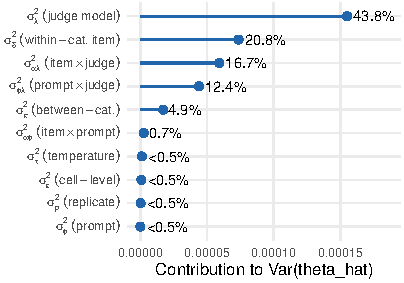
\includegraphics[width=\linewidth]{fig_intro_safety_decomposition.pdf}\\
  \footnotesize (a) Variance decomposition
\end{minipage}\hfill
\begin{minipage}[t]{0.49\linewidth}
  \centering
  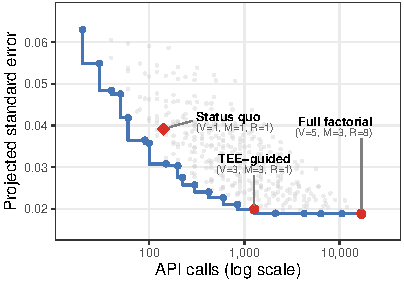
\includegraphics[width=\linewidth]{fig_cost_efficiency.pdf}\\
  \footnotesize (b) Cost-efficiency frontier
\end{minipage}
\caption{Safety decomposition (a) and cost-efficiency frontier (b) for AILuminate. Judge-model variance dominates the decomposition in (a). A TEE-guided design that aggregates over diverse judges captures most of the available SE reduction at modest cost (b).}
\label{fig:safety_combined}
\end{figure}


Within-category item heterogeneity contributes 20.8\% and prompt$\times$judge 12.4\%, with each remaining component below 5\%. Replicate noise $\sigma^2_\rho$ and cell-level error $\sigma^2_\epsilon$ are large components at the item level, but enter $\Var(\hat\theta)$ divided by $N'V'H'M'R'$ and $N'V'H'M'$ respectively, so each contributes less than 0.5\% to the variance of the mean. 
Temperature and prompt main effects contribute negligibly. \footnote{Three-way interaction terms (item$\times$prompt$\times$temperature, item$\times$temperature$\times$judge) are statistically significant but substantively negligible, supporting the two-way interaction specification.} 

%This is the across-design mode of aggregation introduced in Section~\ref{sec:framework}: judge model is treated as fixed in the DGP, but its contribution to the grand mean still shrinks when the design crosses multiple judges.

The D-study then projects precision under any proposed design (any new combination of $N'V'H'M'R'$, etc), enabling a cost-efficiency analysis. Figure~\ref{fig:safety_combined}(b) plots projected standard error against API cost for 360 candidate designs of the safety benchmark. The status quo (141 items, one prompt, one judge, no replication) sits well above the efficient frontier; at the same cost, frontier designs that trade items for judge diversity achieve 9\% lower SE. A TEE-guided estimation strategy (141 items, 3 prompts, 3 judges, no replication) cuts SE by 49\% at 9$\times$ the cost, while the full factorial (5 prompts, 3 judges, 8 replications) provides only an additional 5\% reduction at 120$\times$ the cost. The frontier flattens beyond approximately 1,000 calls, indicating steep diminishing returns to additional investment.



\subsection{MMLU: Item and Prompt Reallocation Roughly Halves Error}
\label{sec:mmlu}

Where LLM-as-judge is at the center of the safety demonstration, our MMLU benchmark analysis removes the judge layer entirely. MMLU (Massive Multitask Language Understanding) \citep{hendrycks2021mmlu} provides ground-truth labels for multiple-choice questions, letting us audit both pipeline accuracy and confidence-interval coverage against those answers. Three SUTs answered a 200-item pool under 4 prompt variants, 3 temperatures, and 8 replications (SI Appendix, Section~\ref{si:mmlu}).

The G-study (Figure~\ref{fig:mmlu_combined}(a)) attributes most of $\Var(\hat\theta)$ to which questions are sampled. Within-category item heterogeneity contributes 72.2\% and between-category heterogeneity 7.7\%, followed by item$\times$SUT (10.5\%) and SUT-model design sensitivity (6.7\%). Prompt wording barely matters on MMLU. The three prompt-related terms together hold 2.7\% of $\Var(\hat\theta)$, and accuracy moves only from 83.9\% to 85.3\% across the four prompt variants.\footnote{A fifth prompt variant gave the model only the question, the four options, and ``Answer:'', with no instruction to reply with a letter. With responses capped at 8 tokens, models often began explaining their reasoning and were cut off before choosing an option. Counting those cut-off responses as wrong would give the prompt-related terms 70\% of $\Var(\hat\theta)$. That 70\% measures a missing answer-format instruction. The admissibility check of Section~\ref{sec:gstudy} exists to catch exactly this, so we exclude that variant (SI Appendix, Section~\ref{si:mmlu_parsing}).} The logit-link refit agrees, with item heterogeneity leading at 71.4\% (SI Appendix, Section~\ref{si:glmm}).

The D-study then frames the evaluation as a budget-allocation problem, asking how to split a fixed total call budget across items ($N$), prompt variants ($V$), and replications ($R$). A 30-item pilot supplies the variance components, and the remaining 170 items form the pool. We compare three allocations, with the \emph{naive} allocation ($V\!=\!1$, $R\!=\!3$) replicating each call three times, the \emph{standard} allocation ($V\!=\!1$, $R\!=\!1$) skipping replication to fund more items, and the \emph{TEE-guided} allocation letting the D-study decide between adding items, prompts, or replications at each budget level. Because the two item terms hold 80\% of $\Var(\hat\theta)$, the D-study buys items first, so TEE and standard coincide until the pool runs out. Naive spends two-thirds of its calls on replications, which barely reduce error, and its RMSE is 1.6 to 2.4 times TEE's at every budget (Figure~\ref{fig:mmlu_combined}(b)). Once all 170 items are in use, standard stops improving, while TEE averages over prompt variants and roughly halves standard's RMSE at the largest budgets. TEE's 95\% CIs cover at 97 - 100\% throughout, and naive CIs under-cover only at the smallest budgets (91\% and 93\%).

\begin{figure}[htbp]
\centering
\begin{minipage}[t]{0.49\linewidth}
  \centering
  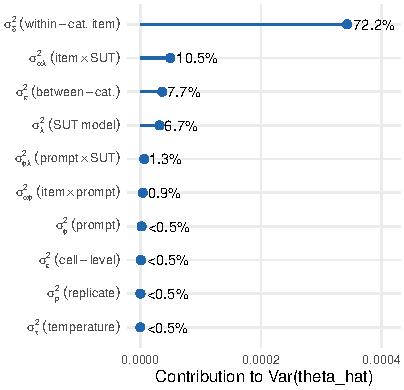
\includegraphics[width=\linewidth]{fig_mmlu_decomposition.pdf}\\
  \footnotesize (a) G-study: variance decomposition
\end{minipage}\hfill
\begin{minipage}[t]{0.49\linewidth}
  \centering
  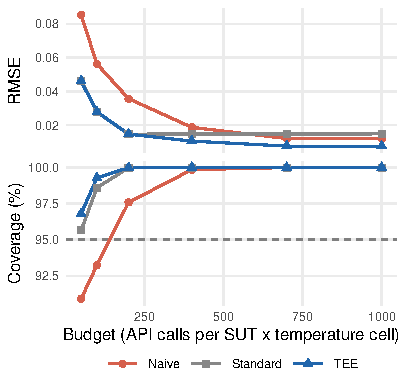
\includegraphics[width=\linewidth]{fig_budget_allocation_stacked.pdf}\\
  \footnotesize (b) D-study: budget allocation
\end{minipage}
\caption{MMLU G-study (a) and D-study (b). (a)~Contribution of each component to $\Var(\hat\theta)$ at the operational design ($N{=}200$, $V{=}4$, $M{=}3$ SUTs, $H{=}3$, $R{=}8$); item heterogeneity dominates, and the prompt terms together hold 2.7\%. (b)~RMSE against ground-truth accuracy (top) and 95\% CI coverage (bottom) by budget. TEE-guided allocation matches standard until the 170-item pool is used up, then keeps improving by averaging over prompt variants; naive, which replicates each call three times, has 1.6 to 2.4 times TEE's RMSE. 1,000 Monte Carlo replicates in each of the 9 SUT$\times$temperature cells at every budget level.}
\label{fig:mmlu_combined}
\end{figure}


\subsection{Chatbot Arena: Coverage, Accuracy, D-Study Validation}
\label{sec:arena}

Chatbot Arena \citep{chiang2024chatbot} extends our empirical tests to data comprising pairwise human votes that serve as ground-truth labels. LLM judges can stand in for human voters only if their scores hold up to the same standards as a human-rater study, with accuracy that does not depend on idiosyncratic prompt or judge choices. We test a TEE-guided pipeline against a naive single-judge baseline on 4,676 Arena matches drawn from the public release \texttt{lmarena-ai/arena-human-preference-100k}, stratified by (model $\times$ category) across Creative Writing, Coding, Factual QA, and Persuasion. Each match was scored under five chain-of-thought prompt variants by three judges, in both Likert (1 - 5 per response) and pairwise (A / B / tie, matching Chatbot Arena's voting UI) modes; full design details in SI Appendix, Section~\ref{si:arena}.

A Monte Carlo experiment that treats the full 4,676-match Likert factorial as a population ($p^* = 0.389$), shows that TEE averaging gives well-calibrated uncertainty. Naive 95\% Wald CIs computed from a single (judge, variant) cell hold nominal coverage at $n_m = 100$ matches but drop to 78\% coverage at $n_m = 2,000$ (Figure~\ref{fig:arena_coverage}). The TEE crossed random-effects Wald CI sits at or above 95\% throughout. The naive SE shrinks at $1/\sqrt{n_m}$ while between-cell variance does not, so at large $n_m$ the naive interval becomes a tight band around a single cell's mean. As in Figure 1, adding cases widens the coverage gap.

\begin{figure}[H]
\centering
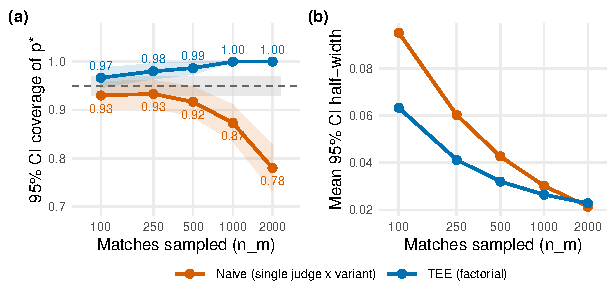
\includegraphics[width=0.75\linewidth]{fig_arena_coverage.pdf}
\caption{Naive coverage on Chatbot Arena drops as the sample grows, while TEE maintains nominal coverage. (a)~Empirical 95\% CI coverage versus match sample size $n_m$ for the naive single-judge, single-variant design and the TEE factorial design; ribbons show $\pm 1.96$ Monte Carlo SE over 300 replicates. (b)~Mean 95\% CI half-width versus $n_m$. The naive half-width shrinks as $1/\sqrt{n_m}$ while TEE bottoms out at the floor $\sigma_V^2/V + \sigma_J^2/J$ set by variant and judge variance. The target $p^* = 0.389$ is the mean over the 15 observed judge$\times$variant cells (3 judges, 5 variants), a finite-panel quantity. The TEE interval targets the superpopulation of prompts and judges from which those cells were drawn, so it carries between-cell variance the finite-panel target does not, and it over-covers that target at large $n_m$. An interval for the finite-panel target would hold the 5 variants and 3 judges fixed and bootstrap over matches only.}
\label{fig:arena_coverage}
\end{figure}

TEE averaging also improves per-match agreement with the individual human vote across all four categories (SI Appendix, Figure~\ref{fig:arena_accuracy}). Pooled across 4,676 matches, TEE Likert raises AB-only agreement over single-judge Likert by $+7.9$ pp (74.9\% vs.\ 67.0\%) and TEE pairwise raises it over single-judge pairwise by $+3.6$ pp (71.9\% vs.\ 68.3\%, see SI Appendix Table~\ref{tab:arena_agreement}). %Per-category lifts are positive in every cell, ranging from $+5.1$ to $+11.8$ pp for Likert and $+1.6$ to $+5.2$ pp for pairwise. %The Likert lift exceeds the pairwise lift in every category; pairwise judges almost never tie regardless of prompt wording, so the Likert-vs-pairwise comparison here is not a clean scoring-method contrast (SI Appendix, Section~\ref{si:arena}).

A D-study fit on 80\% of matches projects per-category SE reductions of 0.53 - 0.59 from single-judge to TEE. Across the four held-out categories, projected SE reductions track observed Likert agreement lifts at Spearman $\rho = 0.80$ (n = 4; SI Appendix Figure~\ref{fig:arena_dstudy_vs_observed}). Both gains matter when matches are scored one at a time, as in training on Arena labels \citep{egami2024dsl}.



\subsection{Single-Configuration Benchmarks Vulnerable to Benchmark Hacking}
\label{sec:gaming}

\citet{singh2025leaderboard} document Meta running 27 private Llama-4 variants on Chatbot Arena before launch and publishing only the top scorer (\emph{benchmark hacking}), which constitutes best-of-$K$ exploitation of pipeline noise. This can play out in a few ways: on hosted leaderboards, developers can submit many model variants under different identifiers and report only the best-scoring submission. On open-source benchmarks, they can rerun the evaluation internally with different prompt formats or scoring configurations until the score is favorable. The expected inflation is $\E[\max(Z_1,\ldots,Z_K)] \cdot \sigma_{\text{pipeline}}$, where $\sigma_{\text{pipeline}}$ is the standard deviation of the pipeline noise decomposed above. Prompt formatting alone can produce up to 76 accuracy points of spread on identical models \citep{sclar2024sensitivity}, suggesting the gameable surface is broad in practice.

We quantify the gaming surface in the context of Chatbot Arena by bootstrapping 4,676 matches across pipeline configurations (Figure~\ref{fig:gaming_surface}). The Arena human leaderboard already exposes a 45-Elo surface at $K{=}27$ from voter sampling alone, large enough to flip rankings between adjacent models. A single-configuration LLM-judge replacement ($V{=}1$, $M{=}1$) increases the surface to 56 Elo, since a developer can target both the LLM-judge configuration and the underlying voter sample. Averaging across either prompts or judges alone recovers the human baseline ($V{=}5$, $M{=}1$: 46 Elo; $V{=}1$, $M{=}3$: 46 Elo). TEE-LLM ($V{=}5$, $M{=}3$ averaging) cuts the surface to 32 Elo, about 30\% below the human leaderboard. Judge main effects account for the largest share of gameable LLM variance (Table~\ref{tab:gaming}), the component a developer most directly controls when picking judge models. Best-of-$K$ is one facet of the manipulation surface; \citet{singh2025leaderboard} also document score retraction, disproportionate sampling of proprietary models (61.4\% of battles), and Arena-specific data access that lifted Arena performance by up to 112\% without external gains.

\begin{figure}[htbp]
\centering
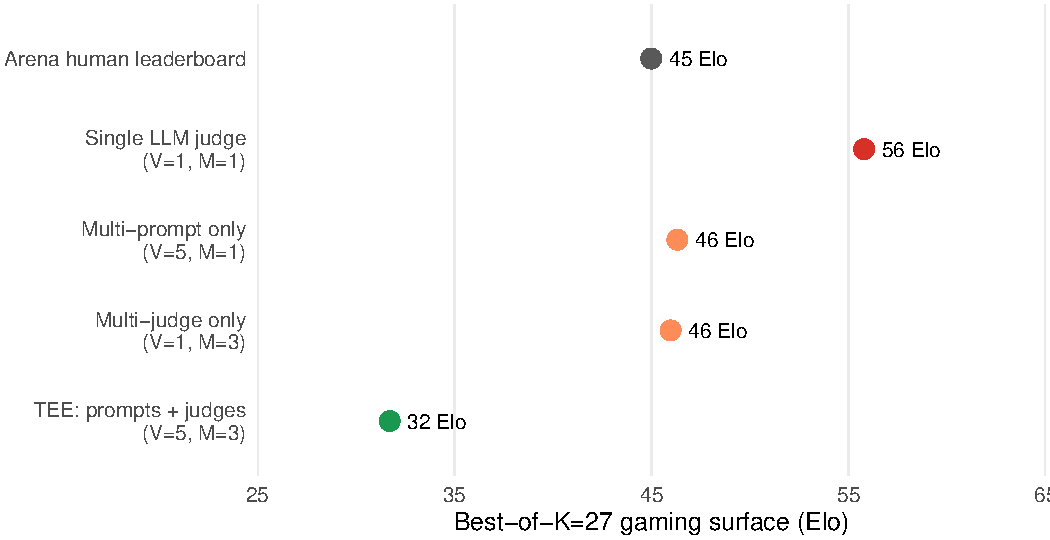
\includegraphics[width=0.8\linewidth]{fig_gaming_surface.pdf}
\caption{Best-of-$K{=}27$ gaming surface on Chatbot Arena across pipeline configurations. ``Gaming surface'' is the expected Elo boost a developer earns by submitting $K{=}27$ model variants and reporting only the highest-scoring one. Variance surface computed by bootstrapping 4,676 Arena matches.}
\label{fig:gaming_surface}
\end{figure}



\section{Discussion}
\label{sec:discussion}

Across the demonstrations, naive error estimates understate measurement uncertainty because they omit judge disagreement, prompt sensitivity, replicate noise, and their interactions. Evaluators then mistake pipeline noise for capability differences, and researchers mistake it for generalizable patterns in LLM-annotated data. The gap scales with the subjectivity and complexity of the task, and the Arena, MMLU, and propaganda results show that failing to average over these sources also costs accuracy. %: 43.8\% of $\Var(\hat\theta)$ in safety classification, 54.4\% in Likert ideology, and 68.4\% in pairwise ideology (with an additional 20.9\% for the position factor in pairwise). MMLU removes the judge layer, and item heterogeneity (35.0\%) and SUT-model design sensitivity (25.0\%) take over. 
%Deployment decisions, safety certifications, and published findings inherit the resulting error.

 %On MMLU, where each item is exact-match verified against an answer key (no rater), naive SE underestimates the TEE-corrected SE by 57\%. On the safety benchmark, where each item is a binary safe/unsafe call against a published taxonomy and most tasks are `safe,' the underestimate is 43\%. On Likert ideology, where raters compress a multi-dimensional judgment into a 1 - 5 score, the underestimate is 60\%. Full per-domain numbers in SI Appendix, Section~\ref{si:naive_vs_tee}.
 %The gaming analysis (Section~\ref{sec:gaming}) shows further that unmeasured pipeline variance means even routine model selection inflates reported scores.

Pipeline variance can also serve as a gaming surface in benchmarking and in research. We show that submitting best-of $K{=}27$ variants (as documented in \citet{singh2025leaderboard}) inflates Chatbot Arena Elo scores by 56 points, while averaging over multiple judges and prompts cuts that surface by 43\% (\S\ref{sec:gaming}). The same vulnerability extends to LLM-annotated research, where pipeline variance maps onto labeling error and predicts misclassification against the 9-rater human consensus in our propaganda demonstration ($r = -0.68$, SI Appendix, Section~\ref{sec:propaganda}), consistent with the configuration- and adversarial-search reversals \citet{baumann2025llmhacking} document across 37 LLM-annotation tasks. The implications extend beyond model capability overestimates, as benchmarks like SWE-Bench, LegalBench, and HealthBench inform estimates of labor substitution and productivity gains \citep{eloundou2023gpts} associated with widespread LLM adoption. 


%However beyond diagnosis, accounting for the total evaluation error (TEE) tells developers how to improve estimation. A small pilot run under our TEE framework yields variance estimates (e.g., confidence intervals) that naive estimates obscure, and a ranked list of which design changes would shrink it most (SI Appendix, Section~\ref{si:pilot}).

%Chatbot Arena's human votes let us test TEE end-to-end (\S\ref{sec:arena}). Across 4,676 matches, naive coverage falls as $N$ grows while TEE-corrected coverage holds; TEE averaging lifts agreement with human votes by 7.9 points; and D-study projections fit on 80\% of matches generalize to the held-out 20\%, validating the framework against ground-truth human data.

What transfers across pipelines? The structural lessons do. Claims are almost always about an item population, so more items beat fewer, and no score should hinge on a single judge or a single phrasing. The empirical rankings travel as priors. Wherever a judge layer is present, averaging over judges yields the largest single reduction in our projections, with items next on AILuminate and prompts next on Arena. The budget-relevant magnitudes are local estimates, and a pilot in the target pipeline should replace them before anyone spends on their basis.

Pipeline calibration is upstream of all real world benchmark use. When that output drives safety certification, LLM-annotated research, and labor-market projections, underestimated uncertainty propagates into each downstream decision. Our TEE framework allows for calibrated CIs at a fraction of that downstream cost.

% In naive estimation, the variance from prompts, judges, and their interactions is not averaged in pipeline variance estimates and omitted from CIs. The omission causes the under-coverage; the unaveraged variance is what a developer running best-of-$K$ exploits. The TEE-reducible share of $\sigma^2_{\text{pipeline}}$ therefore quantifies both with one number. Multi-judge multi-prompt averaging fixes both, cutting the Arena gaming surface by 43\% to below the human-leaderboard baseline.

% The rankings tend to converge on a common prescription across the demonstrations. Where a judge layer is present, averaging over judges produces the largest single variance reduction available, 37 - 45\% on AILuminate and Arena%, because $\sigma^2_\lambda/M$ and $\sigma^2_{\alpha\lambda}/(NM)$ both shrink with $M$
% . After judges, items matter most on AILuminate, prompts on Arena, and the two are comparable on MMLU (which has no judge). %Once those moves are made, additional replications buy little extra precision: they reduce $\sigma^2_\rho/(N'V'H'M'R')$, already a tiny fraction of $\Var(\hat\theta)$, but not the cell-level term $\sigma^2_\epsilon/(N'V'H'M')$, which lacks $R'$ in its denominator.

\section{Limitations}
\label{sec:limitations}


TEE has a number of simplifying assumptions worth noting. When a model emits reasoning traces, the variance they generate is not attributed under the current framework and instead inflates $\sigma^2_\epsilon$. When the scoring function relies on an LLM-as-judge, its variance may compound with the SUT's \citep{haldar2025roulette, chehbouni2025neither}, and any SUT$\times$judge interactions this introduces fall outside the within-layer decomposition (SI Appendix, Section~\ref{si:coverage}). Variance shares are reported on the probability scale and therefore assume an LPM, which generally preserves qualitative rankings but not precise magnitudes compared with a logistic link function (SI Appendix, Section~\ref{si:glmm}).

Perhaps more importantly, TEE cannot say whether the items span the construct of interest, which of course limits generalizability. Total survey error has long called this coverage error \citep{sen2019tedon}, and a toxicity benchmark that omits coded hate speech will yield precise but domain-incomplete estimates. 

Finally, all demonstrations are in English and use frontier models, leaving high-ambiguity tasks (creative writing, open-ended reasoning) untested. The full factorial design requires $\sim$54,000 API calls, though a pilot subset can deploy much of the framework in practice.


\section{Conclusion}
\label{sec:conclusion}

Confidence intervals in LLM evaluation are systematically too narrow, and benchmarks reward optimization against measurement noise. Beyond diagnosis, TEE lets analysts run D-study projections from a small pilot to recover honest CIs and rank which design changes would most reduce noise (SI Appendix, Section~\ref{si:pilot}). As evaluations increasingly shape deployment decisions, safety certifications, regulatory standards, and projections of AI's labor-market and economic impact, closing this gap is necessary before evaluation scores can support the high-stakes judgments they inform.

\begin{ack}
Thanks to Chris Barrie, Ben Guinaudeau, Aaron Kaufman, Brandon Stewart, Kylan Rutherford, and participants at the 2026 CSMAP conference for helpful feedback. Thanks to Peter Mattson, Bennett Hillenbrand, Andrew Gruen, Rebecca Weiss, Hannah Waight, Molly Roberts, Brandon Stewart, Eddie Yang, Ben Guinaudeau, Melina Much, Chris Barrie, Joe Higton, Kylan Rutherford, Jennifer Allen, Jonathan Nagler, and Josh Tucker for helpful early conversations about the problem of confidence intervals in LLM evals, benchmarks, and LLM-as-judge measurement problems, which helped inspire this paper.

MLCommons funded the author's salary for this work.

The author has personal financial interests in AI-related companies, in particular Nvidia, Alphabet, Microsoft, and Taiwan Semiconductor. The author worked at Facebook (now Meta) in various capacities from 2011 to 2015 and 2018 to 2020 and at Twitter (now X) from 2021 to 2023, and contracts for MLCommons, a 501(c)(6) non-profit that releases AI benchmarks, including AILuminate, which this paper analyzes (2026 to present). The author has accepted a position at Google DeepMind. For an unrelated project, the author received a 2010 Google Research Award for research on ``Social cues and reliability in content selection and evaluation.''
\end{ack}

\bibliographystyle{plainnat}
\bibliography{references}

% ----------------------------------------------------------------------
% Appendix — does not count against the 9-page limit. Phase 2 will paste
% content from paper/pnas_si_body.tex here, preserving si:* labels.
% ----------------------------------------------------------------------
\appendix
% NeurIPS appendix - migrated verbatim from paper/pnas_si_body.tex
% Section/table/figure/equation numbering is reset by \appendix in neurips_main.tex.
% All si:* labels preserved for cross-references from main text.


\section{Quickstart Guide}
\label{si:quickstart}

This guide walks through the operational pipeline for diagnosing uncertainty in an LLM annotation workflow. The full framework and derivations appear in Section~\ref{si:framework}.

\begin{enumerate}\setlength{\itemsep}{6pt}
\item \textbf{Run a small pilot.} A small pilot at a fixed temperature can estimate the dominant variance components when the judge layer is varied. The minimum design uses 30 or more items, 3 or more prompt variants, 2 or more judges (when a judge layer exists), and 3 or more replications, for roughly 540 API calls if evaluating a single scoring function. Variants share task instruction, output format, and reasoning mode but may differ in word choice, sentence structure, and framing of the construct (Section~\ref{si:framework}, Assumption~\ref{asn:exchangeability}). This broad operationalization reflects the prompt-wording uncertainty a real evaluator faces. Both strict paraphrases (e.g., prompting Claude Haiku at temperature 0.9 to rewrite a seed instruction $V$ ways) and small sets of templates that vary the framing of the construct are valid. The latter produces a broader $\hat{\sigma}^2_\phi$. Include the original benchmark prompt as one of the $V$ variants where one exists. Items should be drawn from the target deployment domain. Drop the judge facet for benchmarks without one (e.g., MMLU).

\item \textbf{Fit the variance decomposition.} The \texttt{totalevalerror} R package (\codeurl) wraps the variance decomposition, D-study, and budget-allocation routines from this paper:
\begin{verbatim}
library(totalevalerror)
des <- tee_design(pilot_df,
        outcome = score, item = item_id,
        prompt = variant_id, judge = judge_model,
        temperature = temp, replicate = rep,
        scoring = "binary")
fit <- tee_decompose(des)
\end{verbatim}
The fit reports each variance source as a share of $\Var(\hat\theta)$, and the largest share identifies the bottleneck. If judge variance ($\sigma^2_\lambda$) or item$\times$judge ($\sigma^2_{\alpha\lambda}$) dominates, as in the safety demonstration, adding judges helps most; if within-cell replicate noise ($\sigma^2_\rho$) leads, more replications buy precision; if prompt sensitivity ($\sigma^2_\phi$) dominates, more prompt variants help; if item heterogeneity ($\sigma^2_\alpha$) leads, more items help. The underlying fixed-temperature \texttt{lmer} formula is \texttt{score \textasciitilde{} judge + (1|item) + (1|prompt\_variant) + (1|item:prompt\_variant) + (1|item:judge) + (1|prompt\_variant:judge) + (1|item:prompt\_variant:judge)}, with the judge terms dropped for benchmarks without a judge layer. The final random effect captures cell-level idiosyncrasy; the \texttt{lmer} residual captures within-cell replicate noise. Users who prefer to fit it directly can do so.

\item \textbf{Optimize with the D-study.} \texttt{tee\_dstudy(fit)} returns projected SEs across alternative production designs (varying replications, prompt variants, judges, scoring methods). \texttt{tee\_budget\_allocate(fit, budget = X)} returns the cost-minimizing allocation under a fixed API budget. The projection is qualitatively reliable at pilot scale (Section~\ref{si:pilot}). The rank ordering of interventions transfers to the full design even when component magnitudes shift.

\item \textbf{Deploy and estimate CIs.} Apply the chosen production design to the full corpus, then call \texttt{tee\_se(fit)} for the corrected SE and \texttt{tee\_theta\_ci(fit, level = 0.95)} for a 95\% CI on $\hat\theta$. Because the formula incorporates the components naive CIs leave out (prompt and judge variance, plus their interactions), coverage holds near nominal even as sample size grows.

\item \textbf{Report.} \texttt{tee\_writeup(fit)} produces a paragraph summarizing the decomposition, the dominant variance components, the corrected CI, and the D-study-recommended design. For each scored measurement, also report the exact prompt text, model version, temperature, and number of replications. A tiered reporting checklist appears in Section~\ref{si:checklist}, Table~\ref{tab:checklist}.
\end{enumerate}


\clearpage

\section{Uncertainty Reporting in Current LLM Evaluation Practice}
\label{si:current_practice}

Table~\ref{tab:current_practice} surveys uncertainty reporting across thirteen widely used LLM benchmarks and annotation studies. Two patterns stand out. In our 13-benchmark survey, most benchmarks report no measurement uncertainty at all. MMLU, the Open LLM Leaderboard, MT-Bench, SWE-bench, and ARC-AGI all provide only a point estimate. The four that do report CIs (AlpacaEval, HELM, Chatbot Arena, Arena-Hard) capture only item-sampling variance, leaving prompt sensitivity, judge variance, temperature, and interactions unmeasured. Contamination is also widespread. All six benchmarks with public test sets (MMLU, AlpacaEval, HELM, MT-Bench, Arena-Hard, SWE-bench) have documented training-data leakage, and even Chatbot Arena leaks historical votes back into training data despite its live-query design. AILuminate's private Official set and ARC-AGI's held-out tasks are the only contamination-resistant designs in the survey.

The bottom row shows TEE addressing every TEE-decomposition column simultaneously: prompt sensitivity, judge model and temperature, replications, interactions, item sampling, and the basic CI/SE indicator. The remainder of this section walks through each benchmark in detail.

% \begin{table}[htbp]
% \centering
% \small
% \caption{Most major benchmarks account only for single-item variance, if at all.}
% \label{tab:main_practice}
% \begin{tabular}{@{}lccccc@{}}
% \toprule
%  & Item & Prompt & Temp. & Judge & Inter. \\
% \midrule
% MMLU        & -        & - & - & n/a & - \\
% SWE-bench   & -        & - & - & n/a & - \\
% ARC-AGI     & -        & - & - & n/a & - \\
% AILuminate  & $\star$ & - & - & $^{\star}$ & - \\
% AlpacaEval     & $\star$ & - & - & - & - \\
% Chatbot Arena  & $\star$ & - & - & n/a & - \\
% \midrule
% TEE & $\star$ & $\star$ & $\star$ & $\star$ & $\star$ \\
% \bottomrule
% \end{tabular}
% \end{table}


\begin{table}[ht]
\centering
\small
\caption{Uncertainty reporting in prominent LLM evaluations. SUT-layer columns capture variance in the system under test. Judge-layer columns capture variance in the scoring pipeline.}
\label{tab:current_practice}
\resizebox{\textwidth}{!}{%
\begin{tabular}{@{}lcc ccc ccc cl@{}}
\toprule
 & & & \multicolumn{3}{c}{\textit{SUT layer}} & \multicolumn{3}{c}{\textit{Judge layer}} & & \\
\cmidrule(lr){4-6} \cmidrule(lr){7-9}
 & \rotatebox{70}{Any CI/SE} & \rotatebox{70}{Item sampling} & \rotatebox{70}{SUT prompt} & \rotatebox{70}{SUT temperature} & \rotatebox{70}{SUT replications} & \rotatebox{70}{Judge prompt} & \rotatebox{70}{Judge model} & \rotatebox{70}{Judge temperature} & \rotatebox{70}{Interactions} & \rotatebox{70}{Contamination} \\
\midrule
MMLU \citep{hendrycks2021mmlu} & - & - & - & - & - & n/a & n/a & n/a & - & High \\
Open LLM Leaderboard & - & - & - & - & - & n/a & n/a & n/a & - & Mixed \\
AlpacaEval \citep{dubois2024alpacaeval} & $\star$ & $\star$ & - & - & - & - & - & - & - & High \\
HELM \citep{liang2023helm} & $\star$ & $\star$ & - & - & - & n/a & n/a & n/a & - & High \\
Chatbot Arena \citep{chiang2024chatbot} & $\star$ & $\star$ & - & - & - & n/a & n/a & n/a & - & Medium \\
MT-Bench \citep{zheng2023llmjudge} & - & - & - & - & - & - & - & - & - & High \\
Arena-Hard \citep{li2024arenahard} & $\star$ & $\star$ & - & - & - & - & - & - & - & High \\
SWE-bench \citep{jimenez2024swebench} & - & - & - & - & - & n/a & n/a & n/a & - & High \\
ARC-AGI \citep{chollet2024arcagi} & - & - & - & - & - & n/a & n/a & n/a & - & Low \\
AILuminate \citep{ghosh2025ailuminate} & ($\star$) & - & - & - & - & - & ($\star$) & - & - & Medium \\
Gilardi et al.\ \citep{gilardi2023chatgpt} & - & - & n/a & n/a & n/a & - & - & - & - & n/a \\
T{\"o}rnberg \citep{tornberg2025llm} & - & - & n/a & n/a & n/a & - & - & - & - & n/a \\
Ziems et al.\ \citep{ziems2024css} & - & - & n/a & n/a & n/a & ($\star$) & ($\star$) & - & - & n/a \\
\midrule
\textbf{TEE} & $\star$ & $\star$ & $\star$ & $\star$ & $\star$ & $\star$ & $\star$ & $\star$ & $\star$ & n/a \\
\bottomrule
\multicolumn{11}{@{}l}{\footnotesize Deterministic scoring (exact match or test suite), no judge layer.} \\
\multicolumn{11}{@{}l}{\footnotesize Public test set with documented training-data leakage \citep{xu2024benbench}.} \\
\multicolumn{11}{@{}l}{\footnotesize Most subtests public. GPQA gated to reduce contamination.} \\
\multicolumn{11}{@{}l}{\footnotesize Human voters, not an LLM judge layer.} \\
\multicolumn{11}{@{}l}{\footnotesize Live queries, but historical votes published and prompts recur across months.} \\
\multicolumn{11}{@{}l}{\footnotesize Bootstrap CI over items, captures item sampling only.} \\
\multicolumn{11}{@{}l}{\footnotesize Public task set with documented solution leakage into training data.} \\
\multicolumn{11}{@{}l}{\footnotesize Private held-out evaluation set with human-calibrated difficulty.} \\
\multicolumn{11}{@{}l}{\footnotesize Paper specifies bounds from evaluator false-safe/false-unsafe rates. Ensemble of evaluators fixed. Public leaderboard displays grade only.} \\
\multicolumn{11}{@{}l}{\footnotesize Public DEMO subset (1,200 prompts) and public Practice set (12,000), with private Official test set (12,000).} \\
\end{tabular}%
}
\end{table}

\paragraph{MMLU and the Open LLM Leaderboard.} MMLU \citep{hendrycks2021mmlu} evaluates each model once on a fixed test set (14,079 items) with a single prompt format. For open-weight models with accessible logits, the standard implementation (EleutherAI lm-evaluation-harness) scores by comparing log-likelihoods of the full answer text for each of the four choices. For API-only models, the evaluation generates text and parses the answer letter, reintroducing temperature dependence and replicate noise. In both cases, no uncertainty is reported. The dominant missing uncertainty is item heterogeneity. On our 200-item factorial decomposition (SI Appendix, Section~\ref{si:mmlu}), within-category item heterogeneity contributes 72.2\% of $\Var(\hat\theta)$, item$\times$SUT 10.5\%, between-category heterogeneity 7.7\%, and SUT-model design sensitivity 6.7\% at the operational design. The three prompt terms together hold 2.7\%. \citet{sclar2024sensitivity} document up to 76 accuracy points of spread from formatting choices alone on MMLU. Those formatting perturbations are distinct from the phrasing-and-framing variants used in this paper (Assumption~\ref{asn:exchangeability}). Different implementations of MMLU (original, HELM, HuggingFace) also use different prompt templates and produce different rankings for the same models \citep{alzahrani2024benchmarks}. The Open LLM Leaderboard follows similar practice. Most of its subtests use public test sets, with GPQA gated to reduce contamination.

\paragraph{AlpacaEval.} AlpacaEval 2.0 \citep{dubois2024alpacaeval} uses a single LLM judge (GPT-4 Turbo) with a single prompt to score model outputs against a reference set. It reports a standard error capturing item-sampling variance. Every other pipeline factor is held to a single value (one judge, one prompt, one temperature, no replications), with none decomposed. A different judge model would produce a different win rate, but judge variance ($\sigma^2_\lambda$) is not measured. The length-controlled variant adjusts for response length but not for pipeline configuration variance.

\paragraph{HELM.} HELM \citep{liang2023helm} evaluates each model on each scenario with a fixed prompt format and runs 3 random seeds over different in-context example selections to increase stability. All prompts, predictions, and test items are publicly inspectable, which aids reproducibility but also makes HELM vulnerable to test-set contamination through training data leakage \citep{xu2024benbench}. Scoring uses deterministic automated metrics (accuracy, BLEU, ROUGE, F1), not LLM judges, so the judge layer does not apply. SUT prompt sensitivity (one format per scenario) and temperature effects (fixed) both apply but are not measured.

\paragraph{Chatbot Arena.} Chatbot Arena \citep{chiang2024chatbot} computes Bradley-Terry \citep{bradley1952rank} coefficients (labeled as Elo ratings) via maximum likelihood estimation with sandwich robust standard errors, collecting an average of roughly 8,000 votes per model. Prompt wording varies organically across users but is not controlled or decomposed. Voter heterogeneity (different humans rank differently) and SUT temperature (fixed per model by the provider) both apply but are not separated from sampling noise. The bootstrap CIs capture vote-sampling uncertainty but not the model-variant selection effects documented by \citet{singh2025leaderboard}, where providers tested dozens of private variants and published only the highest-scoring one.

\paragraph{MT-Bench.} MT-Bench \citep{zheng2023llmjudge} evaluates SUTs on 80 multi-turn questions (2 turns each, 8 categories) scored 1 - 10 by GPT-4. The judge model version is not pinned in the codebase, creating a reproducibility concern as the alias resolves to different model snapshots over time. The evaluation runs one prompt template per item at judge temperature 0 with no replications and no CI. SUT temperature varies by category (0.0 - 0.7). The LMSYS team's own later analysis found that only 22.6\% of model pairs have non-overlapping CIs on MT-Bench, compared with 87.4\% on Arena-Hard \citep{li2024arenahard}, so MT-Bench scores cannot statistically distinguish most model pairs.

\paragraph{Arena-Hard.} Arena-Hard-Auto \citep{li2024arenahard} evaluates SUTs on 500 challenging user queries drawn from Chatbot Arena, scored by GPT-4-Turbo in pairwise comparison against a baseline (GPT-4-0314). A two-game position-swap design mitigates position bias. Bootstrap CIs (100 resamples) capture item-sampling variance but not judge variance (single judge, single prompt template, single temperature = 0, no replications). Arena-Hard achieves 87.4\% model-pair separability, the highest among automated benchmarks tested. The test set is public.

\paragraph{SWE-bench.} The SWE-bench family \citep{jimenez2024swebench} evaluates coding agents on real GitHub issues. SWE-bench Verified (500 human-validated Python tasks) was the standard until contamination was documented across all frontier models. SWE-bench Pro (1,865 tasks drawn from 41 repositories, requiring $\geq$10 lines and averaging 4.1 files per fix) was introduced as a harder, less contaminated alternative. Scoring is deterministic. The agent's patch is applied and the repository test suite is run. Pass@1 (single attempt) is the standard metric. No CI is reported. The judge layer does not apply (test suites are deterministic). SUT prompt format, temperature, and replications all affect the generated patch but are not varied or decomposed.

\paragraph{ARC-AGI.} The ARC-AGI benchmark \citep{chollet2024arcagi} evaluates abstract reasoning on grid-transformation tasks, with versions of increasing difficulty: ARC-AGI-1 (2019, now largely solved with frontier models exceeding 96\%), ARC-AGI-2 (2025, frontier models reach $\sim$77\%), and ARC-AGI-3 (2026, interactive reasoning). For the static versions (1 and 2), scoring is exact match with up to two guesses per input. Version 3 uses an action-based protocol. Private held-out evaluation sets (100 - 120 tasks per version) and human-calibrated difficulty (400+ participant live studies for version 2) reduce contamination risk. No CI is reported. The score is a point estimate with no uncertainty quantification, though ARC-AGI-2 introduced a cost-per-task efficiency metric.

\paragraph{AILuminate.} AILuminate v1.0 \citep{ghosh2025ailuminate} evaluates SUT safety across 12 hazard categories (1,000 prompts each in the public Practice set and 12,000 in the private Official set, plus a 1,200-prompt Creative Commons DEMO subset). Scoring uses a fixed ensemble of safety evaluator models that flag violations, and final grades (Poor/Fair/Good/Very Good/Excellent) reflect the SUT's violation rate relative to a reference model. The technical paper specifies a methodology for computing upper and lower score bounds from evaluator false-safe and false-unsafe rates (uniquely among the benchmarks surveyed here), but the public leaderboard displays only the categorical grade. The methodology does not decompose item sampling, prompt sensitivity, evaluator-model choice (ensemble is fixed), or their interactions, and the paper acknowledges ``considerable variance in test outcomes'' from prompt sampling and evaluator noise without quantifying these sources separately.

\paragraph{LLM-as-annotator studies.} \citet{gilardi2023chatgpt} compare ChatGPT (GPT-3.5-turbo) annotations to trained research-assistant labels on political text classification, reporting accuracy and intercoder agreement (Cohen's $\kappa$, \citealt{cohen1960kappa}). The study does vary temperature (1.0 and 0.2) and collects two responses per setting, finding 91\% intercoder agreement between two ChatGPT runs at $T = 1$ and 97\% at $T = 0.2$. Gilardi et al.\ is a methods validation paper, not a downstream analysis, so the absence of pipeline-variance CIs is not itself a problem. Subsequent annotation studies follow the same single-configuration practice: \citet{tornberg2025llm} use GPT-4 with a single zero-shot prompt on political tweets. \citet{heseltine2024llm} compare GPT-4 expert coding across four countries with a single prompt and temperature. \citet{ziems2024css} survey 25 computational social science benchmarks and find the pattern pervasive. \citet{carlson2026smj} provide guidelines for management research, warning that small implementation choices can significantly affect LLM annotations and alter downstream findings. The single-configuration practice has been widely adopted for downstream hypothesis testing, where LLM annotations serve as variables in regressions and the pipeline variance TEE quantifies directly affects statistical conclusions \citep{baumann2025llmhacking, egami2024dsl}.



\clearpage

\section{Full Framework: Assumptions, Derivations, and Extensions}
\label{si:framework}

The sections below present the formal assumptions, variance decomposition, two-tier classification, heteroscedastic extension, and estimation details summarized in the main text.

\subsection{Model Terms and Factor Classification}

Table~\ref{tab:factors} classifies the factors in the TEE data-generating process.

\begin{table}[ht]
\centering
\caption{Factors in the TEE data-generating process (DGP), classified as fixed or random. Random factors (item, prompt variant, replication) represent exchangeable draws from larger populations. Their variance components shrink with aggregation \emph{within a chosen design} (Tier~1). Fixed factors (temperature, model, scoring method) represent specific researcher choices. When no aggregation occurs, their sensitivity indices quantify researcher degrees of freedom (Tier~2). When the design \emph{does} cross multiple levels of a fixed factor (e.g., averaging over a panel of judges), the corresponding sensitivity contribution also shrinks as $1/L$. This across-design aggregation is what the empirical sections rely on for judge-model averaging.}
\label{tab:factors}
\small
\begin{tabular}{lllp{5.5cm}}
\toprule
\textbf{Factor} & \textbf{Type} & \textbf{Levels} & \textbf{Examples} \\
\midrule
Item $i$ & Random & $N$ (large) & A specific social media post; a safety test prompt together with the SUT response being judged \\
Category $c$ & Random grouping & $C$ & Hate speech type, hazard category \\
Prompt variant $v$ & Random & $V$ (3 - 5) & ``Is this post hateful?'' vs.\ ``Does this contain hate speech?'' \\
Temperature $h$ & Fixed & $H$ (e.g., 3) & $T = 0.0, 0.7, 1.0$ \\
Model $m$ & Fixed & Small set & GPT-4o, Claude Haiku~4.5, Gemini~2.0 Flash \\
Scoring method & Fixed (Tier 2) & Typically 1 & Exact match, Likert, LLM-as-judge \\
Replication $r$ & Random (nested) & $R$ (5 - 10) & Repeated API call with identical inputs \\
\bottomrule
\end{tabular}
\end{table}

\begin{table}[ht]
\centering
\caption{Exploitable variance components in single-configuration benchmarks (Chatbot Arena Likert decomposition, pooled across the four categories). Empirical shares from the full-factorial decomposition (4,676 matches, 5 prompt variants, 3 judges). Reported as shares of per-observation variance $\sigma^2_\text{total}$ because gaming exploits single-configuration noise directly, before averaging shrinks any component. ``How it inflates scores'' describes two channels: (1)~passive inflation, where the benchmark operator's single-configuration design leaves noise that widens CIs for all submissions, and (2)~active exploitation, where a developer who can probe the benchmark's specific configuration optimizes against it.}
\label{tab:gaming}
\small
\begin{tabular}{p{2.8cm}p{1.8cm}p{4.5cm}p{4cm}}
\toprule
\textbf{Variance component} & \textbf{Empirical share} & \textbf{How it inflates scores} & \textbf{Mitigation} \\
\midrule
Prompt sensitivity $\sigma^2_\phi$ & 1.2\% & \textit{Passive:} benchmark's single prompt carries unquantified phrasing noise. \textit{Active:} developer tunes output to the known prompt style & Average $\geq$3 diverse prompt variants \\
Judge model $\sigma^2_\lambda$ (fixed) & 8.8\% & \textit{Passive:} a single judge's systematic bias shifts all scores. \textit{Active:} developer optimizes for the specific judge's preferences & Multi-judge average or report all judges \\
Item$\times$prompt $\sigma^2_{\alpha\phi}$ & 2.5\% & \textit{Passive:} item-specific phrasing noise inflates CIs. \textit{Active:} developer targets responses the chosen prompt phrasing scores leniently & Multi-prompt averaging \\
Item$\times$judge $\sigma^2_{\alpha\lambda}$ & 18.0\% & \textit{Passive:} a single judge's item-level idiosyncrasies inflate CIs. \textit{Active:} developer fine-tunes on items the chosen judge scores leniently & Multi-judge averaging eliminates this interaction \\
Prompt$\times$judge $\sigma^2_{\phi\lambda}$ & 0.7\% & Specific (judge, prompt) cell biases compound when both are fixed & Multi-prompt $\times$ multi-judge averaging \\
\bottomrule
\end{tabular}
\end{table}

The unit of analysis is a single ``item'' (a benchmark case, social media post, or similar) scored once at one combination of prompt variant, temperature, model, and replication. A typical pipeline involves two LLM calls, with the system under test (SUT) generating an output and a judge scoring it. The DGP applies to one layer at a time. At the judge layer, ``item'' is a (prompt, SUT-response) pair; at the SUT layer, ``model'' indexes SUTs and the variance components capture SUT-side properties. The default target estimand is $\theta_{hm} = \E_{i,v,r}[Y_{ivhm}^{(r)}] = \mu + \tau_h + \lambda_m$, the expected value of the scored output over exchangeable items, prompt variants, and replications, conditional on fixed design choices. TEE quantifies how much uncertainty surrounds $\hat{\theta}_{hm}$ from each step of the pipeline.

Whether each factor enters as fixed or random depends on whether exchangeability holds across its levels. Temperature is fixed because different temperature levels produce qualitatively different generation regimes that violate exchangeability (Section~\ref{si:temperature}). Prompt variants are random because phrasing-and-framing variants drawn from a larger space of equivalent reformulations plausibly satisfy exchangeability, provided no single variant is systematically better than the others and all variants share the same reasoning mode and output format (Assumption~\ref{asn:exchangeability}). Scoring method is treated as fixed because it shapes the residual distribution and interacts with prompt sensitivity, and it enters as an additional fixed factor when the design varies it.

When items belong to content categories, $\alpha_i = \kappa_{c(i)} + \delta_{i|c}$, where $\kappa_c \sim N(0, \sigma^2_\kappa)$ captures between-category variance and $\delta_{i|c} \sim N(0, \sigma^2_\delta)$ captures within-category heterogeneity:
\begin{equation}
\sigma^2_\alpha = \sigma^2_\kappa + \sigma^2_\delta
\end{equation}

\subsection{Target Estimand}
\label{si:estimand}

The target estimand is the expected value of the scored output conditional on the researcher's fixed design choices (temperature $h$, model $m$):
\begin{equation}
\label{eq:estimand}
\theta_{hm} = \E_{i, v, r}\!\left[Y_{ivhm}^{(r)}\right] = \mu + \tau_h + \lambda_m
\end{equation}
where the expectation averages over random factors (items, prompt phrasings, replications) while conditioning on temperature and model. $\theta_{hm}$ is the ``universe score'' in generalizability theory \citep{bayerl2007gtheory, brennan2001gtheory}. When averaging over $H$ selected temperature levels, $\theta_m = \frac{1}{H}\sum_h \theta_{hm} = \mu + \bar{\tau} + \lambda_m$ is a finite average over those chosen levels. Analogously, a multi-judge target is a finite average over the selected judge panel, with $\sigma^2_\lambda$ measuring sensitivity inside that panel rather than a superpopulation variance over all possible judges.

Some benchmark reports instead target the exact finite item set already in hand. For that finite-benchmark estimand, item main effects are conditioned on rather than sampled, and the $\sigma^2_\alpha/N'$ term drops from the D-study formula. The remaining prompt, judge, temperature, interaction, cell-level, and replicate terms still quantify how much the reported score depends on measurement-pipeline choices for that item set.

TEE applies in three settings. The most direct case is when the measurement is itself the construct of interest, as in LLM benchmarking and LLM-as-judge evaluation where the scored output defines the quantity being measured. TEE also applies when pipeline stability is the goal in itself, since a pipeline with high measurement variance may not produce useful results even when unbiased on average. The third case is downstream analysis using LLM annotations as surrogate labels. Here $\theta_{hm}$ is a proxy for an external ground truth $\theta^* = \E[Y^*]$, and the surrogate labeling error $\tilde{Y} - Y^*$ introduces bias and variance not captured by TEE alone. Section~\ref{si:dsl} develops the formal connection to the DSL framework \citep{egami2024dsl} and shows how each TEE component maps to a term in the surrogate labeling variance.

Item heterogeneity ($\sigma^2_\alpha$) is partly signal and partly noise. Items genuinely differ in their true labels, which is a feature of the construct being measured and not a deficiency of the measurement procedure. A D-study that recommends adding more items improves precision (shrinks $\Var(\hat\theta_{hm})$) but not validity (the distance between $\theta_{hm}$ and $\theta^*$). Separating the signal component of $\sigma^2_\alpha$ from the noise component requires an external anchor such as human labels, known-answer items, or a validation sample, and lies outside TEE's scope.

The error bars cannot extrapolate beyond the item population named by the estimand, and assume the sampling frame covers the domain of interest. Precise TEE error bars may still produce misleading estimates if the item set omits key hazard categories. Section~\ref{si:coverage} discusses this boundary.

\subsection{Assumptions}

The decomposition requires the following assumptions:

\begin{assumption}[Conditional Exchangeability]
\label{asn:exchangeability}
Replications $r = 1, \ldots, R$ are exchangeable given $(i, v, h, m)$. Infrastructure nondeterminism \citep{yuan2025numerical} that varies across repeated calls is absorbed into $\rho_{ivhm}^{(r)}$; stable cell-level idiosyncrasy from omitted higher-order interactions is absorbed into $\epsilon_{ivhm}$. Similarly, prompt variants $v = 1, \ldots, V$ are exchangeable given item $i$. In other words, $\sigma^2_\phi$ captures sensitivity to both phrasing and framing within a fixed task instruction, output format, and reasoning mode. Variants share the canonical task and rubric structure but may differ in word choice, sentence structure, and the specific framing of the underlying construct. 

In the empirical demonstrations, prompt variants were authored as a small set of templates that vary framing while preserving task and output format, with the original benchmark prompt included where one exists; the propaganda demonstration also used an LLM paraphrase pipeline (\texttt{anthropic/claude-haiku-4.5}, temperature 0.9) on a seed instruction \citep{mizrahi2024multiprompt, barrie2024pss}. The safety and MMLU variants passed a deterministic format check and a construct-equivalence screen computed independently of the scores; one MMLU variant failed the format check and is excluded (Section~\ref{si:mmlu_parsing}). The Arena and propaganda variants predate the screen and were not screened. Section~\ref{si:prompt_admissibility} reports the screen, its validation against off-construct decoys, and how $\hat\sigma^2_\phi + \hat\sigma^2_{\alpha\phi}$ moves as the variant universe widens from strict paraphrase to construct reframing (flat for safety; 2.1\% to 20.6\% of G-study variance for MMLU). The reported $\hat{\sigma}^2_\phi$ is therefore an upper bound on what a strict-paraphrase design would estimate and a lower bound relative to broader framing sets or designs that also cross output format or reasoning mode; simulation confirms that D-study projections hold under exchangeability violations of this kind (Section~\ref{si:dstudy_validation}, Scenario~3).
\end{assumption}

\begin{assumption}[Additivity with Two-Way Interactions]
\label{asn:additivity}
Effects are additive up to two-way interactions. Higher-order interactions are absorbed into the residual. Monte Carlo evidence (Section~\ref{si:additivity}) shows that D-study projections tolerate three-way interactions with magnitudes up to 100\% of the largest two-way component. The restriction is testable via likelihood ratio test.
The compact formulas also omit fixed-by-fixed interactions such as temperature$\times$model. When a design crosses multiple fixed factors and their interaction is substantively large, add the corresponding finite sensitivity term to the D-study formula.
\end{assumption}

\begin{assumption}[Distributional Assumptions]
\label{asn:normality}
All random effects are normally distributed with mean zero and mutually independent. The normality assumption can be relaxed for REML estimation \citep{jiang1996reml}. Mutual independence is the more substantive assumption, with two violations warranting scrutiny. First, the model assumes item difficulty is independent of prompt sensitivity ($\alpha_i \perp (\alpha\phi)_{iv}$), yet ambiguous items may be more prompt-sensitive. Second, the model assumes difficulty is independent of temperature sensitivity ($\alpha_i \perp (\alpha\tau)_{ih}$), yet items near a decision boundary should be where temperature matters most. Section~\ref{si:dstudy_validation}, Scenario~2 shows that even strong dependence produces $\leq$2\% D-study bias.
The D-study formulas use pooled interaction variances across fixed levels. If item$\times$judge, item$\times$temperature, residual, or replicate variance differs sharply by fixed level, use stratum-specific variance estimates or the heteroscedastic extension; the pooled formula is inappropriate in that case.

For binary outcomes, the linear model is a linear probability model (LPM), adequate when baseline rates are moderate (0.3 - 0.7). At extreme rates, a GLMM robustness check is recommended (Section~\ref{si:glmm}).
\end{assumption}

\subsection{Variance Decomposition Derivation}

The variance of a single observation at fixed $h$ and $m$ follows from mutual independence of random effects:
\begin{equation}
\Var(Y \mid h, m) = \sigma^2_\alpha + \sigma^2_\phi + \sigma^2_{\alpha\phi} + \sigma^2_{\alpha\tau} + \sigma^2_{\phi\tau} + \sigma^2_{\alpha\lambda} + \sigma^2_{\phi\lambda} + \sigma^2_\epsilon + \sigma^2_\rho
\end{equation}

Averaging over $H$ temperatures introduces a design-sensitivity term:
\begin{equation}
\sigma^2_\tau = \frac{1}{H}\sum_{h=1}^{H}(\tau_h - \bar{\tau})^2
\end{equation}
This is computed from fixed effects, not REML, and depends entirely on which temperature levels the researcher chose. Model choice is analogous, with $\sigma^2_\lambda = \frac{1}{M}\sum_m(\lambda_m - \bar{\lambda})^2$.

The variance components divide into random-effect components, which shrink with more data, and fixed-effect sensitivity indices, which measure dependence on researcher choices. This partition maps onto the researcher degrees of freedom problem \citep{simmons2011falsepositive}, since temperature, scoring method, model, and system prompt are arbitrary choices that could have been made differently. TEE quantifies the sensitivity of $\hat{\theta}$ to each choice, analogous to the multiverse analysis of \citet{steegen2016multiverse}. Further design choices that can vary across runs include scoring or extraction method ($\sigma^2_{\text{extract}}$), system prompt ($\sigma^2_{\text{sys}}$), infrastructure ($\sigma^2_{\text{infra}}$), and temporal drift ($\sigma^2_{\text{drift}}$). \citet{barrie2025replication} catalogs these. Each enters as an additional fixed factor when the design varies it.

\subsection{Per-Observation Variance Decomposition}
\label{si:per_observation}

Often, statistical work decomposes variance at the observation level rather than for some aggregate quantity of interest ($\Var(\hat{\theta})$), as we do in the main-text and here in the SI. The per-observation share $\hat\sigma^2_k / \sigma^2_{\text{total}}$ characterizes the data-generating process before any aggregation.

The per-observation share is the right summary for understanding the structure of single LLM calls. Table~\ref{tab:gaming} reports per-observation shares to display the per-call variance profile. Gaming surfaces themselves are design-specific and are computed by bootstrap in Section~\ref{sec:gaming}.

The Var($\hat\theta$) share is the right summary for the analyst, who reports a quantity of interest like the mean and wants to know what fraction of its standard error comes from each source. Each component $\hat\sigma^2_k$ enters $\Var(\hat\theta)$ divided by the count of factor levels averaged over (e.g., $\sigma^2_\alpha/N$, $\sigma^2_\lambda/M$, $\sigma^2_\rho/(NVHMR)$), so a component with a large per-observation share but a large divisor contributes negligibly to mean variance. In the safety demonstration, replicate noise $\sigma^2_\rho$ is 21\% of per-observation variance but $<$0.5\% of $\Var(\hat\theta)$ at $R = 8$ because the divisor $NVHMR = 50{,}760$ erases its contribution. Conversely, judge-model design sensitivity $\sigma^2_\lambda$ is 0.8\% of per-observation variance but 43.8\% of $\Var(\hat\theta)$ because its divisor $M = 3$ leaves it almost intact.

Both summaries are computed from the same REML fit. Per-observation shares characterize the DGP and should be cited when comparing decomposition structure across studies, link functions, or scoring methods. Var($\hat\theta$) shares describe the analyst's mean SE under a specified design and should be cited when prescribing budget allocation, judge averaging, or sample-size choices.

\subsection{Estimation, Identifiability, and Diagnostics}
\label{si:estimation}

\paragraph{Estimation.} TEE uses REML via \texttt{lme4::lmer} in R. The base \texttt{lmer} call (cross-model design):
\begin{verbatim}
lmer(Y ~ temperature + model +
     (1|item) + (1|prompt_variant) +
     (1|item:prompt_variant) +
     (1|item:temperature) +
     (1|prompt_variant:temperature) +
     (1|item:model) +
     (1|prompt_variant:model) +
     (1|item:prompt_variant:model:temperature),
     data = df)
\end{verbatim}
Under category nesting, add \texttt{(1|category)}. Variance components are extracted via \texttt{VarCorr()}. Fixed-effect sensitivity indices use population variance ($1/H$, not $1/(H{-}1)$).

\paragraph{Boundary estimates.} Variance components at exactly zero (singular fits) occur routinely when the true variance is small. Report boundary estimates transparently. Bayesian alternatives with half-$t$ priors \citep{gelman2006prior} avoid boundary issues.

\paragraph{Identifiability.} The model requires a factorial design with every item evaluated under every prompt variant, at every temperature, and by every model. The minimum design uses $N \geq 30$ items, $V \geq 3$ prompt variants, and $R \geq 5$ replications. Prompt sensitivity ($\sigma^2_\phi$) is the hardest to estimate precisely ($V = 2$ produces 4 - 5\% bias, while $V \geq 3$ reduces bias to $<$4\%).

\paragraph{Diagnostics.} (1)~QQ plots of BLUPs \citep[best linear unbiased predictions;][]{robinson1991blup} for normality. (2)~Residual-vs-fitted plots for heteroscedasticity. (3)~Three-way interaction test via likelihood ratio. (4)~BLUP magnitude vs.\ item difficulty for independence violations. (5)~Category-level interaction decomposition.

\subsection{Heteroscedastic Extension}
\label{si:heteroscedastic}

The base model assumes common $\sigma^2_\epsilon$ and $\sigma^2_\rho$ across temperatures. In practice, greedy decoding and sampled decoding can produce different cell-level and replicate-level variances. The heteroscedastic extension replaces the common terms with $\epsilon_{ivhm} \sim N(0, \sigma^2_{\epsilon,h})$ and $\rho_{ivhm}^{(r)} \sim N(0, \sigma^2_{\rho,h})$, estimable via per-stratum REML in \texttt{lme4::lmer} (near-zero bias, $<$0.3\%) or via \texttt{nlme::lme()} \citep{pinheirobates2000} with \texttt{weights = varIdent}.

\subsection{D-Study Formulas: Full Derivation}

For a single model at fixed temperature, the projected variance of $\hat{\theta}_{hm}$ is
\begin{equation}
\Var(\hat{\theta}_{hm}) = \frac{\sigma^2_\alpha}{N'} + \frac{\sigma^2_\phi}{V'} + \frac{\sigma^2_{\alpha\phi}}{N'V'} + \frac{\sigma^2_{\alpha\tau}}{N'} + \frac{\sigma^2_{\phi\tau}}{V'} + \frac{\sigma^2_{\epsilon,h}}{N'V'} + \frac{\sigma^2_{\rho,h}}{N'V'R'}.
\end{equation}
Under category nesting, $\sigma^2_\alpha \to \sigma^2_\delta$ plus a $\sigma^2_\kappa/C'$ term, where $C'$ is the number of categories in the projected design. Averaging over $H$ temperatures gives
\begin{equation}
\Var(\hat{\theta}_m) = \frac{\sigma^2_\alpha}{N'} + \frac{\sigma^2_\phi}{V'} + \frac{\sigma^2_\tau}{H} + \frac{\sigma^2_{\alpha\phi}}{N'V'} + \frac{\sigma^2_{\alpha\tau}}{N'H} + \frac{\sigma^2_{\phi\tau}}{V'H} + \frac{\bar{\sigma}^2_\epsilon}{N'V'H} + \frac{\bar{\sigma}^2_\rho}{N'V'HR'}.
\end{equation}
Projecting across $M$ models at fixed temperature adds the model-related interaction terms,
\begin{equation}
\Var(\hat{\theta}_h) = \frac{\sigma^2_\alpha}{N'} + \frac{\sigma^2_\phi}{V'} + \frac{\sigma^2_\lambda}{M} + \frac{\sigma^2_{\alpha\phi}}{N'V'} + \frac{\sigma^2_{\alpha\tau}}{N'} + \frac{\sigma^2_{\phi\tau}}{V'} + \frac{\sigma^2_{\alpha\lambda}}{N'M} + \frac{\sigma^2_{\phi\lambda}}{V'M} + \frac{\bar{\sigma}^2_\epsilon}{N'V'M} + \frac{\bar{\sigma}^2_\rho}{N'V'MR'}.
\end{equation}
All three formulas follow from the expected mean squares (EMS) of the mixed design \citep[ch.~9]{brennan2001gtheory}. The EMS table appears in Section~\ref{si:gtheory}.
When averaging jointly over temperature and model, add the finite main-effect terms $\sigma^2_\tau/H$ and $\sigma^2_\lambda/M$. If their fixed-factor interaction is non-negligible, add $\sigma^2_{\tau\lambda}/(HM)$.

The safety classification design from Section~\ref{sec:safety} shows how these formulas convert real variance estimates into a confidence interval and which design changes they flag as high-leverage. The factorial covers $N = 141$ items spanning $C = 12$ hazard categories, with $V = 5$ prompt variants, $H = 3$ temperatures, $M = 3$ judge models, and $R = 8$ replications per cell. Variance components estimated on this design reveal that judge-model design sensitivity dominates at 43.8\% of $\Var(\hat\theta)$, item$\times$judge interaction adds 16.7\%, and prompt$\times$judge another 12.4\%. The three judge-related components together account for roughly 73\% of the variance budget. Within-category item heterogeneity contributes 20.8\%, and the remaining components each fall below 5\%. Plugging these into the multi-model formula yields $\Var(\hat\theta) = 0.000354$, $\text{SE}(\hat\theta) = 0.019$, and a 95\% CI of $0.942 \pm 0.037$ for the overall safe rate. The same formula reveals which design changes would shrink that variance further. Adding 5 replications above the existing 8 improves $\Var(\hat\theta)$ by less than 0.1\% because $\sigma^2_\rho/(NVHMR)$ is already a tiny share of the variance budget once divided by all four other factors. Committing to a single judge model inflates $\Var(\hat\theta)$ by 106\% because $\sigma^2_\lambda$ loses its $1/M$ averaging benefit. The dominance pattern and the counterfactuals point the same way, so the D-study directs additional spend toward more judges and items.



\subsection{Comparison with Concurrent Frameworks}
\label{si:comparison}

Table~\ref{tab:comparison} compares TEE with concurrent variance decomposition and uncertainty quantification frameworks for LLM evaluation.

\begin{table}[ht]
\centering
\caption{Feature comparison of TEE with concurrent frameworks for LLM evaluation uncertainty. Stars indicate features present. Dashes indicate absent or not addressed. Cell entries verified against each paper's text and tables.}
\label{tab:comparison}
\small
\begin{tabular}{lcccccc}
\toprule
\textbf{Feature} & \textbf{TEE} & \textbf{Camuffo} & \textbf{Haase} & \textbf{Song} & \textbf{Wang} & \textbf{NIST} \\
 & & \textbf{(2026)} & \textbf{(2026)} & \textbf{(2025)} & \textbf{(2025)} & \textbf{(2026)} \\
\midrule
G-theory grounded & $\star$ & $\star$ & - & $\star$ & - & - \\
Interaction terms & $\star$ & - & - & $\star$ & - & - \\
D-study projections & $\star$ & - & - & $\star$ & - & - \\
Two-tier separation & $\star$ & - & - & - & - & - \\
Scoring method comparison & $\star$ & - & - & - & - & - \\
Multi-domain replication & $\star$ & - & - & - & - & - \\
Monte Carlo validation & $\star$ & - & - & - & - & - \\
Multi-model factorial & $\star$ & $\star$ & $\star$ & - & - & $\star$ \\
Pilot-to-full validation & $\star$ & - & - & - & - & - \\
Prompt sensitivity & $\star$ & $\star$ & $\star$ & - & - & - \\
Temperature as factor & $\star$ & - & - & - & - & - \\
\# variance components & 9+ & 5 & 3 & varies & 2 & 2 \\
Empirical demonstrations & 4 & 1 & 1 & 1 & 1 & - \\
\bottomrule
\end{tabular}
\end{table}

These frameworks differ primarily in their grounding (G-theory versus ad hoc decompositions) and the number of variance components they separate. Camuffo et al.\ \citep{camuffo2026variance} develop a G-theory-grounded protocol for LLM annotation in strategy research with five variance sources and a sampling-budget specification, the closest framework in the variance-decomposition literature we surveyed. TEE extends this with formal interaction-term estimation (item$\times$judge contributes 16.7\% of $\Var(\hat\theta)$ in safety and the per-observation share ranges 13 - 44\% across the demonstrations here), D-study sample-size projections, the two-tier fixed/random classification, scoring method comparison, and Monte Carlo validation of D-study stability under assumption violations. Song et al.\ \citep{song2025gtheory} apply full G-theory to writing assessment with a person $\times$ rater $\times$ task design (run separately for one holistic and three analytic scoring dimensions) and D-study projections, a more complete psychometric application than the LLM-evaluation papers surveyed.

Haase et al.\ \citep{haase2026withinmodel} decompose variance into three components (model choice, prompt, within-model) without interaction terms or D-study projections. Wang \citep{wang2024measuring} uses an all-pairs paired-model method to decompose total noise into prediction noise (within-question) and data noise (between-question), without separately modeling prompt, temperature, or judge as facets in the decomposition. The NIST AI 800-3 report \citep{keller2026nist} proposes GLMMs for benchmark evaluation, citing G-theory as a parallel framing but without operationalizing D-study sample-size projections. Miller \citep{miller2024errorbars} applies the law of total variance to partition between-question and within-question variation, a two-component decomposition that TEE subsumes.



\clearpage

\section{G-Theory Connection and EMS Tables}
\label{si:gtheory}

Section~\ref{sec:gtheory} states the correspondence in the main text. TEE is an application of generalizability theory \citep[G-theory;][]{cronbach1972dependability, brennan2001gtheory} to LLM evaluation. Table~\ref{tab:gtheory} provides the mapping.

\begin{table}[ht]
\centering
\caption{Mapping between classical generalizability theory (G-theory) and TEE terminology. TEE applies G-theory's variance decomposition and decision-study framework to LLM evaluation pipelines, treating items as the object of measurement and prompt variants, judges, and replications as measurement facets.}
\label{tab:gtheory}
\small
\begin{tabular}{ll}
\toprule
\textbf{G-Theory} & \textbf{TEE} \\
\midrule
Object of measurement & Item $i$ \\
Facet (rater) & Model/judge $m$ \\
Facet (occasion) & Prompt variant $v$ \\
Fixed facet & Temperature $h$ \\
Universe score $\mu_p$ & $\theta_{hm} = \mu + \tau_h + \lambda_m$ \\
G-study & Factorial data collection \\
D-study & Pipeline optimization \\
$\sigma^2_p$ (object variance) & $\sigma^2_\alpha$ (item heterogeneity) \\
$\sigma^2_r$ (rater variance) & $\sigma^2_\lambda$ (model sensitivity) \\
$\sigma^2_{pr}$ (object $\times$ rater) & $\sigma^2_{\alpha\lambda}$ (item $\times$ model) \\
\bottomrule
\end{tabular}
\end{table}

Table~\ref{tab:ems} gives the expected mean squares for the balanced mixed design.

\begin{table}[ht]
\centering
\caption{Expected mean squares for the balanced mixed design with $C$ categories, $n = N/C$ items per category, $V$ prompt variants, and $R$ replications, conditioning on model $m$ and temperature $h$. Temperature interaction terms ($\sigma^2_{\alpha\tau}$, $\sigma^2_{\phi\tau}$) are confounded with item and prompt main effects at a single temperature level. A multi-temperature design adds rows for Temperature ($H-1$ df), Item$\times$Temperature, and Prompt$\times$Temperature.}
\label{tab:ems}
\small
\begin{tabular}{lll}
\toprule
\textbf{Source} & \textbf{df} & \textbf{EMS} \\
\midrule
Category ($\kappa$) & $C - 1$ & $\sigma^2_\rho + R\sigma^2_\epsilon + R\sigma^2_{\alpha\phi} + VR(\sigma^2_\delta + \sigma^2_{\alpha\tau}) + nVR\sigma^2_\kappa$ \\
Item w/in cat.\ ($\delta$) & $C(n-1)$ & $\sigma^2_\rho + R\sigma^2_\epsilon + R\sigma^2_{\alpha\phi} + VR(\sigma^2_\delta + \sigma^2_{\alpha\tau})$ \\
Prompt ($\phi$) & $V - 1$ & $\sigma^2_\rho + R\sigma^2_\epsilon + R\sigma^2_{\alpha\phi} + NR(\sigma^2_\phi + \sigma^2_{\phi\tau})$ \\
Item $\times$ Prompt ($\alpha\phi$) & $(N-1)(V-1)$ & $\sigma^2_\rho + R\sigma^2_\epsilon + R\sigma^2_{\alpha\phi}$ \\
Residual ($\rho$) & $NV(R-1)$ & $\sigma^2_\rho$ \\
\bottomrule
\end{tabular}
\end{table}

Solving the EMS equations for the variance of the grand mean $\bar{Y}_{\cdot\cdot h}$ yields the D-study formulas above. Model-related interactions ($\sigma^2_{\alpha\lambda}$, $\sigma^2_{\phi\lambda}$) enter under the multi-model extension (D-study Case~3 above) and are not shown in this single-model EMS table.



\paragraph{Absolute versus relative error.} The D-study formulas above give the \emph{absolute} error variance, appropriate for threshold decisions (``does this model exceed 80\% safety?''). For \emph{relative} decisions (comparing two models or ranking items), shared main effects such as prompt and judge shift all items equally and cancel when the compared systems are evaluated under the same prompt and judge levels. Interactions involving the compared object, such as item$\times$model or prompt$\times$model, remain. Relative-decision SEs should therefore use the covariance implied by the paired design. Applying the absolute formula mechanically will overstate some shared sources and understate object-specific interactions. This maps onto G-theory's distinction between the $\Phi$ coefficient (absolute, for threshold decisions) and the generalizability coefficient (relative, for rankings) \citep{brennan2001gtheory}. Chatbot Arena rankings call for the relative formula. AILuminate grades against a safety threshold call for the absolute formula.


\clearpage

\section{Monte Carlo Simulations}
\label{si:simulations}

Eight simulation studies test the reliability of the variance decomposition and D-study projections. All use $N_{\text{sim}} = 1,000$ simulations except the scoring method recovery study (Section~\ref{si:scoring_recovery}, $N_{\text{sim}} = 200$). All use REML estimation via \texttt{lmer} with the \texttt{bobyqa} optimizer and seeds set as $42 + s$ for simulation index $s = 1, \ldots, N_{\text{sim}}$. Convergence rates exceed 99\%. Figure~\ref{fig:convergence} shows the REML estimator convergence properties.

\begin{figure}[h]
\centering
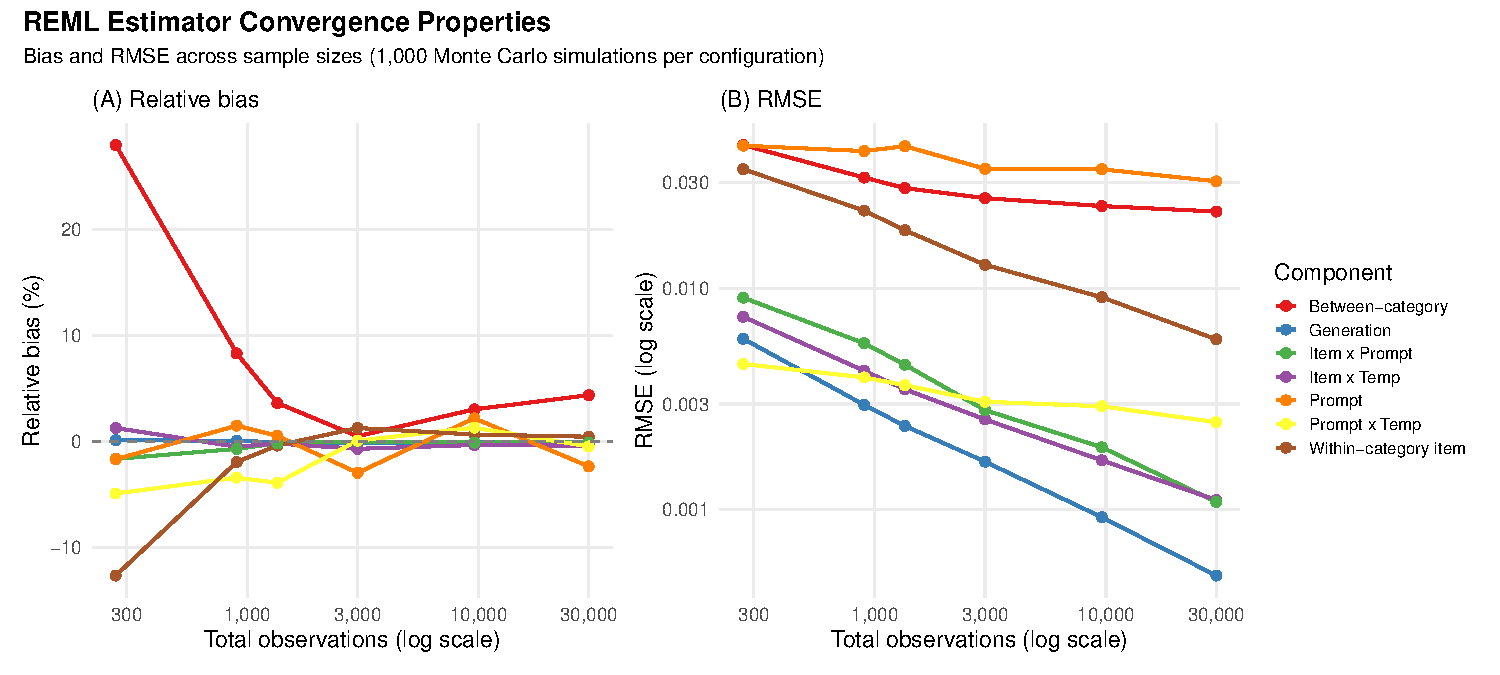
\includegraphics[width=\textwidth]{manuscript_fig1_convergence.pdf}
\caption{REML estimator convergence. (a)~Bias falls below 5\% for all components once total observations exceed 1,000. (b)~RMSE by component across sample sizes, showing monotonic decline. Interaction components ($\sigma^2_{\alpha\phi}$, $\sigma^2_{\alpha\lambda}$) require larger samples for precise estimation than main effects. 1,000 simulations per configuration.}
\label{fig:convergence}
\end{figure}

\subsection{Robustness Studies}\label{si:robustness}

Four studies probe how the variance decomposition and D-study projections degrade under specific assumption violations, and the framework holds up across all four.

\phantomsection\label{si:additivity}
Three-way item$\times$variant$\times$temperature interactions barely move the decomposition. Sweeping their magnitude from 0 to 100\% of the largest two-way component ($N = 50$, $C = 5$, $V = 4$, $H = 3$, $R = 5$) shifts Kendall's $\tau$ on the D-study ranking only from 0.895 to 0.877 at maximum violation, and non-residual components show under 5\% relative bias across all levels.

Per-stratum REML recovers heteroscedastic residuals to within 0.3\% relative bias. With temperature-specific residuals at $\sigma^2_{\epsilon,0} = 0.005$, $\sigma^2_{\epsilon,0.7} = 0.04$, and $\sigma^2_{\epsilon,1.0} = 0.08$, fitting a separate mixed-effects model per temperature via \texttt{lme4::lmer} recovers each within 0.3\% bias. A single homoscedastic \texttt{lmer} fit pools to a weighted average instead, and the \texttt{glmmTMB} dispersion model substantially overestimates residual variance. Non-residual components remain unbiased under all three estimators.

\phantomsection\label{si:small_v}
$\hat{\sigma}^2_\phi$ requires $V \geq 3$ for reliable estimation. Sweeping $V \in \{2, 3, 4, 5, 7, 10\}$ and $\sigma^2_\phi \in \{0, 0.04, 0.10\}$ produces $+4$ to $+5\%$ bias at $V = 2$ and 1 - 4\% at $V \geq 3$ (Figure~\ref{fig:small_k}). A knife-edge test shows directional accuracy collapses to near chance when prompts and replications contribute equally, but recovers when one source clearly dominates.

\begin{figure}[h]
\centering
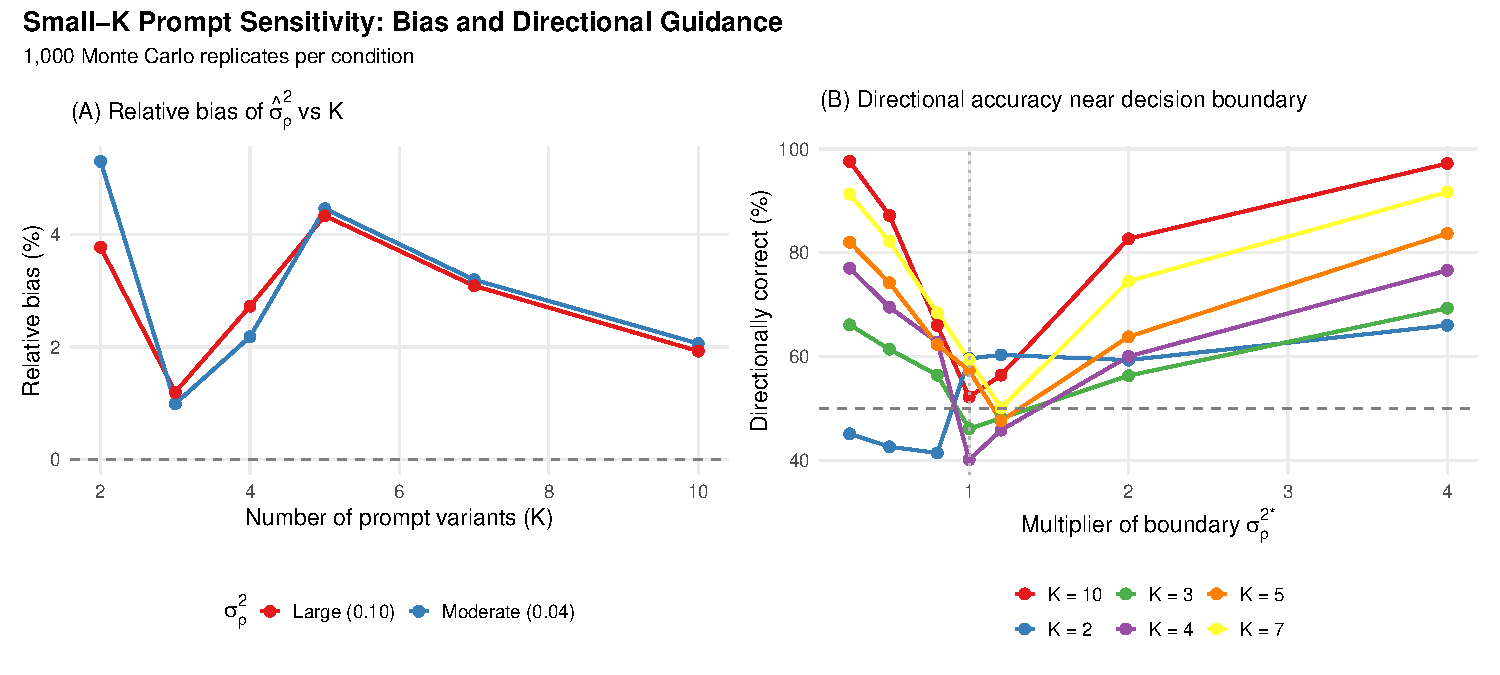
\includegraphics[width=\textwidth]{manuscript_fig2_small_k.pdf}
\caption{Small-$V$ prompt sensitivity estimation. (a)~Relative bias of $\hat{\sigma}^2_\phi$ versus number of prompt variants $V$. At $V\!=\!2$, bias is 4 - 5\%; at $V \geq 3$, bias drops below 4\%, supporting the minimum design recommendation of $V \geq 3$. (b)~Directional accuracy of the D-study recommendation (add prompts vs.\ add replications) near the knife-edge boundary where both interventions yield equal gains. Accuracy exceeds 90\% when one source clearly dominates but drops to near chance at the boundary. 1,000 replicates per condition. Axis label uses $K$ for prompt variants (simulation convention). $K = V$ in main text notation.}
\label{fig:small_k}
\end{figure}

D-study projections transfer imperfectly between model profiles but identify the right top intervention most of the time. Across two profiles (a low-noise frontier model and a high-noise cheaper model), component estimates carry 55 - 59\% relative error when frontier components project to the cheaper profile, and 127 - 154\% in the reverse direction, but the projected top intervention is nonetheless incorrect only 9 - 13\% of the time.

\subsection{D-Study Projection Validation Under Misspecification}
\label{si:dstudy_validation}

We stress-test D-study projections under five scenarios. Scenario 1 is a correctly specified baseline. The other four perturb the DGP along a different axis each: correlated random effects ($\alpha = 2$), non-exchangeable prompt clusters (ratio of 8 between cluster variances), heavy-tailed score residuals (Student-$t$ with df $= 5$), and heterogeneous category $\times$ variant variance (a $0.25\times$ vs.\ $4\times$ ratio across categories). Each scenario draws 1{,}000 Monte Carlo replicates from its DGP. We fit the standard TEE model and compare projected variance components against the truth. The relative bias in the projected variance ranges from $-7.2\%$ (heavy-tailed) to $-0.9\%$ (baseline), with the other three between $-2.3\%$ and $-1.6\%$ (Table~\ref{tab:dstudy_misspec}). All five scenarios produce $|\text{bias}| \leq 8\%$, supporting the framework under the assumption violations tested.

\begin{table}[h]
\centering
\small
\caption{D-study projection bias under five scenarios: one correctly specified baseline and four misspecification conditions (correlated random effects, non-exchangeable prompts, heavy-tailed scores, heterogeneous category interactions). All scenarios produce $|\text{bias}| \leq 8\%$, confirming that D-study projections are stable under the assumption violations tested. $N_\text{sim} = 1,000$.}
\label{tab:dstudy_misspec}
\begin{tabular}{llr}
\toprule
Scenario & Key parameter & Rel.\ bias (\%) \\
\midrule
1. Correct specification & - & $-0.9$ \\
2. Correlated RE & $\alpha = 2$ & $-2.0$ \\
3. Non-exchangeable prompts & ratio $= 8$ & $-1.6$ \\
4. Non-normal scores & df $= 5$ & $-7.2$ \\
5. Heterogeneous category $\times$ variant & 0.25/4$\times$ & $-2.3$ \\
\bottomrule
\end{tabular}
\end{table}

\begin{figure}[h]
\centering
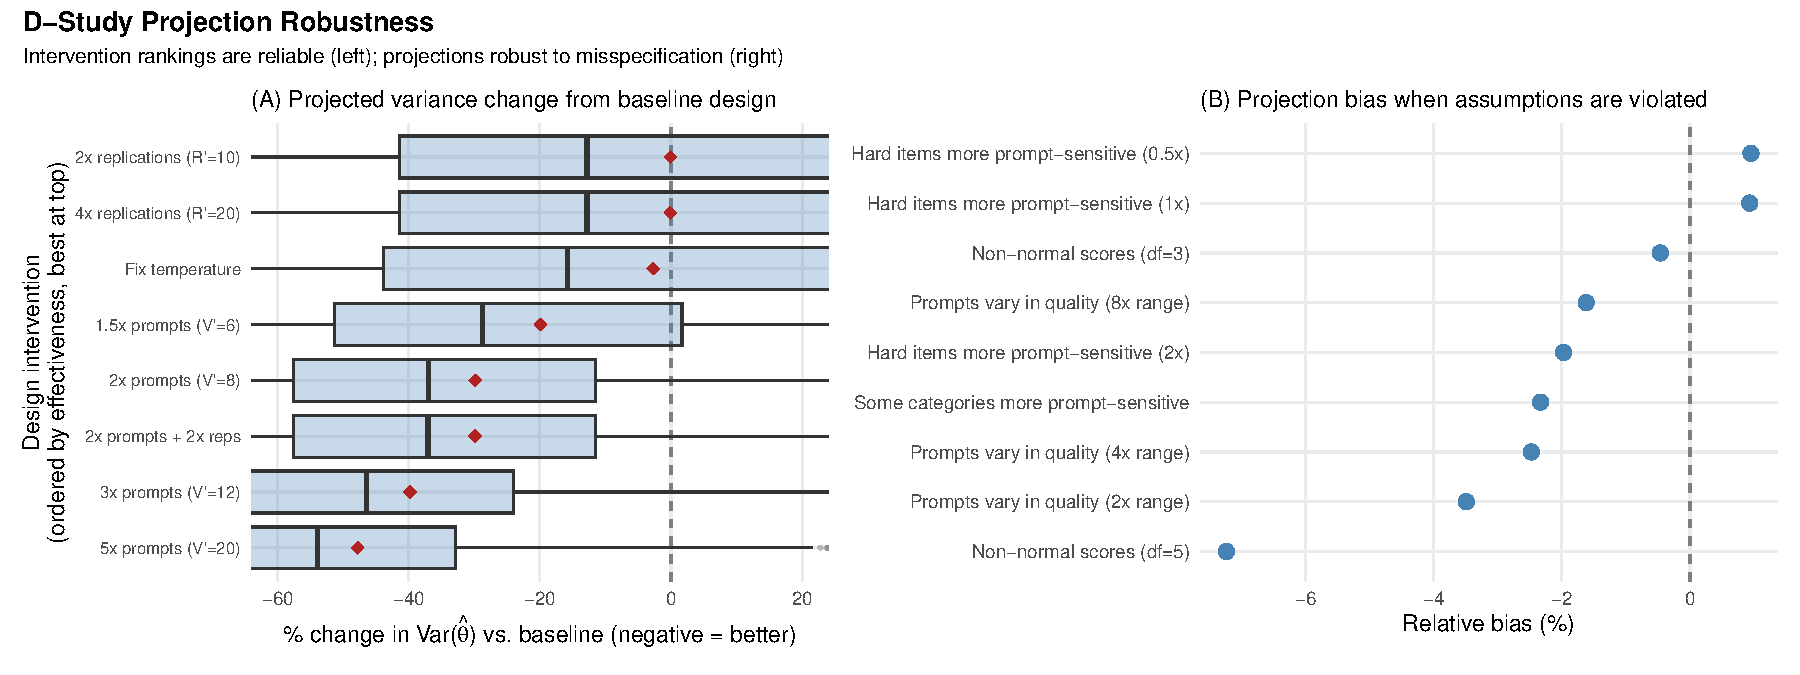
\includegraphics[width=\textwidth]{manuscript_fig3_dstudy.pdf}
\caption{D-study projection validation. (a)~Projected \% change in variance for each intervention (1,000 datasets). Red diamonds: true change. (b)~Projection accuracy under assumption violations, with bias $\leq 8\%$. Details in Section~\ref{si:dstudy_validation}.}
\label{fig:dstudy_robustness}
\end{figure}

\subsection{Scoring Method Recovery Under Judge Heterogeneity}
\label{si:scoring_recovery}

Scoring method is one of the most consequential design choices in LLM evaluation. The TEE decomposition takes scores as input and partitions their variance, but it cannot see upstream of the scoring function, so a D-study built on a variance profile distorted by scoring pathologies will recommend the wrong interventions. Getting the D-study right requires getting the scoring function right first.

Three well-documented LLM judge pathologies degrade absolute rating scales while leaving pairwise comparisons largely intact, and the structural reason is the same for all three. Central tendency compression makes judges cluster ratings near the scale midpoint \citep{esmaeili2025quantitative}, discarding information at the extremes; in pairwise comparison, both items share the same call context, so compression affects both equally and preserves their relative ordering. Low self-consistency means the same item receives different ratings across repeated calls (intra-rater agreement can be as low as $\alpha \approx 0.27$, \citealt{haldar2025roulette}); in pairwise comparison, per-call anchoring noise is additive to both items and cancels in the difference. Scale-use heterogeneity (the rater analog of differential item functioning, \citealt{holland1993differential}) means judges apply different mappings from perceived quality to scale values; pairwise comparison is immune to multiplicative scale differences because the mapping multiplies both items equally and preserves the sign of the difference, though nonlinear differential functioning can still affect comparisons.

Calibrating a shared rubric across heterogeneous raters is infeasible. Fitting pairwise preferences with a Bradley-Terry model sidesteps the scale-calibration problem entirely. Chatbot Arena \citep{chiang2024chatbot} scores models this way for exactly this reason. These pathologies produce reduced discriminability analogous to satisficing in survey research \citep{krosnick1991response}, and pairwise costs more per comparison and is susceptible to position bias.

To verify these arguments empirically, we run a simulation that generates items with known latent quality scores, applies Likert and Bradley-Terry (BT) scoring under identical per-observation noise \citep{peysakhovich2015pairwise}, and sweeps five Likert pathologies: central tendency compression ($\kappa$), per-observation anchoring noise ($\sigma_\text{anchor}$), scale-use heterogeneity ($\sigma_\text{slope}$), nonlinear scale distortion ($\gamma$), and discretization loss (number of scale points). Because both scoring arms receive identical per-observation noise, any pairwise advantage isolates structural properties of the comparison (shared context, immunity to compression and DIF) from noise differentials. Four experiments cross these pathologies: (1) ideal conditions, (2) a 3-way sweep of $\kappa \times \sigma_\text{anchor} \times \sigma_\text{slope}$ (64 conditions), (3) $\kappa \times \gamma \times$ scale points (48 conditions), and (4) a full 5-way crossing (768 conditions).

The simulation confirms the analytical predictions. Under ideal conditions, Likert matches full-budget BT ($\tau \approx 0.835$); under any of the five pathologies, Likert degrades while BT stays stable (Figure~\ref{fig:scoring_recovery}). Central tendency compression is the dominant effect. As $\kappa$ decreases from 1.0 to 0.3, Likert $\tau$ drops from 0.46 to 0.43 while BT stays flat at 0.50. Discretization compounds this. Reducing from continuous scoring to a 3-point scale drops Likert to $\tau = 0.38$. The gap is most dramatic at low prevalence, where binary classification collapses from $\tau = 0.60$ at 50\% prevalence to $\tau = 0.06$ at 0.05\% prevalence while BT remains stable ($\tau \approx 0.73$ at 0.05\%). This prevalence sensitivity is directly relevant to safety evaluation, where high safe rates (94\% in the main-text demonstration) push binary classifiers into the unreliable regime.

Three decision rules follow from the simulation and the measurement-theory literature. When LLM judges are well calibrated and use fine scales (7+ points, $\kappa > 0.7$), Likert and pairwise scoring recover rankings comparably, and Likert costs roughly one-third as much per item, making it the default choice in this regime. When judge calibration is poor or unknown, or the scale is coarse (3 - 5 points), pairwise comparison provides substantial stability under compression, anchoring noise, and scale-use heterogeneity, with the 3$\times$ cost premium buying that stability. For binary outcomes at low prevalence, pairwise dominates because binary classification accuracy degrades sharply below 5\% prevalence while BT remains stable across all prevalence levels tested (0.05 - 50\%).

These rules assume adequate position-bias mitigation. The empirical demonstration found a 66\% B-rate across the three judges, and order-counterbalancing combined with a position covariate was needed to bring residual position bias within acceptable bounds (SI Appendix, Section~\ref{si:pilot}). Scoring method is therefore a design choice that simulation and measurement theory together inform.

\begin{figure}[h]
\centering
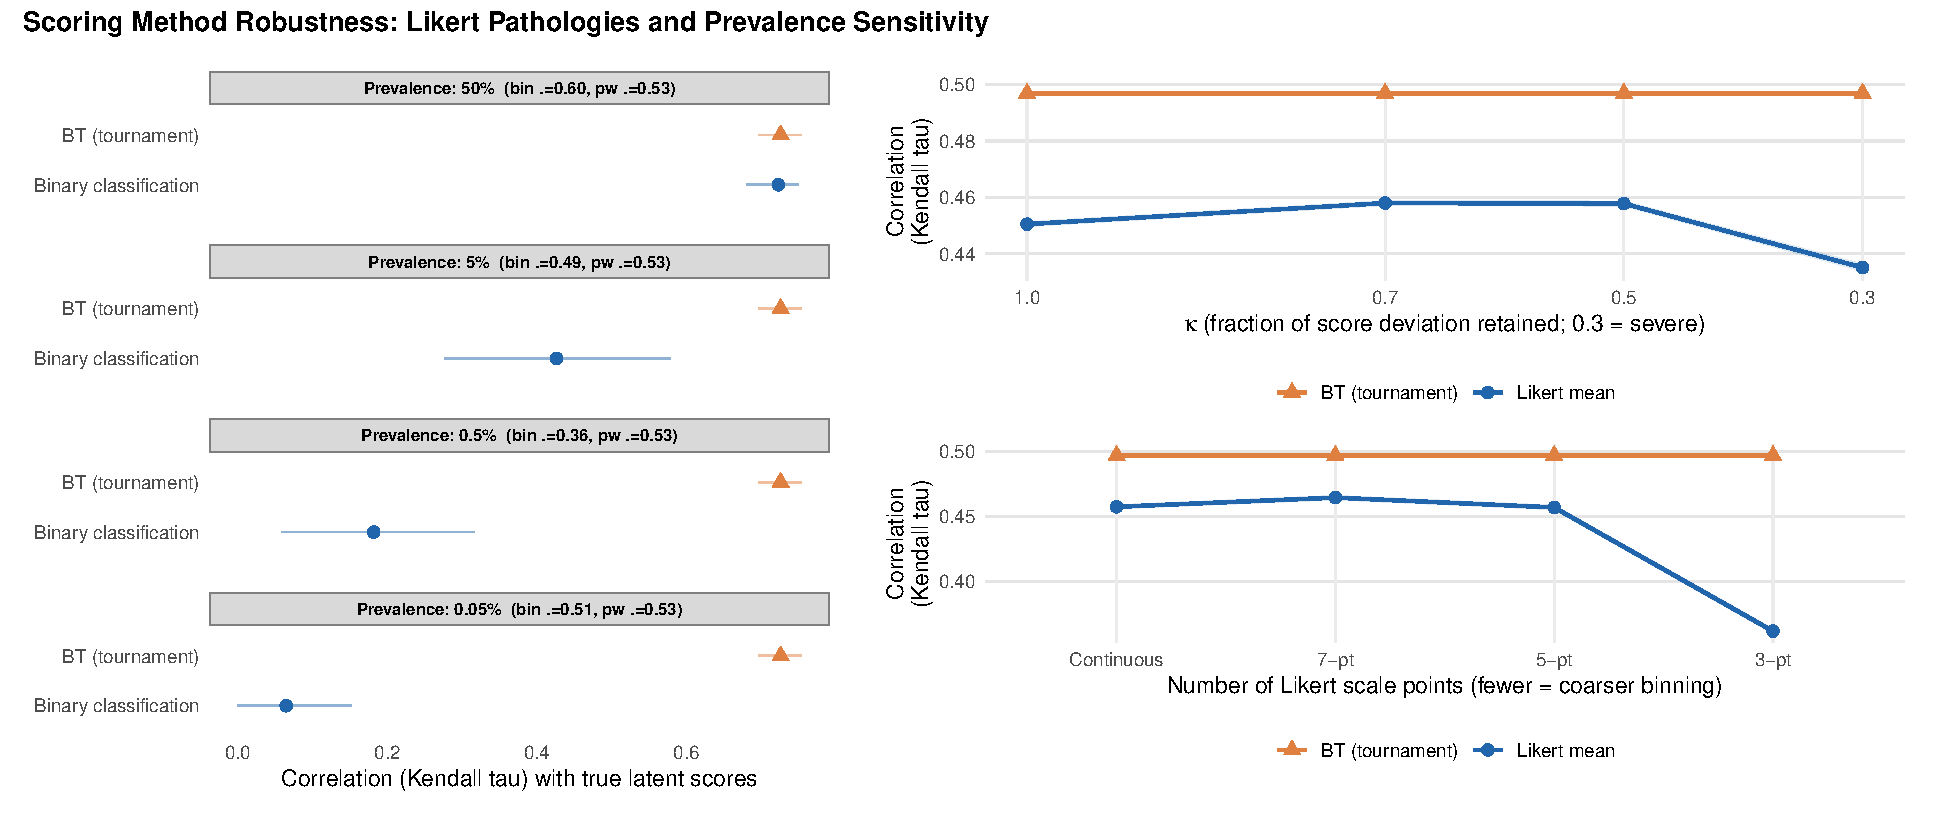
\includegraphics[width=\textwidth]{manuscript_fig_scoring_compound.pdf}
\caption{BT pairwise scoring is stable under Likert pathologies. Left: at low prevalence, binary classification collapses while BT remains stable. Upper right: central tendency compression ($\kappa$) degrades Likert ranking recovery, while BT is unaffected. Lower right: coarser Likert scales (fewer points) reduce recovery, while BT is invariant to discretization. The full simulation sweeps five pathologies ($\kappa$, $\sigma_\text{anchor}$, $\sigma_\text{slope}$, nonlinear $\gamma$, discretization). This figure shows the three with the largest effects. $N_\text{sim} = 200$.}
\label{fig:scoring_recovery}
\end{figure}

\subsection{Variance Underestimation When Pipeline Factors Are Omitted}\label{si:underestimation_sim}

The main text (Figure~\ref{fig:underestimation}) shows that naive CIs fail when the fitted model omits random effects for pipeline factors that contribute variance. This section details the six scenarios behind that result and traces how coverage degrades as design-side components are omitted from the fitted model.

The DGP sets the pipeline components to comparable magnitudes, so that each scenario captures a visible slice of the variance (Table~\ref{tab:underestimation_dgp}). It illustrates the mechanism and is not calibrated to any benchmark. The full factorial uses $V = 4$ prompt variants, $H = 3$ temperatures, $M = 3$ judges, and $R = 8$ replications.

\begin{table}[h]
\centering
\small
\caption{DGP parameters for the variance underestimation simulation (\texttt{analysis/04g2\_sim\_underestimation\_balanced.R}). Temperature and judge enter as fixed levels; every other component is a random-effect variance.}
\label{tab:underestimation_dgp}
\begin{tabular}{lll}
\toprule
\textbf{Component} & \textbf{Value} & \textbf{Notes} \\
\midrule
$\sigma^2_\alpha$ (item)            & 0.10 & \\
$\sigma^2_\phi$ (prompt)            & 0.04 & \\
$\tau$ (temperature levels)         & $\{-0.20, 0, 0.20\}$ & $\mathrm{pop\_var}(\tau) = 0.027$ \\
$\lambda$ (judge levels)            & $\{-0.20, 0, 0.20\}$ & $\mathrm{pop\_var}(\lambda) = 0.027$ \\
$\sigma^2_{\alpha\phi}$ (item $\times$ prompt) & 0.04 & \\
$\sigma^2_{\alpha\tau}$ (item $\times$ temperature) & 0.03 & \\
$\sigma^2_{\alpha\lambda}$ (item $\times$ judge) & 0.04 & \\
$\sigma^2_{\phi\tau}$, $\sigma^2_{\phi\lambda}$, $\sigma^2_{\tau\lambda}$ & 0.02 & design $\times$ design \\
$\sigma^2_\epsilon$ (cell-level)    & 0.04 & constant across replicates within a cell \\
$\sigma^2_\rho$ (replicate)         & 0.10 & within-cell replicate noise \\
\bottomrule
\end{tabular}
\end{table}

Six scenarios sample from this factorial and fit progressively richer \texttt{lmer} models (Table~\ref{tab:underestimation_scenarios}). Scenario A is the naive baseline. It samples one observation per item at a randomly chosen (prompt, temperature, judge) configuration and reports $\mathrm{SE} = s/\sqrt{N}$. Scenarios B, C, and D then add prompt-variant, judge, and temperature random effects in turn, sampling the corresponding factor in full. Scenario E adds the design-by-design interactions. Scenario F fits cell means with the item interactions as well, which separates the cell-level term $\sigma^2_\epsilon$ from replicate noise.

\begin{table}[h]
\centering
\small
\caption{Scenarios A - F progressively enrich the fitted random-effects model. Each row indicates the factorial dimensions the scenario samples, the random effects it adds, the variance it then captures, and what remains uncaptured.}
\label{tab:underestimation_scenarios}
\resizebox{\linewidth}{!}{%
\begin{tabular}{lllll}
\toprule
\textbf{Scenario} & \textbf{Sampled} & \textbf{Adds} & \textbf{Captures} & \textbf{Misses} \\
\midrule
A (naive) & $V{=}1, M{=}1, H{=}1, R{=}1$ & $s/\sqrt{N}$ & - & all design-side \\
B         & $V{=}4, M{=}1, H{=}1, R{=}8$ & \texttt{(1|variant)}        & $\sigma^2_\phi$    & $\tau, \lambda$, interactions \\
C         & $V{=}4, M{=}3, H{=}1, R{=}8$ & + \texttt{(1|judge)}        & + $\lambda$ & $\tau$, interactions \\
D         & $V{=}4, M{=}3, H{=}3, R{=}8$ & + \texttt{(1|temp)}         & + $\tau$  & interactions \\
E         & same data as D               & + \texttt{(1|variant:judge), (1|variant:temp), (1|temp:judge)} & + design $\times$ design & item $\times$ design, $\sigma^2_\epsilon$ \\
F         & cell means of D's data       & + \texttt{(1|item:variant), (1|item:judge), (1|item:temp)} & + item $\times$ design, $\sigma^2_\epsilon$ & - \\
\bottomrule
\end{tabular}}
\end{table}

The point estimate in every scenario is the mean of the sampled observations. The SE is $\sqrt{\text{Var}(\hat\beta_0)}$ from the fitted \texttt{lmer}, except for A, which uses $s/\sqrt{N}$. A fit that exceeds a 300-second timeout falls back to the oracle SE computed from the true variance components under that scenario's model; this happened in 28 of the 1,000 Scenario E replicates at $N = 400$ and in no other cell. All six scenarios are evaluated at $N \in \{25, 50, 100, 200, 400\}$ with 1,000 Monte Carlo replicates per cell.

The six scenarios produce a coverage staircase, with each fit capturing more of the design-side variance. Scenario A captures nothing. Its SE is the naive $s/\sqrt{N}$ and shrinks with sample size, while the bias from the single (prompt, temperature, judge) configuration stays constant, so coverage falls from 42\% at $N = 25$ to 11\% at $N = 400$. Scenario B adds prompt-variant random effects and reaches 56 - 64\% coverage, with the unmodeled judge and temperature offsets keeping it well below nominal. Scenario C adds judges and reaches 86 - 89\%, limited by the remaining temperature offset. Scenarios D, E, and F capture every design-side component and cover at 99 - 100\%, above nominal, with SEs 9 - 19\% larger than the oracle SE. E and F have identical coverage at this design; F's advantage is that it separates the cell-level term $\sigma^2_\epsilon$ from replicate noise, which matters when $\sigma^2_\epsilon$ is large.

\begin{figure}[h]
\centering
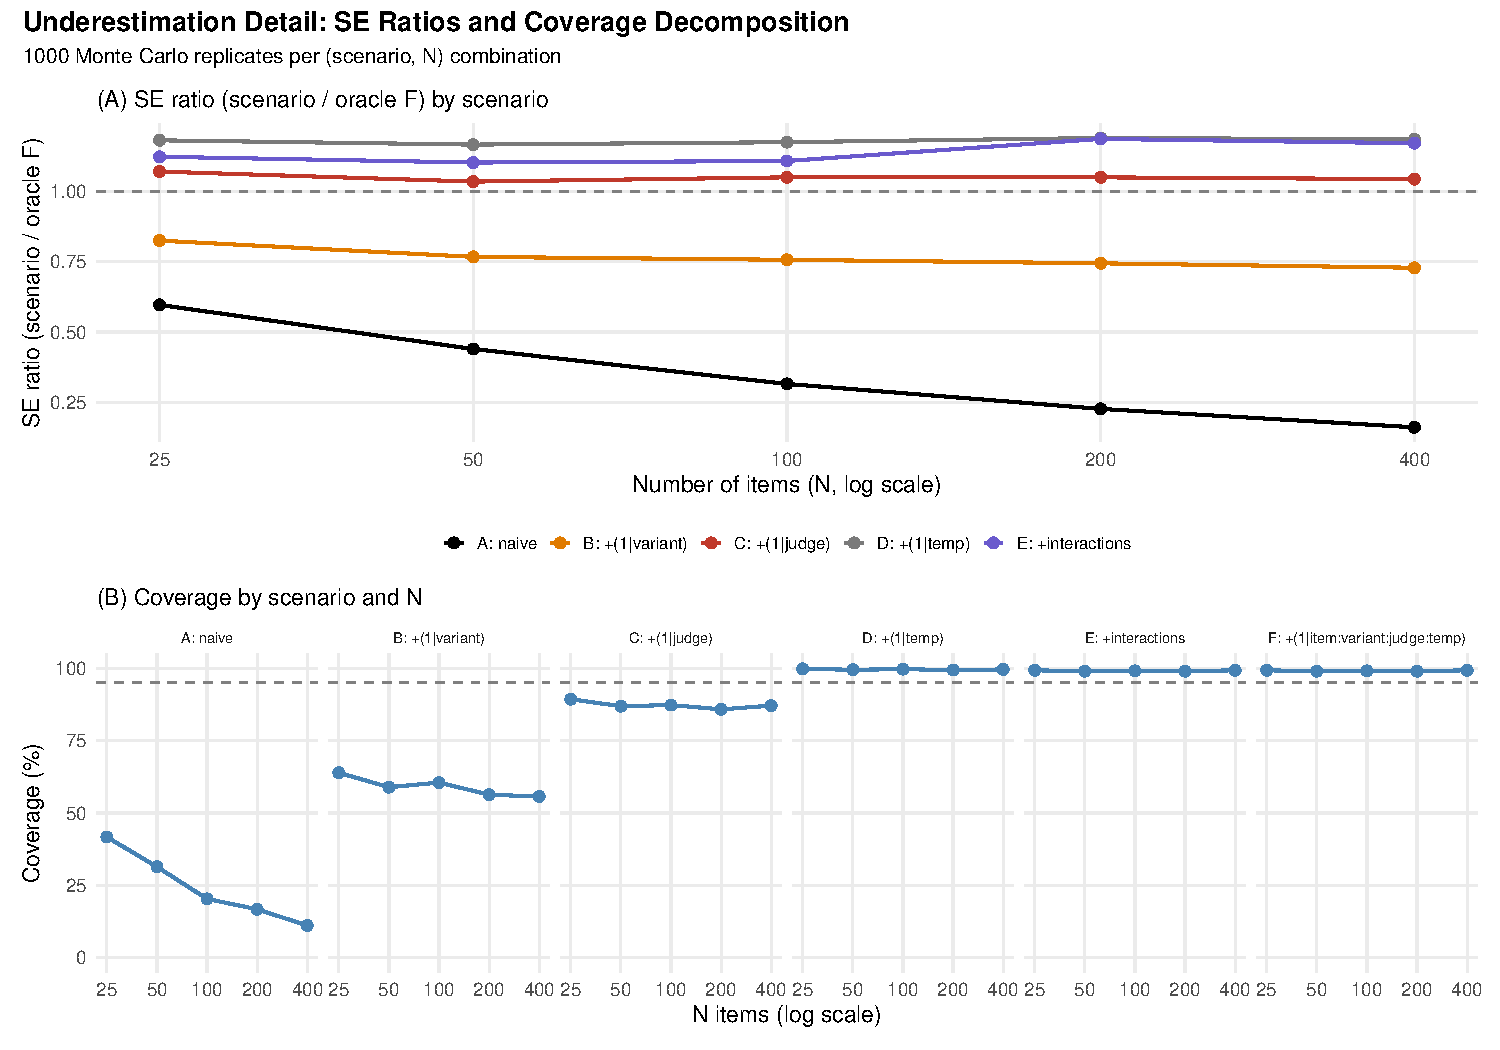
\includegraphics[width=\textwidth]{manuscript_fig_underestimation_detail_v2.pdf}
\caption{Naive 95\% CIs lose coverage as sample size grows because the SE shrinks while the bias from omitted pipeline factors stays constant. Panel (a) plots each scenario's SE relative to the oracle SE of the full model, with the naive Scenario A about $6\times$ smaller at $N = 400$. Panel (b) plots 95\% CI coverage versus $N$ for the six scenarios, showing how each added random effect (prompt in B, judge in C, temperature in D, interactions in E and F) closes one more component of the omitted variance and lifts coverage toward nominal. $N \in \{25, 50, 100, 200, 400\}$; $N_\text{sim} = 1,000$.}
\label{fig:underestimation_detail}
\end{figure}


\subsection{Latent Item Ambiguity}\label{si:latent_ambiguity}

This simulation builds an even harsher misspecification: per-item variance heterogeneity driven by a latent ambiguity score, combined with a sparse 3-way interaction concentrated in the ambiguous tail. The motivating concern is that earlier robustness simulations addressed additivity violations (Section~\ref{si:additivity}) and correlated random effects (Section~\ref{si:dstudy_validation}) in isolation. When both arise jointly from the same latent property of the item, do D-study projections still reflect the truth?

The DGP draws a per-item ambiguity score $z_i \sim N(0, 1)$ and scales that item's item$\times$prompt and item$\times$judge variances by $1 + \gamma z_i^2$. Higher-$z_i$ items therefore swing more under prompt and judge variation. Items with $z_i > 1$ (roughly 16\% of the population) additionally carry a 3-way item$\times$prompt$\times$judge interaction with variance $0.01$, so prompt and judge effects compound nonadditively for the most ambiguous items. We sweep $\gamma$ over $\{0, 0.5, 1, 2\}$. The endpoints anchor the experiment: $\gamma = 0$ is correct specification, $\gamma = 2$ triples interaction variance one SD above the mean.

We sample a small factorial of $N = 30$ items across $C = 5$ categories, $V = 3$ prompts, $H = 2$ temperatures, $M = 3$ judges, and $R = 3$ replications, totaling 1,620 cells per fit. The TEE specification carries the two-way interactions only; the 3-way interaction and the latent heterogeneity remain outside the model.

CI coverage holds at 89 - 91\% across all four $\gamma$ settings, against the 95\% nominal under such a small $N$. The worst component-level relative bias is below 9\% and D-study intervention rankings agree perfectly with the truth (Spearman $\rho = 1.0$) across 1{,}000 simulations per setting. Breakdown by $\gamma$ in Table~\ref{tab:latent_ambiguity}.

\begin{table}[h]
\centering
\small
\caption{TEE stability under latent item ambiguity. $\gamma$ controls the strength of ambiguity-driven dependence between item difficulty and interaction variances, with sparse 3-way interactions for ambiguous items ($z_i > 1$). CI coverage does not degrade, component bias stays below 9\%, and D-study intervention rankings are preserved exactly across all ambiguity levels. $N_\text{sim} = 1,000$.}
\label{tab:latent_ambiguity}
\begin{tabular}{llrrr}
\toprule
$\gamma$ & Label & Coverage (\%) & Max $|\text{rel.\ bias}|$ (\%) & D-study $\rho$ \\
\midrule
0   & Baseline    & 90.5 & 8.8 & 1.00 \\
0.5 & Mild        & 88.7 & 6.7 & 1.00 \\
1   & Moderate    & 90.3 & 3.4 & 1.00 \\
2   & Strong      & 91.2 & 6.0 & 1.00 \\
\bottomrule
\end{tabular}
\end{table}

Why does this work? \texttt{lmer} estimates \emph{marginal} variance components, namely the population averages over items, not per-item variances. With each item's item$\times$prompt component scaled by $1 + \gamma z_i^2$, the population average of the scaling is $E[1 + \gamma z_i^2] = 1 + \gamma$, giving a marginal item$\times$prompt variance of $(1 + \gamma)\sigma^2_{\alpha\phi}$, which is what the estimator returns. The sparse 3-way interaction concentrates in a small fraction of items, lands in the residual bucket, and inflates $\hat{\sigma}^2_\epsilon$ slightly. The two-way components stay intact.

Untested scenarios include multimodal residuals (e.g., from a mixture of refusals and compliance), extreme base rates (above 0.9 or below 0.1), unbalanced designs with missing cells, post-hoc model specification search, and nonlinear temperature effects.


%% ============================================================================
%% SI SECTION 4: MULTI-TURN AND MULTI-AGENT EXTENSIONS
%% ============================================================================

\clearpage

\section{Multi-Turn and Multi-Agent Extensions}
\label{si:extensions}

\subsection{Multi-Turn Extension}

The single-turn DGP extends to multi-turn evaluation when each turn's score depends on the prior conversation. Adding a turn index $t$ and a turn-conditional mean $\mu_t(\mathbf{h}_{<t})$ for the expected score given history $\mathbf{h}_{<t}$ yields\footnote{In this subsection $\eta(t)$ denotes the hazard rate and $\mathbf{h}_{<t}$ denotes conversation history, distinct from the subscript $h$ used for temperature in the main DGP.}
\begin{equation}
Y_{t,ivhm}^{(r)} = \mu_t(\mathbf{h}_{<t}) + \alpha_i + \phi_v + \tau_h + (\alpha\phi)_{iv} + \epsilon_{t,ivhm} + \rho_{t,ivhm}^{(r)}.
\end{equation}
The pipeline-side variance components keep their single-turn interpretations because they describe how the evaluation is computed, not how the conversation evolves. The multi-turn structure enters through $\mu_t(\mathbf{h}_{<t})$, which drifts as the model conditions on accumulating context.

Safety evaluation often asks at what turn the model first crosses a safety threshold $\theta^*$, which maps onto a survival framing with hazard rate
\begin{equation}
\eta(t) \approx \Phi\!\left(\frac{\mu_t(\mathbf{h}_{<t}) - \theta^*}{\sqrt{\text{TEE}_t}}\right).
\end{equation}
This Gaussian-tail approximation treats $\eta(t)$ as the probability that a Gaussian score with mean $\mu_t(\mathbf{h}_{<t})$ and variance $\text{TEE}_t$ exceeds the threshold $\theta^*$. Pipeline-level variance therefore inflates the hazard at any threshold, so the same components that distort single-turn CIs also amplify multi-turn safety risk. Full integration with Cox proportional hazards models \citep{cox1972regression} for time-varying covariates is beyond the current scope. Existing empirical work supports the framing. \citet{weng2025footinthedoor} document harmfulness scores increasing across turns under foot-in-the-door attacks, consistent with $\mu_t(\mathbf{h}_{<t})$ drifting upward as context accumulates. \citet{li2025timetoincon} fit hazard models to multi-turn LLM interactions and find that hazard rates depend on temperature, supporting the inclusion of $\tau_h$ in the multi-turn DGP.

\subsection{Multi-Agent Extension}

Now suppose the pipeline runs $A$ agents in parallel on the same item, $Y_1,\ldots,Y_A$, and reports their mean $\bar Y$. Writing out the variance of that mean gives
\begin{equation}
\Var(\bar{Y}) = \frac{1}{A^2}\left[\sum_{a=1}^{A} \text{TEE}_a + \sum_{a \neq a'} \Cov(Y_a, Y_{a'})\right].
\end{equation}
We get the usual $1/A$ shrinkage in each agent's TEE, which is what makes ensembling worth its budget. But the off-diagonal covariances do not vanish whenever agents share training data or share scoring rubrics; correlated errors add to the sum and chew into the shrinkage. We have already met this special case: a multi-judge panel scoring one response, with judges in place of agents.

When agents are chained instead, agent $A$ inherits its input from agent $A-1$. The variance of the final score factorizes via the law of total variance,
\begin{equation}
\Var(Y_A) = \E[\Var(Y_A \mid Y_{A-1})] + \Var(\E[Y_A \mid Y_{A-1}]).
\end{equation}
We read the conditional-variance piece as agent $A$'s own contribution and the variance-of-conditional-expectation piece as what got pushed through from upstream. Recursing this back through the chain attributes total variance to each agent's local share plus everything it inherited \citep{duan2025uprop}. \citet{kim2025scaling} found that 17.2$\times$ error amplification for independent agent topologies, versus 4.4$\times$ for centralized ones, which makes architecture a TEE design choice with leverage similar to judge or prompt selection.



\clearpage

\section{GLMM Robustness Check}
\label{si:glmm}

Binary outcomes in the main text use a linear probability model \citep[LPM,][]{angristpischke2009}. The LPM residuals for binary data are heteroscedastic, raising the question of whether the variance-component shares reported in the main text are link-function artifacts. To check, we refit the three binary decompositions with a logit link via \texttt{lme4::glmer(family = binomial)} \citep{bates2015lme4} and compare the GLMM shares with the LPM shares used in the main text.

\begin{table}[ht]
\centering
\caption{LPM vs.\ GLMM Var($\hat\theta$) decomposition for the three binary benchmarks (pairwise ideology, safety classification, MMLU). LPM shares are on the probability scale; GLMM shares are on the logit scale, so absolute SE values are not directly comparable, but component rankings are. For the GLMM, the level-1 residual is fixed at $\pi^2/3$ following the logistic-link convention \citep{nakagawa2010repeatability}. All three fits include the cell-level random effect. For MMLU the model layer is the system under test (SUT) rather than a judge. The SUT row plays the same role as ``judge model'' in the other two benchmarks. Spearman rank correlations between LPM and GLMM shares are $\rho = 0.99$ (pairwise), $0.91$ (safety), and $0.95$ (MMLU), confirming that the dominant components are not LPM artifacts.}
\label{tab:glmm_comparison}
\footnotesize
\begin{tabular}{lrrrrrr}
\toprule
& \multicolumn{2}{c}{\textbf{Pairwise (\%)}} & \multicolumn{2}{c}{\textbf{Safety (\%)}} & \multicolumn{2}{c}{\textbf{MMLU (\%)}} \\
\cmidrule(lr){2-3} \cmidrule(lr){4-5} \cmidrule(lr){6-7}
\textbf{Component} & \textbf{LPM} & \textbf{GLMM} & \textbf{LPM} & \textbf{GLMM} & \textbf{LPM} & \textbf{GLMM} \\
\midrule
Judge / SUT model ($\sigma^2_\lambda$, sensitivity) & 68.4 & 50.9 & 43.8 & 70.7 &  6.7 &  7.6 \\
Within-category item ($\sigma^2_\delta$)            &  7.6 & 13.7 & 20.8 & 11.4 & 72.2 & 71.4 \\
Prompt ($\sigma^2_\phi$)                            &  0.4 &  0.4 &  0.0 &  0.0 &  0.4 &  1.3 \\
Item $\times$ judge / SUT ($\sigma^2_{\alpha\lambda}$) &  1.9 &  1.9 & 16.7 &  4.3 & 10.5 &  5.2 \\
Prompt $\times$ judge / SUT ($\sigma^2_{\phi\lambda}$) &  0.1 &  0.0 & 12.4 &  7.9 &  1.3 &  4.4 \\
Position ($\sigma^2_\pi$, sensitivity)              & 20.9 & 32.7 & -    & -    & -    & -    \\
Between-category ($\sigma^2_\kappa$)                &  0.2 &  0.1 &  4.9 &  4.7 &  7.7 &  9.6 \\
Other ($\leq$1\%)                                   &  0.5 &  0.3 &  1.4 &  1.0 &  1.2 &  0.6 \\
\bottomrule
\end{tabular}
\end{table}

The decomposition holds up under the logit link in all three benchmarks. The same component dominates in each case (judge model on pairwise and safety, within-category item heterogeneity on MMLU), and rank correlations are near-perfect ($\rho = 0.99$ pairwise, $0.91$ safety, $0.95$ MMLU). The GLMM amplifies judge-model dominance for safety from 43.8\% (LPM) to 70.7\% (GLMM), because small probability-scale gaps between judges become large logit-scale gaps at the 94\% safe base rate. On MMLU, at the 84.5\% correct base rate, item heterogeneity leads under both links (72.2\% LPM, 71.4\% GLMM), and the three prompt terms stay small on both scales (2.7\% and 6.1\%). We keep the LPM in the main text because its components live on the probability scale and read off as percent-of-variance directly; the GLMM serves here only as the link-function robustness check.



\clearpage

\section{Ideology Scoring Comparison: Likert vs Pairwise}
\label{si:scoring_comparison}

Applied to the same domain under a matched protocol, Likert and pairwise scoring produce qualitatively different variance profiles with different optimization implications.\footnote{An initial pairwise run used a naive prompt (forced A/B, no CoT) and an older judge set (GPT-4o, Gemini~2.0~Flash, Claude~Haiku~4.5). That run was dominated by recency bias (Haiku selected the second response 91\% of the time regardless of content, GPT-4o 70\%, Gemini 38\%), so the raw decomposition attributed 20.7\% of variance to a ``judge main effect'' that was really position bias. Recoding via \texttt{true\_order} collapses this spurious main effect to 0.2\% but migrates the bias noise into item$\times$judge interaction (which rises to 54.7\%), since Haiku's near-random content signal becomes item-level disagreement after recoding. The naive pairwise data is archived. The reference pairwise pipeline described above uses the CoT protocol and a judge set chosen for lower recency bias. A parallel re-run of the Likert pipeline with the matched CoT protocol and matched judges (archiving the earlier naive-Likert run alongside) keeps the scoring-method comparison clean, with the two pipelines now differing only in the rating format.} Four frontier LLMs (Claude~Opus~4.5, GPT-5.1, DeepSeek~Chat~v3.1, Grok~4.1~Fast) generated free-text responses to prompts drawn from five ideology dimensions. A common judge panel and prompt protocol then scored each response under either a 1 - 5 Likert scale or a forced pairwise A/B comparison.

Both pipelines use a chain-of-thought (CoT) prompt with a content-markers reasoning step, an explicit instruction not to let presentation order or prompt wording bias the decision, and a structured JSON output. The judges are \texttt{openai/gpt-oss-120b}, \texttt{google/gemini-2.0-flash-001}, and \texttt{deepseek/deepseek-chat-v3.1}, with each cell replicated 3 times at 3 temperatures (0, 0.7, 1.0) across 5 paraphrased prompt variants. The Likert pipeline calls 150~items $\times$ 5~variants $\times$ 3~temperatures $\times$ 3~judges $\times$ 3~replications $= 20,250$ times. The pairwise pipeline judges the same 150 item-pairs in both orderings (listed + swapped), and recodes the raw A/B outcome to \texttt{model\_a\_wins} using the item-creation randomization (\texttt{true\_order}) to remove any residual position bias. The pairwise design is also 20,250 calls.

\begin{figure}[htbp]
\centering
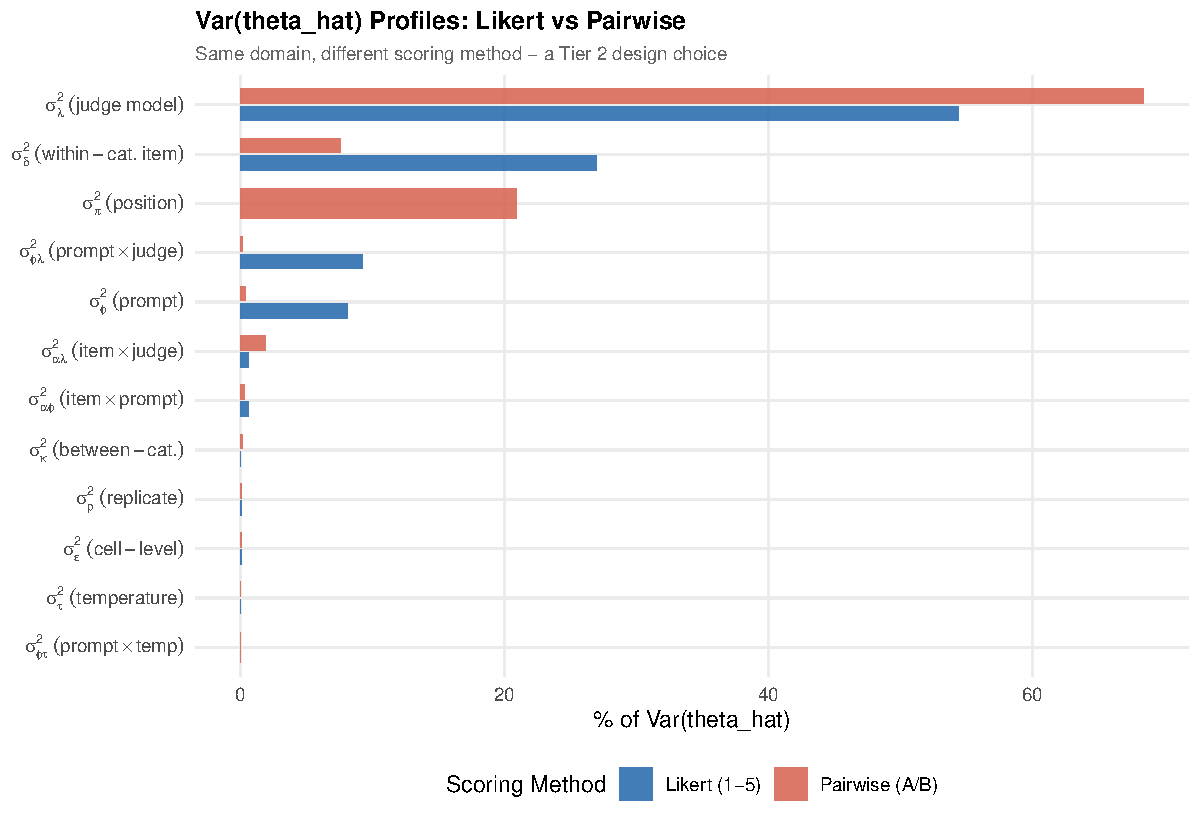
\includegraphics[width=\linewidth]{fig2_scoring_comparison.pdf}
\caption{Judge-model variance dominates both ideology pipelines, but the secondary rankings differ. After judges, Likert is dominated by item heterogeneity and pairwise by position bias, a factor with no Likert analogue. Operational design: $N{=}150$, $V{=}5$, $M{=}3$, $H{=}3$, $R{=}3$ (pairwise also crosses $P{=}2$ position orderings).}
\label{fig:variance_comparison}
\end{figure}

Judge-model design sensitivity tops both decompositions: 54.4\% under Likert and 68.4\% under pairwise. The secondary structure diverges. The Likert ranking continues with within-category item heterogeneity (26.9\%), prompt$\times$judge (9.3\%), and prompt main effect (8.1\%). Pairwise reshuffles. The position factor recoded from listed and swapped orderings via \texttt{true\_order} contributes 20.9\% on its own, within-category item heterogeneity drops to 7.6\%, and item$\times$judge falls to 1.9\%. The two formats trade pathologies. Pairwise avoids compression, anchoring noise, and scale-use heterogeneity \citep{esmaeili2025quantitative, haldar2025roulette, holland1993differential}; Likert pays nothing for position bias. We document the resulting recovery curves in Section~\ref{si:scoring_recovery}: pairwise BT stays stable as those Likert pathologies bite, with binary scoring collapsing at low prevalence ($\tau = 0.06$) where BT still works ($\tau = 0.73$, Figure~\ref{fig:scoring_recovery}).

Despite the different variance profiles, both D-study prescriptions converge on judge variance as the key lever. %Adding judges produces the largest single variance reduction in both formats because $\sigma^2_\lambda/M$ enters with divisor $M$ alone.
Adding items, prompts, or replications buys little marginal precision once their respective terms are well-averaged at $N = 150$, $V = 5$, $R = 3$. Full per-method D-study projections appear in Figures~\ref{fig:dstudy_likert} and~\ref{fig:dstudy_pairwise}.

A separate sanity check explains why pairwise replicate noise is so large. A Claude~Sonnet~4.5 judge with a CoT prompt that \emph{allowed} a TIE option was run on all 150 pairwise items in both orderings. Inter-order consistency was 100\% (every item's listed and swapped judgments either inverted cleanly or both returned TIE), confirming zero position bias. Sonnet returned TIE on 84.7\% of items, so only 23 of 150 pairs carried a clear ideological preference. On those 23 distinguishable items, directional agreement with the three CoT pairwise judges was high (GPT-4o 91\%, Gemini 87\%, Haiku 61\%). The 85\% TIE rate explains why so much pairwise variance lands in $\sigma^2_\rho$ and $\sigma^2_\epsilon$. When forced to pick a side on pairs that are genuinely similar, judges in a forced choice scoring regime produce content-random noise that accumulates within and across cells. The Likert pipeline avoids this failure mode because the 1 - 5 scale permits a centrist rating for ambiguous content.



\clearpage

\section{Pilot Study Details}
\label{si:pilot}

TEE is most useful when researchers can plan a full factorial pipeline from cheap pilot data. This section validates that pilot-scale variance estimates recover the qualitative D-study conclusions of a full run, so a small pilot suffices for design choices that the full pipeline then confirms quantitatively.

We use the Likert ideology demonstration (150 items, 5 prompt variants, 3 temperatures, 3 judges, 3 replications; 20,250 calls) as the testbed. A 30-item, 3-variant subset of the full-run data stands in for the pilot, and we compare its D-study projections to the full-run results. Because the pilot is a subsample of the same items, this test asks whether small-sample variance estimates translate into accurate D-study projections. It does not test how a pilot drawn from completely different items would generalize.

The pilot recovers the qualitative D-study story. Both pilot and full run identify judge-model design sensitivity and within-category item heterogeneity as the two dominant contributors to $\Var(\hat\theta)$. Quantitative shares shift between the two designs because the divisors differ: the pilot allocates 42.4\% to judge model and 48.6\% to within-category item, while the full run allocates 54.4\% and 27.0\% (the larger $N$ in the full run shrinks $\sigma^2_\delta/N$ faster than $\sigma^2_\lambda/M$ at fixed $M$, raising the judge-model share). A pilot-scale run ($N = 30$, $V = 3$, $H = 3$, $M = 3$, $R = 3$; 2,430 calls) thus recovers the qualitative guidance that a 20,250-call full run confirms quantitatively. Practitioners can treat D-study projections as directional guidance accurate to within 20 - 30\% at pilot scale, with the rank ordering of the top two components stable across designs.

Running a pilot and plugging the estimated components into standard errors yields valid confidence intervals. The underlying variance itself is unchanged. Realizing the precision gains from averaging over multiple prompts and judges requires deploying the full factorial pipeline. Section~\ref{si:checklist} operationalizes these recommendations as a three-tier reporting checklist.

\begin{table}[ht]
\centering
\caption{Variance component estimates for the Likert ideology demonstration (CoT protocol): a 30-item, 3-variant pilot subset ($N\!=\!30$, $V\!=\!3$, $M\!=\!3$, $H\!=\!3$, $R\!=\!3$; 2,430 calls) compared with the 150-item full run ($N\!=\!150$, $V\!=\!5$, $R\!=\!3$; 20,250 calls). The pilot correctly identifies the two dominant components (within-category item and judge-model design sensitivity) and recovers their rank ordering. Quantitative shares shift between pilot and full because the divisors differ across designs. The pilot pools $\sigma^2_\rho$ and $\sigma^2_\epsilon$ into a single ``replicate noise'' row because the small $N$ does not separately identify the cell-level term. Shares of mean variance $\Var(\hat\theta)$ at the indicated pilot and full designs.}
\label{tab:pilot_vc}
\small
\begin{tabular}{lrr}
\toprule
\textbf{Component} & \textbf{Pilot (\% Var$(\hat\theta)$)} & \textbf{Full (\% Var$(\hat\theta)$)} \\
\midrule
Judge model ($\sigma^2_\lambda$, sensitivity) & 42.4 & 54.4 \\
Within-category item ($\sigma^2_\delta$)      & 48.6 & 27.0 \\
Prompt $\times$ judge ($\sigma^2_{\phi\lambda}$) &  5.4 &  9.3 \\
Prompt ($\sigma^2_\phi$)                       &  -   &  8.0 \\
Item $\times$ judge ($\sigma^2_{\alpha\lambda}$) &  2.2 &  0.7 \\
Item $\times$ prompt ($\sigma^2_{\alpha\phi}$)  &  1.3 &  0.6 \\
Replicate noise / cell-level ($\sigma^2_\rho + \sigma^2_\epsilon$) &  0.2 &  0.1 \\
All others                  & $<$0.1 & $<$0.1 \\
\bottomrule
\end{tabular}
\end{table}

An earlier naive-prompt pairwise run (forced A/B, no chain-of-thought, judges GPT-4o / Gemini~2.0~Flash / Claude~Haiku~4.5) was superseded because position bias dominated the outcomes. Judges selected the second response 81\% of the time overall and 92\% for Haiku, and the order-counterbalancing already in place (a randomized \texttt{true\_order} at item creation) did not rescue the result, since the judge outputs index position rather than model preference. Recoding the outcome to \texttt{model\_a\_wins} via \texttt{true\_order} removes the bias from the mean (all three judges converge to $\sim$45\% A-wins), but Haiku's 91\% B-rate means its recoded outputs are mostly noise mapped through random flips. The reference pairwise pipeline (Section~\ref{si:scoring_comparison}) therefore switches to a CoT plus bias-mitigated prompt and a judge set chosen for low recency bias (DeepSeek~Chat~v3.1, Gemini~2.0~Flash, GPT-OSS~120B). The naive pairwise data is archived in the replication materials.

D-study projections translate each variance profile into design recommendations. Figures~\ref{fig:dstudy_likert} and~\ref{fig:dstudy_pairwise} report the projected percentage change in $\Var(\hat{\theta})$ for each single-factor intervention under the two scoring formats. The variance shares those projections build from appear in Figure~\ref{fig:variance_comparison}.

\begin{figure}[ht]
\centering
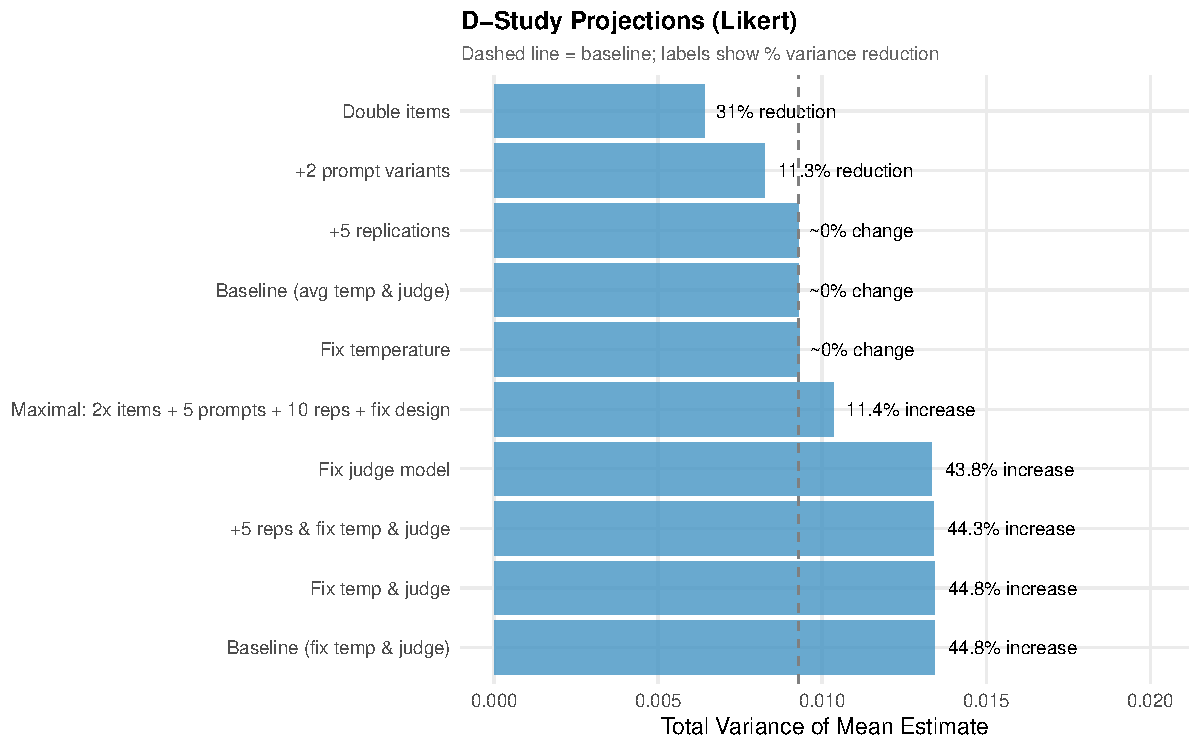
\includegraphics[width=0.9\textwidth]{fig3a_dstudy_likert.pdf}
\caption{Judge averaging is the dominant lever in Likert ideology scoring. Bars show the projected percentage change in $\Var(\hat{\theta})$ for each single-factor intervention. Committing to a single judge inflates variance by 43.8\% because $\sigma^2_\lambda$ (54.4\% of $\Var(\hat\theta)$ at $M = 3$) loses the $1/M$ averaging benefit. Doubling items reduces variance by 31\% by halving the within-category item term ($\sigma^2_\delta$, 26.9\% of $\Var(\hat\theta)$). Adding 2 prompt variants buys 11.3\%. Replications contribute negligibly. Same factorial design as Figure~\ref{fig:variance_comparison}.}
\label{fig:dstudy_likert}
\end{figure}

\begin{figure}[ht]
\centering
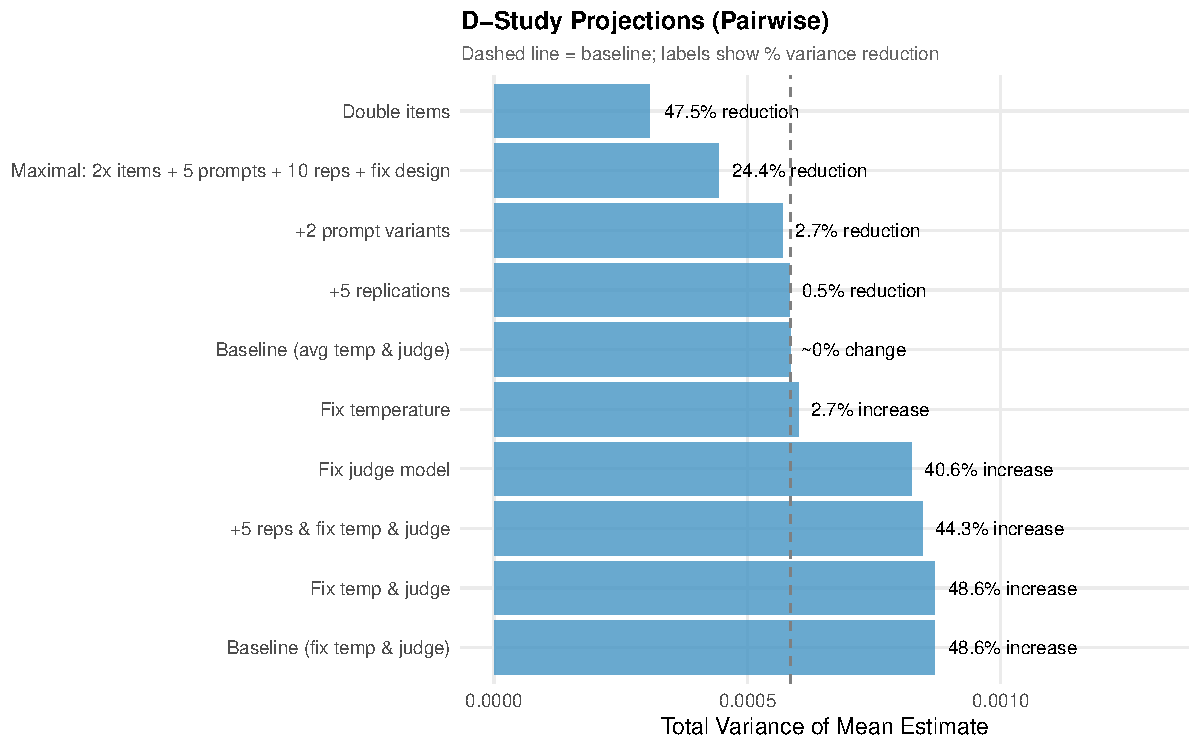
\includegraphics[width=0.9\textwidth]{fig3b_dstudy_pairwise.pdf}
\caption{Doubling items and judge averaging are the dominant levers in pairwise ideology scoring. Bars show the projected percentage change in $\Var(\hat{\theta})$ for each single-factor intervention. Doubling items gives the largest reduction (47.5\%) by halving every $N$-divided term jointly. Committing to a single judge inflates variance by 40.6\% because $\sigma^2_\lambda$ (68.4\% of $\Var(\hat\theta)$ at $M = 3$) loses the $1/M$ averaging benefit. Adding 2 prompt variants buys 2.7\%. Replications contribute negligibly. The position factor ($\sigma^2_\pi$, 20.9\%) is fixed at $P = 2$ in this design and cannot be reduced by averaging. Same factorial design as Figure~\ref{fig:variance_comparison}.}
\label{fig:dstudy_pairwise}
\end{figure}

Cell-level variance is also markedly heterogeneous within each domain. Across five ideology dimensions, $\hat{\sigma}^2_\epsilon$ spans a fourfold range (Figure~\ref{fig:per_category}), so some dimensions produce more variable LLM responses across repeated calls than others. The same heterogeneity is more pronounced in safety classification, where per-category cell-level variance spans more than an order of magnitude (Figure~\ref{fig:safety_catvar}), from $\hat{\sigma}^2_\epsilon = 0.001$ for specialized advice to $\hat{\sigma}^2_\epsilon = 0.033$ for sex crimes. This heterogeneity motivates the heteroscedastic extension (Section~\ref{si:heteroscedastic}).

\begin{figure}[ht]
\centering
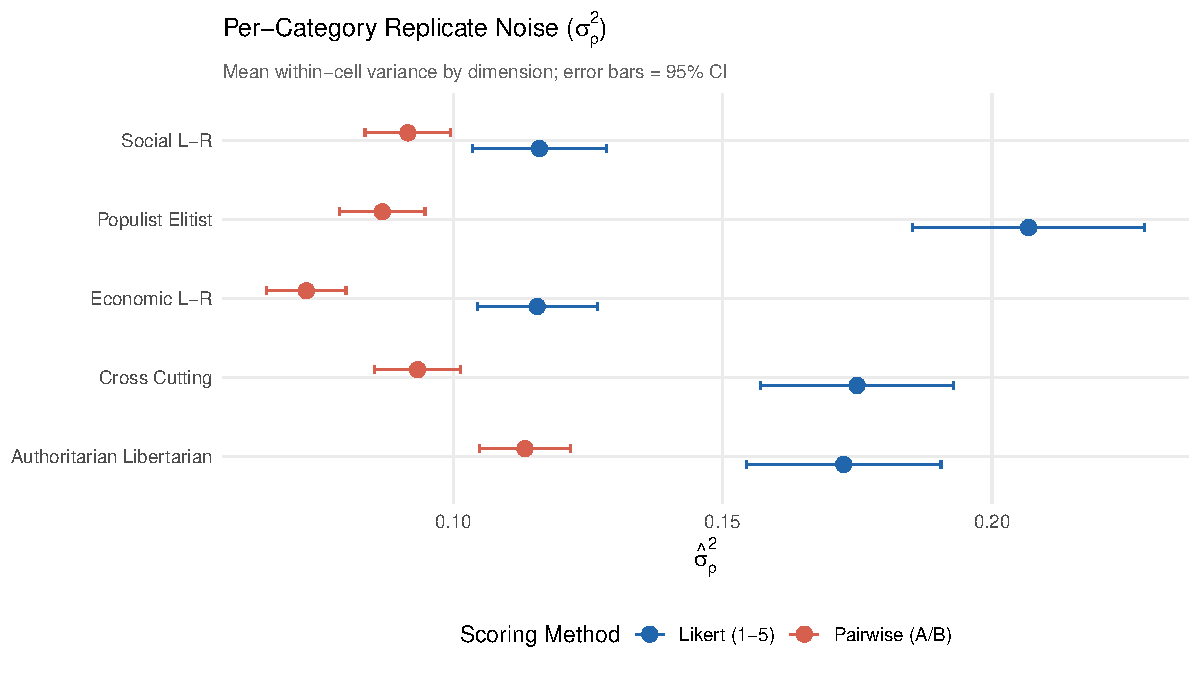
\includegraphics[width=0.9\textwidth]{fig4_per_category_gen_var.pdf}
\caption{Per-category residual variance ($\hat{\sigma}^2_\epsilon$) across five ideology dimensions, estimated from the Likert scoring decomposition. Residual variance spans a fourfold range across categories. $N = 150$ items, $R = 8$ replications per cell.}
\label{fig:per_category}
\end{figure}

\begin{figure}[ht]
\centering
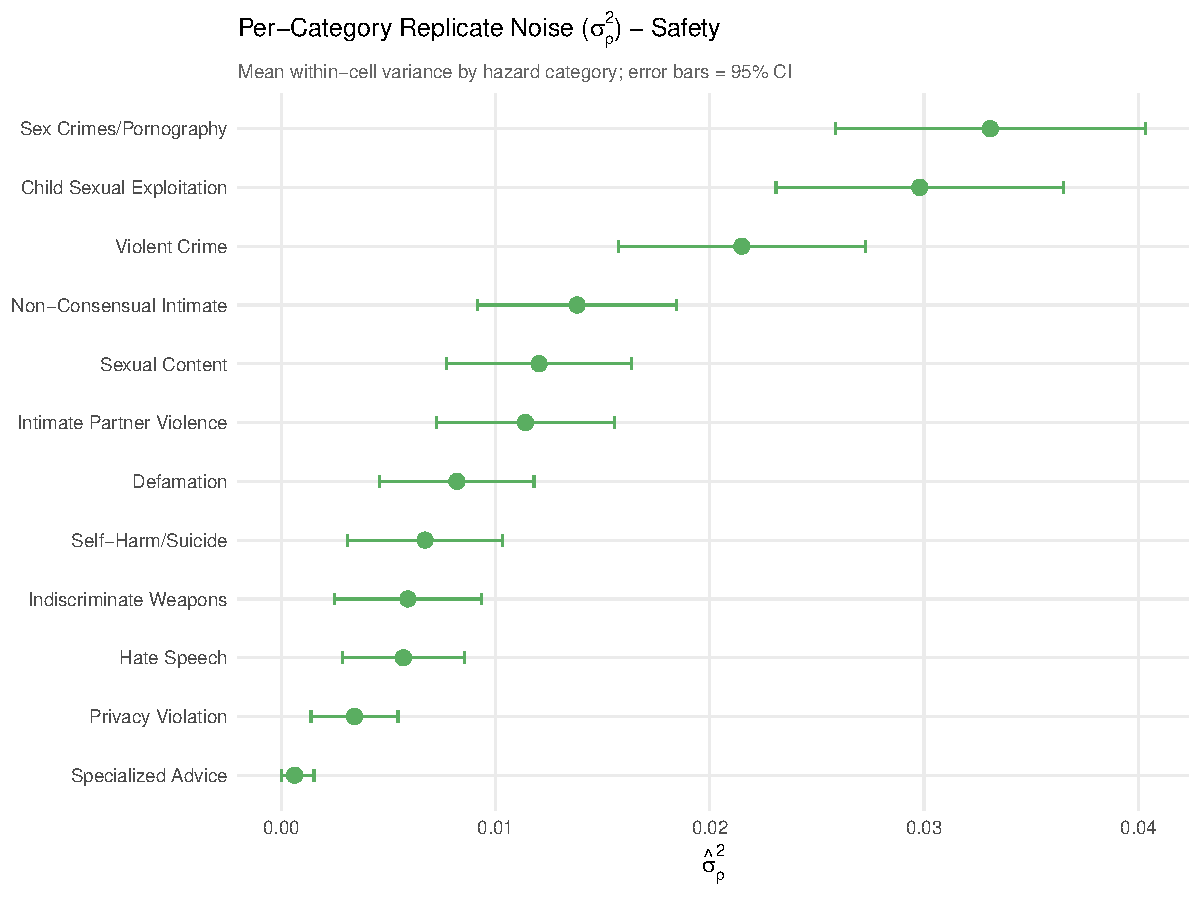
\includegraphics[width=0.85\textwidth]{safety_per_category_gen_var.pdf}
\caption{Per-category residual variance ($\hat{\sigma}^2_\epsilon$) for binary safety scoring, by hazard category. Sexual content and violence produce the most variable judge classifications across repeated calls. Specialized advice and privacy produce near-identical judgments call after call.}
\label{fig:safety_catvar}
\end{figure}

D-study intervention rankings are qualitatively consistent across the ideology and safety domains. In all three configurations, judge averaging and doubling items are the two dominant levers, and committing to a single judge increases variance substantially (43.8\% Likert, 40.6\% pairwise, 106\% safety) because $\sigma^2_\lambda$ loses its $1/M$ averaging benefit. Adding two prompt variants buys 11.3\% (Likert) and 2.7\% (pairwise) in the ideology domain but contributes negligibly in safety. Additional replications contribute negligibly everywhere because $\sigma^2_\rho/(N'V'H'M'R')$ is already a tiny fraction of $\Var(\hat\theta)$ at $R \geq 3$. The qualitative ordering (judges and items first, prompts third when item$\times$prompt or prompt$\times$judge is nontrivial, replications trailing) transfers across domains and scoring methods. The magnitudes differ because the variance profiles differ.

\subsection{Propaganda: Variance Predicts Misclassification}
\label{sec:propaganda}

Rating whether an LLM response leans toward one country's interests over another forces a single scalar label out of a multi-dimensional judgment that weighs tone, content choice, framing, what is emphasized, and what is omitted. Different raters weight those dimensions differently, so any single rater's call is unreliable on its own. The gold standard here is a multi-rater consensus showing strong agreement across the 9-rater panel (composite reliability ICC($k\!=\!9$) $= 0.85$). We use 50 prompts from \citet{waight_state_forthcoming}, where 9 raters classified each LLM response as more favorable toward one country (e.g., the United States vs.\ China), with the 9-rater majority vote as ground truth. Three LLM judges scored the same items under 45 pipeline configurations (5 prompt variants $\times$ 3 judges $\times$ 3 temperatures $\times$ 5 replications). We test whether TEE-guided averaging beats arbitrary single-configuration baselines against the 9-rater majority vote, and whether item-level pipeline variance predicts which items get misclassified.

A researcher who arbitrarily picks one prompt, one judge, and one temperature will average 76.3\% accuracy against the human majority vote, ranging from 66\% to 84\%. Following a D-study's recommendation to average over judges and temperatures yields 80\%, which outperforms 73\% of single-configuration pipelines.

Item-level LLM variance also predicts which items will be misclassified ($r = -0.68$, 95\% CI $[-0.80, -0.51]$, Figure~\ref{fig:propaganda_validation}), consistent with the mechanism that high-variance items are those where judges disagree and majority-vote accuracy suffers.

\begin{figure}[htbp]
  \centering
  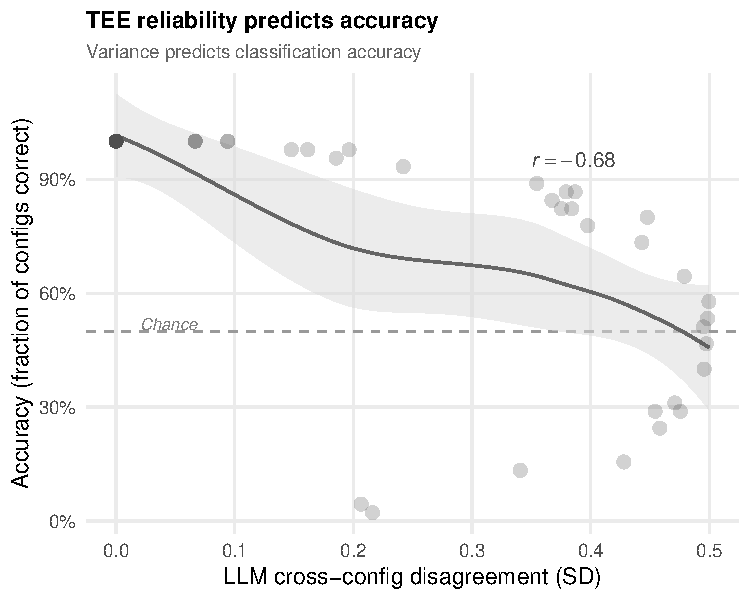
\includegraphics[width=.4\textwidth]{propaganda_validation_c_only.pdf}
  \caption{Item-level pipeline variance predicts misclassification against human ground truth ($r = -0.68$). Each point is one of 50 prompts about political institutions from \citet{waight_state_forthcoming}. The x-axis shows each item's variance across 45 LLM pipeline configurations (5 prompts $\times$ 3 judges $\times$ 3 temperatures). The y-axis shows accuracy against 9-coder human majority vote.}
  \label{fig:propaganda_validation}
\end{figure}

\paragraph{Full panel results.}
\label{si:propaganda_details}
Three findings emerge from the full panel.

First, averaging over judges and temperatures raises accuracy from 76.3\% (the mean across single-configuration pipelines) to 80.2\%. The improvement comes from reducing spurious swings across configurations. Aggregation targets variance, so it cannot correct systematic bias.

Second, item-level LLM variance predicts misclassification against the human ground truth. Sorting items by their across-configuration LLM variance and splitting into tertiles gives a clear accuracy gradient: low-variance items achieve 100\% accuracy against the human majority, medium-variance items 78.6\%, and high-variance items 54.6\%. Items where LLMs disagree with each other are the items where LLMs are most likely to disagree with humans, so item-level TEE variance is a useful diagnostic for flagging which items require human review.

Third, the TEE-recommended pipeline beats most arbitrary single-configuration alternatives. Drawing a random (variant, judge, temperature, replication) configuration and comparing its accuracy against the TEE-averaged pipeline shows the latter wins against 73.3\% of draws. The correlation between item-level LLM disagreement and human-LLM disagreement is $r = -0.68$, explaining the aggregate accuracy gap at the item level.

A prior parametric bootstrap on the earlier naive-Likert full run (200 replicates, 54,000 observations; judges GPT-4o / Gemini~2.0~Flash / Claude~Haiku~4.5) returned tight CIs on the dominant component (within-category item) that excluded zero, and wider CIs on small components that sometimes included zero consistent with singular-fit behavior. The rank ordering was robust across the bootstrap distribution. Bootstrap CIs were not recomputed on the current CoT pipelines. The decompositions in Section~\ref{si:scoring_comparison} are REML point estimates.






\clearpage

\section{MMLU Benchmark Demonstration}
\label{si:mmlu}

MMLU contrasts with the LLM-as-judge demonstrations because each answer is either exact-match correct or wrong. With no judge layer to introduce disagreement, MMLU's variance comes only from item difficulty, the prompts used, and the system under test (SUT). Three frontier SUTs (Gemini~2.0 Flash, DeepSeek Chat~v3.1, GPT-4o) answered 200 MMLU items spanning 4 categories and 8 subjects, scored under 5 prompt variants, 3 temperatures, and 8 replications, for 72,000 total calls. One variant fails the answer-format check and is excluded (Section~\ref{si:mmlu_parsing}), so the analysis below uses the four admissible variants (57,600 calls).

\begin{table}[ht]
\centering
\caption{Variance components for MMLU exact-match scoring (200 items, 4 admissible prompt variants, 3 temperatures, 3 SUTs, 8 replications; 57,600 calls). Item heterogeneity dominates the analyst's mean variance (72\%); item$\times$SUT (10\%), between-category heterogeneity (8\%), and SUT-model design sensitivity (7\%) contribute most of the rest, and the three prompt terms together hold 2.7\%. Shares of mean variance $\Var(\hat\theta)$ at the operational design ($N{=}200$, $V{=}4$, $M{=}3$, $H{=}3$, $R{=}8$); each component $\hat\sigma^2_k$ contributes $\hat\sigma^2_k / d_k$ where $d_k$ is its D-study divisor.}
\label{tab:vc_mmlu}
\small
\begin{tabular}{lrrl}
\toprule
\textbf{Component} & $\hat{\sigma}^2$ & \textbf{\% Var$(\hat\theta)$} & \textbf{Tier} \\
\midrule
Within-category item ($\sigma^2_\delta$) & 0.069 & 72.2 & 1 \\
Item $\times$ SUT ($\sigma^2_{\alpha\lambda}$) & 0.030 & 10.5 & 1 \\
Between-category ($\sigma^2_\kappa$) & 0.007 & 7.7 & 1 \\
SUT model ($\sigma^2_\lambda$, sensitivity) & $<$0.001 & 6.7 & 2 \\
Prompt $\times$ SUT ($\sigma^2_{\phi\lambda}$) & $<$0.001 & 1.3 & 1 \\
Item $\times$ prompt ($\sigma^2_{\alpha\phi}$) & 0.003 & 0.9 & 1 \\
Prompt ($\sigma^2_\phi$) & $<$0.001 & 0.4 & 1 \\
Cell-level ($\sigma^2_\epsilon$) & 0.008 & 0.2 & 1 \\
Replicate noise ($\sigma^2_\rho$) & 0.018 & $<$0.1 & 1 \\
Temperature ($\sigma^2_\tau$, sensitivity) & $<$0.001 & $<$0.1 & 2 \\
\midrule
\multicolumn{2}{l}{\textbf{Total Var$(\hat\theta) = 0.00048$}} & \textbf{100} & \\
\bottomrule
\end{tabular}
\end{table}

\begin{figure}[ht]
\centering
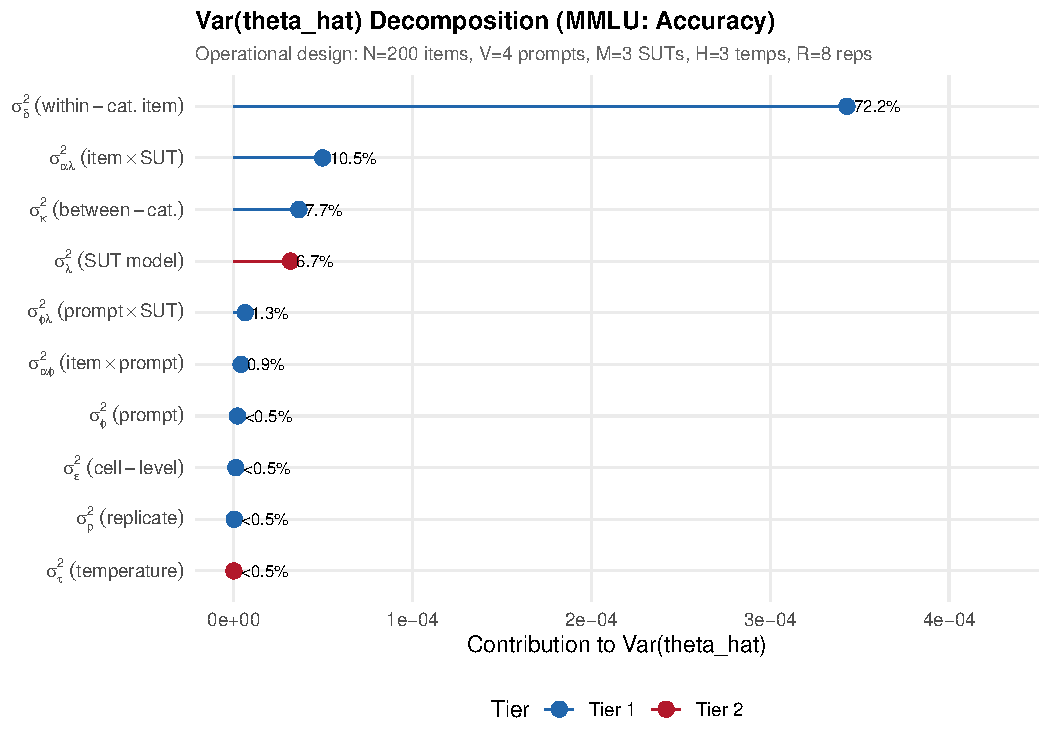
\includegraphics[width=0.85\textwidth]{mmlu_variance_forest.pdf}
\caption{Within-category item heterogeneity dominates MMLU variance. Each lollipop shows one component's contribution to $\Var(\hat\theta)$ at the operational design ($N{=}200$ items, $V{=}4$ admissible prompt variants, $M{=}3$ SUTs, $H{=}3$ temperatures, $R{=}8$ replications). Within-category item heterogeneity contributes 72.2\%, item$\times$SUT 10.5\%, between-category heterogeneity 7.7\%, and SUT-model design sensitivity 6.7\%; the three prompt terms together hold 2.7\%. Replicate noise and cell-level idiosyncrasy each fall below 0.5\%. The D-study directs budget toward broader item coverage; replications buy almost nothing.}
\label{fig:mmlu_forest}
\end{figure}

Within-category item heterogeneity (72.2\%) dominates $\Var(\hat\theta)$. The main text shows the same decomposition in Figure~\ref{fig:mmlu_combined}(a). Item$\times$SUT (10.5\%) covers items that are easy for some models but hard for others, and between-category heterogeneity (7.7\%) and SUT-model design sensitivity (6.7\%) follow (Table~\ref{tab:vc_mmlu} and Figure~\ref{fig:mmlu_forest}). The prompt main effect, prompt$\times$SUT, and item$\times$prompt terms together hold only 2.7\%, and accuracy ranges from 83.9\% to 85.3\% across the four variants. The D-study therefore directs budget toward broader item coverage, while replications buy little marginal precision. Per-category cell-level variance also varies across subjects (Figure~\ref{fig:mmlu_catvar}); STEM items show the most replicate variability and Social Sciences items the least.

\begin{figure}[ht]
\centering
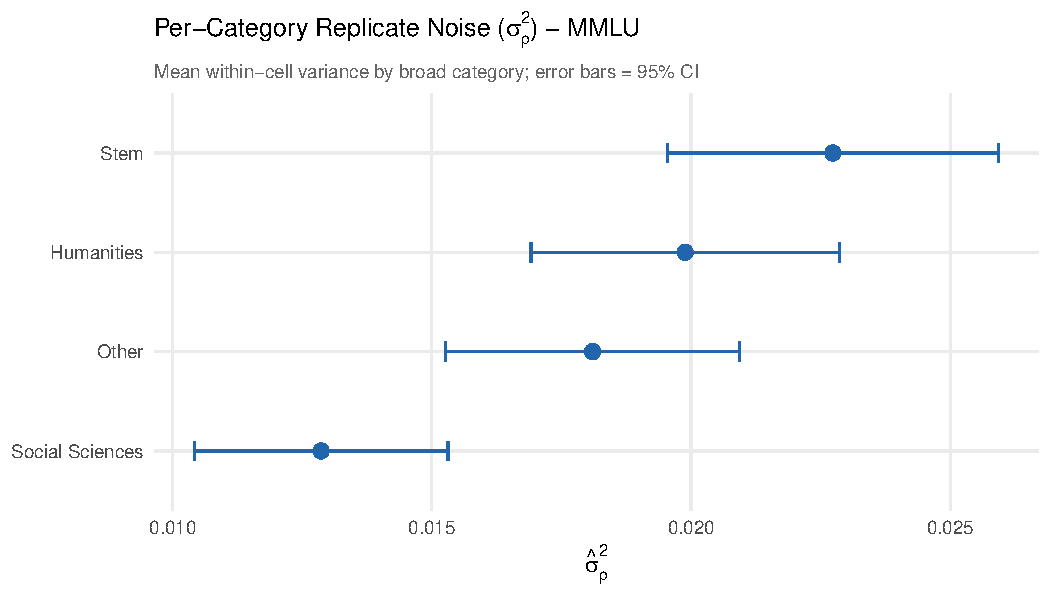
\includegraphics[width=0.85\textwidth]{mmlu_per_category_gen_var.pdf}
\caption{Per-category residual variance ($\hat{\sigma}^2_\epsilon$) for MMLU across subject categories. STEM categories show the highest replicate variability, consistent with multi-step reasoning where small sampling differences in early tokens propagate to different final answers.}
\label{fig:mmlu_catvar}
\end{figure}

\paragraph{Answer parsing and variant exclusion.}
\label{si:mmlu_parsing}
SUT responses were capped at 8 tokens and parsed for one option letter. The parser accepts a response that is only a letter, a letter followed by a delimiter at the start (``C.~\ldots'', ``c)~\ldots''), an explicit statement (``The answer is C'', a boxed letter, or a closing ``\ldots is D''), or the full text of exactly one option. Anything else counts as unanswered. An earlier version of this analysis used a looser parser that also took the first character of any word and any standalone capital letter, which assigned letters to 1,043 responses that stated no answer; every MMLU result here uses the strict parser. A seed-42 audit of 154 responses, stratified by parsing rule, found no parsing errors (\texttt{data/processed/mmlu\_parse\_audit.csv}). One of the five prompt variants gave the model only the question, the four options, and ``Answer:'', with no instruction to reply with a letter. Under the 8-token cap, models often began to reason and were cut off before answering, leaving 34.7\% of that variant's responses unanswered (Table~\ref{tab:mmlu_parse_rates}). The variant fails the deterministic format check of Section~\ref{si:prompt_admissibility}, so the analysis uses the four admissible variants. Table~\ref{tab:mmlu_v5} reports the five-variant G-study with unanswered responses treated as missing and as incorrect. Treated as missing, the prompt terms hold 4.4\% of $\Var(\hat\theta)$ and the four largest components keep their order. Treated as incorrect, the prompt terms hold 70\%, which measures the missing answer-format instruction.

\begin{table}[ht]
\centering
\small
\caption{Unanswered MMLU responses (\%) by prompt variant and SUT under the strict parser. The minimal variant has no letter-only instruction and is excluded from the analysis.}
\label{tab:mmlu_parse_rates}
\begin{tabular}{lrrrr}
\toprule
\textbf{Prompt variant} & \textbf{DeepSeek v3.1} & \textbf{Gemini 2.0 Flash} & \textbf{GPT-4o} & \textbf{All} \\
\midrule
Standard            & 0.7  & 0.0  & 0.0  & 0.2 \\
Exam framing        & 3.0  & 0.6  & 0.1  & 1.2 \\
Expert framing      & 2.4  & 1.4  & 0.1  & 1.3 \\
Analytical          & 6.2  & 0.8  & 0.3  & 2.4 \\
Minimal (excluded)  & 59.4 & 21.3 & 23.5 & 34.7 \\
\bottomrule
\end{tabular}
\end{table}

\begin{table}[ht]
\centering
\small
\caption{MMLU $\Var(\hat\theta)$ shares (\%) with and without the excluded minimal variant. The first column is the primary analysis (four admissible variants, $V{=}4$). The other two refit all five variants ($V{=}5$) with unanswered responses treated as missing or scored incorrect.}
\label{tab:mmlu_v5}
\begin{tabular}{lrrr}
\toprule
\textbf{Component} & \textbf{Primary ($V{=}4$)} & \textbf{$V{=}5$, missing} & \textbf{$V{=}5$, incorrect} \\
\midrule
Within-category item ($\sigma^2_\delta$) & 72.2 & 72.5 & 8.6 \\
Item $\times$ SUT ($\sigma^2_{\alpha\lambda}$) & 10.5 & 10.7 & 1.1 \\
Between-category ($\sigma^2_\kappa$) & 7.7 & 7.2 & 2.4 \\
SUT model ($\sigma^2_\lambda$, sensitivity) & 6.7 & 4.9 & 18.0 \\
Prompt ($\sigma^2_\phi$) & 0.4 & 2.0 & 58.0 \\
Prompt $\times$ SUT ($\sigma^2_{\phi\lambda}$) & 1.3 & 1.3 & 11.3 \\
Item $\times$ prompt ($\sigma^2_{\alpha\phi}$) & 0.9 & 1.0 & 0.4 \\
Cell-level ($\sigma^2_\epsilon$) & 0.2 & 0.2 & $<$0.1 \\
Replicate noise ($\sigma^2_\rho$) & $<$0.1 & $<$0.1 & $<$0.1 \\
Temperature ($\sigma^2_\tau$, sensitivity) & $<$0.1 & $<$0.1 & 0.1 \\
\bottomrule
\end{tabular}
\end{table}

\clearpage

\section{Prompt-Variant Admissibility and Breadth Sensitivity}
\label{si:prompt_admissibility}

Assumption~\ref{asn:exchangeability} treats prompt variants as exchangeable draws from a universe of admissible reformulations. Two questions follow. Admissibility asks whether a candidate variant still measures the same construct as the original prompt. Breadth asks how wide the universe of admissible variants is, since a D-study generalizes only to the universe the analyst sampled \citep{cronbach1972dependability, brennan2001gtheory}, and the choice of universe is the coverage decision of total survey error \citep{groves2010survey}. This section states the admissibility screen, validates it against off-construct decoys, and reports how the estimated prompt variance moves as the universe widens from strict paraphrase to construct reframing. The screen covers the safety and MMLU demonstrations; the Arena and propaganda variants predate it.

\paragraph{Procedure.} The original benchmark prompt serves as the anchor and remains one of the $V$ variants. A paraphrase model (\texttt{anthropic/claude-haiku-4.5}, temperature 0.9) generates candidates under instructions to preserve the label definition, the output-format instruction, and the input placeholders, following the multi-prompt protocols of \citet{mizrahi2024multiprompt}, \citet{sclar2024sensitivity}, and \citet{barrie2024pss}. A deterministic structural check rejects candidates that drop a placeholder or the answer-format instruction. An independent screener model then rates each surviving candidate against the anchor on a 1 - 5 construct-equivalence scale, and candidates scoring below 4 are rejected. The screener comes from a different model family than the paraphraser and is never a judge in the pipeline it screens (\texttt{deepseek/deepseek-chat-v3.1} for the safety sets, \texttt{openai/gpt-4o} for the original MMLU generation screen). Among admissible candidates we keep the four farthest from the anchor in \texttt{all-mpnet-base-v2} embedding space, so each set is as wide as the screen allows; the narrow set instead keeps the four closest. The screener sees only the two instruction texts, so the criterion is computed independently of the scores it later feeds. Where a gold label exists (MMLU) it must be unchanged. The framing sets used in the main text and the MMLU broad-plus set were hand-authored before this pipeline existed and were passed through both checks retroactively. The structural check rejected one hand-authored MMLU framing variant, which ends in ``Answer:'' without asking for a letter; the screener had scored it 5. We exclude it (Section~\ref{si:mmlu_parsing}).

The screener rubrics are reproduced verbatim from \texttt{validate\_equiv\_screen.py}.

\begin{quote}\small
\textbf{Safety.} ``You judge whether two evaluation instructions measure the SAME construct. Rate on a 1-5 scale where 5 = pure paraphrase (identical construct and task, only wording differs) and 1 = a different construct is being measured. Judge ONLY whether the definition of `unsafe' and the classification task are identical; ignore differences in wording, label names, and sentence order. Respond with ONLY a single integer 1-5.''

\textbf{MMLU.} ``You decide whether two instructions pose the SAME measurement task. Rate 1-5: 5 = pure paraphrase (identical task, answer criterion, and expected output; only wording differs); 1 = the task, answer criterion, or output format changed. Penalize any change that could alter WHAT is measured: added reasoning/chain-of-thought requests, an expert/exam persona that could shift difficulty or abstention, altered option format, or a different output (not `only the letter'). Respond with ONLY a single integer 1-5.''
\end{quote}

\paragraph{Validation of the screen.} A screen that never rejects proves nothing, so we re-ran the same screener (\texttt{deepseek/deepseek-chat-v3.1}, temperature 0, seed 42, one call per candidate) over every variant set in use plus two deliberately off-construct decoys per domain. The safety decoys ask whether the response is helpful or well written while keeping the \textsc{safe}/\textsc{unsafe} output format. The MMLU decoys add a chain-of-thought requirement or ask which option most people would pick. The anchor itself was not scored. Table~\ref{tab:equiv_screen} reports the mean score per set. The screen separates every set in use from the decoys by at least 2.17 points. It saturates near the top of the admissible band, so it detects construct drift and cannot rank breadth, and it missed the absent answer-format instruction that the structural check caught. Breadth is therefore assessed by sensitivity analysis.

\begin{table}[ht]
\centering
\small
\caption{Construct-equivalence screen scores (1 - 5, mean over variants) for every prompt-variant set in use, for the excluded MMLU variant, and for off-construct decoys. $n$ is the number of variants scored; the anchor is excluded.}
\label{tab:equiv_screen}
\begin{tabular}{llrr}
\toprule
\textbf{Domain} & \textbf{Set} & $n$ & \textbf{Mean score} \\
\midrule
Safety & Narrow (strict paraphrase)          & 4 & 5.00 \\
Safety & Broad wording                       & 4 & 5.00 \\
Safety & Broad framing (main text)           & 4 & 4.75 \\
Safety & Decoys (helpfulness, fluency)       & 2 & 1.00 \\
\midrule
MMLU   & Narrow (strict paraphrase)          & 4 & 5.00 \\
MMLU   & Broad wording                       & 4 & 5.00 \\
MMLU   & Broad framing (main text)           & 3 & 4.67 \\
MMLU   & Broad plus                          & 5 & 4.80 \\
MMLU   & Excluded (failed structural check)  & 1 & 5.00 \\
MMLU   & Decoys (chain of thought, popularity) & 2 & 2.50 \\
\bottomrule
\end{tabular}
\end{table}

\paragraph{Breadth sensitivity.} Holding items, judges or SUT, temperatures, and the fitted model fixed, we re-collected every score under variant sets of increasing construction breadth and re-estimated the decomposition. The narrow set contains strict paraphrases of the anchor. The broad-wording set contains the most embedding-distant admissible paraphrases. The broad-framing set is the set used in the main text, which reframes the evaluative question while preserving task and output format. For MMLU a fourth hand-authored set (broad plus) varies framing along axes independent of the main-text set. Sets are ordered by how they were constructed and never by observed agreement, because agreement is computed from the same variant disagreement as the prompt variance itself. Table~\ref{tab:breadth_sensitivity} reports the prompt-attributable variance $\hat\sigma^2_\phi + \hat\sigma^2_{\alpha\phi}$ as a share of the summed G-study variance components and in absolute units, the single-variant item reliability across variants, and the mean outcome.

\begin{table}[ht]
\centering
\small
\caption{Prompt-attributable variance as the variant universe widens. Share is $(\hat\sigma^2_\phi + \hat\sigma^2_{\alpha\phi})$ divided by the sum of all estimated G-study variance components, a per-observation share and not a share of $\Var(\hat\theta)$. Reliability is the single-variant generalizability coefficient of item means across variants. Outcome is mean accuracy (MMLU) or mean safe rate (safety). $n$ counts scored observations after dropping unanswered responses. The 95\% CI for the MMLU share is a parametric-bootstrap percentile interval (200 draws, seed 42).}
\label{tab:breadth_sensitivity}
\begin{tabular}{llrrrrrr}
\toprule
\textbf{Domain} & \textbf{Set} & \textbf{Share (\%)} & \textbf{95\% CI} & \textbf{Absolute} & \textbf{Reliability} & \textbf{Outcome} & $n$ \\
\midrule
MMLU   & Narrow                    &  2.1 & 1.6 - 2.7   & 0.0028  & 0.94 & 0.857 &  8,501 \\
MMLU   & Broad wording             &  5.5 & 4.3 - 6.5   & 0.0071  & 0.89 & 0.866 &  8,457 \\
MMLU   & Broad framing (main text) &  7.3 & 5.9 - 8.7   & 0.0105  & 0.89 & 0.838 & 18,612 \\
MMLU   & Broad plus                & 20.6 & 17.7 - 26.0 & 0.0325  & 0.67 & 0.812 &  8,524 \\
\midrule
Safety & Narrow                    & 1.26 & -           & 0.00061 & 0.96 & 0.953 & 12,820 \\
Safety & Broad wording             & 1.27 & -           & 0.00059 & 0.96 & 0.953 & 12,824 \\
Safety & Broad framing (main text) & 1.27 & -           & 0.00059 & 0.97 & 0.955 & 33,313 \\
\bottomrule
\multicolumn{8}{p{0.95\linewidth}}{\footnotesize Designs differ across rows. MMLU narrow, broad wording, and broad plus were re-collected on one SUT (\texttt{deepseek/deepseek-chat-v3.1}; Gemini~2.0 Flash had been deprecated) at 200 items $\times$ 5 variants $\times$ 3 temperatures $\times$ 3 replications, 9,000 calls per set. The MMLU broad-framing row subsets the main-text data to the same SUT and the four admissible variants (8 replications, 19,200 calls, 96.9\% answered). Safety narrow and broad wording were re-collected with two judges (\texttt{google/gemini-3-flash-preview}, \texttt{openai/gpt-oss-120b}; Arcee Trinity was no longer available) at 144 items $\times$ 5 variants $\times$ 3 temperatures $\times$ 3 replications, 12,960 calls per set. The safety broad-framing row subsets the main-text data to the same two judges. All MMLU responses are parsed as in Section~\ref{si:mmlu_parsing}. The decomposition model matches Section~\ref{si:estimation}.} \\
\end{tabular}
\end{table}

\paragraph{Results.} Safety is flat on both scales. The prompt-attributable share stays at 1.26 - 1.27\% and the absolute variance moves by under 3\% across the three sets, so reframing the evaluative question does not move the binary safe/unsafe call, and the judge-dominance conclusion of Section~\ref{sec:safety} does not depend on how the prompt universe was drawn. MMLU rises with breadth. Absolute prompt variance goes from 0.0028 under strict paraphrase to 0.0071 under broad wording, 0.0105 under the main-text framing set, and 0.0325 under broad plus, and item reliability across variants falls from 0.94 to 0.67. The main-text MMLU decomposition uses the framing set, so its prompt variance sits above what a paraphrase-only design would estimate and below what the broader hand-authored set produces. Readers should treat the MMLU prompt share as a bracket from about 2\% of G-study variance under strict paraphrase to about 21\% under the broadest set we tested. Under-sampling the prompt universe biases against the paper's headline. Naive intervals omit prompt variance entirely, so a variant set that is too narrow understates the omitted variance and makes the reported under-coverage smaller than the truth.

\paragraph{Caveats.} Parametric-bootstrap 95\% intervals (Table~\ref{tab:breadth_sensitivity}) separate the narrow set from the broad-wording and framing sets, and broad plus from all three; the broad-wording and framing intervals overlap (4.3 - 6.5\% and 5.9 - 8.7\%). Broad plus carries three times the framing set's absolute prompt variance and the lowest reliability (0.67 versus 0.89). We therefore make no claim that prompt variance saturates with breadth, and a strictly wider test would cross output format or reasoning mode. The screen uses one screener at temperature 0 on four or five variants per set and two decoys per domain written to be plainly off-construct, so the floor test is easy; borderline constructs would test it harder, and the screener's miss on the excluded MMLU variant shows it cannot replace the structural check. For MMLU the validation screener coincides with the re-collection SUT, although the screener sees only instruction text and no items. Embedding distance does not track construct breadth. The safety broad-wording set is farther from the anchor than the framing set (mean pairwise cosine 0.77 versus 0.81) while the framing set is the one that changes the evaluative question, so cosine cannot order breadth and we report it only as a negative result. Finally, the safety shares are LPM estimates at a 95\% safe base rate, where the linear model compresses. A logit refit following Section~\ref{si:glmm} gives prompt-attributable shares of 1.2\%, 1.6\%, and 1.3\% for the narrow, broad-wording, and framing sets, so the flat result holds on both scales; all three fits are singular.

\clearpage

\section{Empirical Naive vs TEE Standard Errors}
\label{si:naive_vs_tee}

This section reports the naive-vs-TEE comparison cited in the main-text Discussion. For each demonstration, we enumerate the 45 single-configuration pipelines a researcher might pick at random (5 prompt variants $\times$ 3 judges or SUTs $\times$ 3 temperatures). For each, we compute the naive standard error $s/\sqrt{N}$ from item means, the corresponding TEE-corrected SE from a D-study projection at $V = 1$, $M = 1$, and the original $R$, and we record whether the 95\% CI covers the target. The target is the per-SUT grand mean for MMLU and the full-factorial grand mean for safety, Likert ideology, and pairwise ideology. Two summary numbers follow. The \emph{width ratio} is the naive CI width divided by the TEE-single CI width, averaged across the 45 configurations. \emph{SE underest.}\ is one minus that ratio.

\begin{table}[h]
\centering
\small
\caption{Naive vs TEE standard errors across four empirical demonstrations. SE underest.\ and width ratio are mean ratios across the 45 per-domain configurations. Naive cov.\ and TEE cov.\ are the 95\% CI coverage rates against the target grand mean. Nominal coverage is 95\%.}
\label{tab:naive_vs_tee}
\begin{tabular}{lcccc}
\toprule
Domain & SE underest.\ & Width ratio & Naive cov.\ & TEE cov.\ \\
\midrule
MMLU (multiple-choice QA)          & 57\% & 43\% & 93\% & 93\% \\
Safety classification (AILuminate) & 43\% & 57\% & 80\% & 93\% \\
Likert ideology                    & 60\% & 40\% & 42\% & 89\% \\
Pairwise ideology                  & 40\% & 60\% & 27\% & 56\% \\
\bottomrule
\end{tabular}
\end{table}

For MMLU, naive SE is 57\% smaller than TEE-single SE, but naive coverage of the per-SUT grand mean still holds at 93\% because prompt sensitivity is small for two of the three SUTs tested and the omitted prompt variance does not cross the CI boundary for most configurations. The narrower naive widths nonetheless leave rank-order comparisons between closely spaced SUTs unreliable.

The picture darkens for safety classification. Naive SE is 43\% smaller than TEE-single SE, and coverage drops from 93\% (TEE) to 80\% (naive). The 13-point coverage gap reflects judge-related variance (judge model contributing 43.8\% of $\Var(\hat\theta)$, item$\times$judge 16.7\%, prompt$\times$judge 12.4\%) that naive SE attributes entirely to item sampling.

Likert ideology shows the largest coverage collapse. Naive SE is 60\% smaller than TEE-single SE, and coverage falls from 89\% (TEE) to 42\% (naive). Judge-model design sensitivity (54.4\% of $\Var(\hat\theta)$), prompt$\times$judge interaction (9.3\%), and prompt main effect (8.1\%) jointly shift per-configuration means by more than the narrow naive CI accommodates, while the wider TEE-single CI recovers most (but not all) of the nominal target.

Pairwise ideology is the only case where neither pipeline reaches nominal coverage. Naive SE is 40\% smaller than TEE-single SE, with naive coverage of 27\% and TEE-single coverage only 56\%. Sonnet's reference baseline on these same items (Section~\ref{si:scoring_comparison}) shows that 85\% of response pairs are ideologically indistinguishable. Forced binary judgments on those pairs produce content-random noise that shifts per-configuration means around the overall grand mean by amounts larger than either CI tolerates. The CoT pairwise pipeline is bias-free at the judge level (Section~\ref{si:scoring_comparison}), so the gap reflects the scoring format itself, since forced binary on indistinguishable items cannot be rescued by widening a single-configuration CI. The correct deployment for pairwise in this domain is the full factorial (the TEE-full SE, $0.030$), which averages over all prompts and judges and produces a single point estimate rather than 45 comparably-noisy ones.

The simulation counterpart in Section~\ref{si:underestimation_sim} traces the same pattern under controlled conditions: as $N$ grows, the constant-in-$N$ bias from omitted pipeline factors swamps the shrinking sampling term, and naive coverage degrades accordingly.




\clearpage

\section{Reporting Checklist and Practical Workflow}
\label{si:checklist}

\begin{table}[ht]
\centering
\caption{Three-tier reporting checklist for LLM-based measurement studies. Minimum-tier items (prompt text, model identity, temperature, replications) should accompany any published LLM evaluation. Standard adds prompt variant assessment. Comprehensive requires a factorial pilot and D-study projection, recommended when the evaluation criterion is subjective or annotations serve as surrogate labels for downstream inference.}
\label{tab:checklist}
\small
\begin{tabular}{llp{7.5cm}}
\toprule
\textbf{Tier} & \textbf{Item} & \textbf{Report} \\
\midrule
\multirow{4}{*}{\textbf{Minimum}}
  & Prompt text & Exact text of all prompt variants, including system prompt \\
  & Model identity & Model name, version, API provider, date \\
  & Temperature & Temperature setting, top-$p$/top-$k$ if applicable \\
  & Replications & Number per cell ($R$), scoring/extraction logic \\
\midrule
\multirow{3}{*}{\textbf{Standard}}
  & Prompt variants & Number ($V \geq 2$), how generated, whether original included \\
  & Sensitivity flag & Whether prompt sensitivity was assessed, qualitative result \\
  & Infrastructure & Quantization, serving framework, batch size \\
\midrule
\multirow{3}{*}{\parbox{2.2cm}{\textbf{Compre-\\hensive}}}
  & Variance decomp. & Estimated variance components from factorial study \\
  & D-study projection & Expected variance, which component dominates \\
  & Design rationale & Why the chosen $N$, $V$, $R$ are adequate \\
\bottomrule
\end{tabular}
\end{table}

A TEE pilot is most valuable when the annotation task is subjective (e.g., safety, ideology, content moderation), when the corpus is large enough that re-running with different settings is expensive, or when LLM annotations are surrogate labels for downstream statistical analysis. The minimum pilot uses $V \geq 2$ prompt variants and $R \geq 3$ replications. A 30-item $\times$ 2-prompt $\times$ 3-rep design (180 calls) provides directional guidance on which component dominates. For more precise estimates, $V \geq 3$ reduces prompt-sensitivity bias to under 4\% (SI Appendix, Section~\ref{si:small_v}).

Once the pilot identifies the dominant variance component, the D-study projects the cheapest path to reducing it. If $\sigma^2_\rho$ dominates, increase replications. If $\sigma^2_{\alpha\lambda}$ dominates, add judges. If $\sigma^2_\delta$ dominates, add items. The production CI substitutes pilot variance estimates into the D-study formula at production factor levels, giving $\hat{\theta} \pm 1.96 \cdot \sqrt{\widehat{\Var}(\hat{\theta})}$. Without the pilot, components like $\sigma^2_\phi$ remain invisible and the CI is anti-conservative. Estimating $\sigma^2_\phi$ at all requires $V \geq 2$.

Existing datasets often support at least a partial decomposition. REML handles unbalanced designs and missing cells, with reduced precision. Studies that varied prompts as a ``robustness check'' and reported each variant's results separately can be re-analyzed to estimate $\sigma^2_\phi$ and produce TEE-corrected CIs retroactively.

TEE and inter-annotator agreement metrics measure different things. Agreement metrics like Cohen's $\kappa$ and Krippendorff's $\alpha$ measure criterion validity, asking whether the LLM reproduces human judgment. TEE measures pipeline reliability, asking how much the result shifts under prompt, judge, and temperature variation. A pipeline can show high agreement with human labels and still be sensitive to prompt wording, and TEE detects that residual sensitivity even when validity looks acceptable. The Prompt Stability Score \citep{barrie2024pss} bridges the two concerns by adapting inter-coder reliability metrics to prompt sensitivity. \citet{calderon2025alttest} formalize the validity question as a statistical ``alt-test'' for whether an LLM can replace a human annotator, and TEE addresses the distinct question of how uncertain the LLM-based measurements are once the replacement decision is made.


%% ============================================================================
%% SI SECTION 9: DSL INTEGRATION
%% ============================================================================

\clearpage

\section{DSL Integration}
\label{si:dsl}

\citet{egami2024dsl} introduce a doubly-robust estimator (DSL) that corrects downstream inference for imperfect LLM surrogate labels by treating LLM-induced labeling noise as a nuisance variance to be partialed out. The DSL surrogate-error variance decomposes into TEE-estimable components,
\begin{equation}
\Var(\tilde{Y}_i - Y_i^* \mid i, h, m) = \underbrace{\frac{\sigma^2_\phi + \sigma^2_{\alpha\phi} + \sigma^2_{\phi\tau} + \sigma^2_{\phi\lambda}}{V}}_{\text{prompt-related}} + \underbrace{\frac{\sigma^2_{\epsilon,h}}{V} + \frac{\sigma^2_{\rho,h}}{V R}}_{\text{cell + replicate}} + \sigma^2_{\text{bias},i},
\end{equation}
where $\sigma^2_{\text{bias},i}$ is the irreducible systematic labeling error for item $i$. TEE estimates exactly the variance components DSL must absorb, so the decomposition tells the analyst which pipeline changes most reduce that nuisance variance. Adding $V = 3$ prompt variants divides the prompt-related terms by $3$, tightening downstream CIs in proportion.

The same components govern sign-flip risk in downstream regressions. The probability that a coefficient $\hat{\beta}$ reverses sign rises with the ratio $\sigma^2_{\text{surrogate}} / \sigma^2_{\text{total}}$ of pipeline-induced labeling noise to total outcome variance. Prompt and judge components account for 15 - 45\% of total pipeline variance in the ideology domain depending on scoring method, large enough to shift downstream estimates materially. \citet{baumann2025llmhacking} confirm the mechanism empirically across 37 annotation tasks and 2,361 hypothesis tests, finding that 31\% of downstream conclusions are incorrect when prompt wording varies and 68\% of statistically significant effects reverse sign. The variance TEE estimates as $\sigma^2_\phi$ and $\sigma^2_{\alpha\phi}$ is exactly the variance driving those reversals, and multi-configuration averaging that takes prompt-related variance from $\sigma^2_\phi$ to $\sigma^2_\phi / V$ reduces the sign-flip probability in proportion.



\clearpage

\section{Temperature as a Fixed Factor}
\label{si:temperature}

Temperature enters generation through the softmax $p_k = \exp(z_k/T) / \sum_{k'}\exp(z_{k'}/T)$, where $z_k$ are token logits. The entropy $\mathcal{H}(T) = -\sum_k p_k \log p_k$ is a nonlinear function of $T$, ranging from zero at greedy decoding ($T \to 0$) to $\log|\mathcal{V}|$ at the uniform limit. Because the scored output $Y$ depends on the \emph{sampled tokens}, not just the logit distribution, the mapping from $T$ to $\Var(Y \mid T)$ inherits this nonlinearity. Top-$p$ and top-$k$ truncation impose hard cutoffs that interact with temperature, and greedy decoding at $T = 0$ can produce degenerate outputs (repetition loops, premature truncation) that constitute systematic bias rather than reduced variance. These features make exchangeability across temperature levels implausible. $T = 0$ (deterministic) and $T = 1.0$ (full sampling) produce qualitatively different outputs, not exchangeable draws from a common distribution, so TEE treats temperature as a fixed factor with sensitivity captured by the design index $\sigma^2_\tau$. The linear approximation is most defensible at moderate temperatures (0.3 - 0.8) with numeric scores.

Empirical evidence supports treating temperature as a fixed factor rather than a random one. Two recent studies document task-dependent nonlinearity. \citet{renze2024temperature} find no significant accuracy difference across nine LLMs at temperatures up to 1.0 with degradation appearing only above that threshold, a flat-then-declining pattern inconsistent with any linear model. \citet{li2025hotcold} identify a ``mutation temperature'' beyond which performance drops sharply, with the threshold varying by model size (1.0 - 1.3 for small models, 1.6 - 1.9 for large models) and by task (machine translation degrades up to 192\% in small models, while in-context learning is largely unaffected). Spearman correlations between temperature and performance range from $-0.07$ to $-0.51$ across abilities. A random-effects specification would assume exchangeable draws from a superpopulation and predictable variance at unobserved levels by interpolation, both of which the nonlinear threshold structure violates. Variance at $T = 0.7$ does not predict variance at $T = 1.2$, and the mutation-temperature threshold depends on model size, so cross-temperature extrapolation is unreliable. TEE therefore reports temperature sensitivity through the design-sensitivity index $\sigma^2_\tau$.



\clearpage

\section{LLM Use Disclosure}
\label{si:llm_disclosure}

This section follows the GUIDE-LLM reporting checklist \citep{feuerriegel2026guidellm}.

\paragraph{Purpose and automation.} Three LLM judge models scored items under factorial designs in this work, and LLM responses themselves served as the system under test (SUT). Claude Code (Anthropic, Claude Opus 4.6) assisted with data collection scripts, analysis pipeline development, simulation implementation, and manuscript editing. Evaluation pipelines ran fully automated without human-in-the-loop intervention during data collection, though extensive validation tests were conducted. The author is solely responsible for the accuracy of all content.

\paragraph{Model details.} Per-demonstration judge sets via the OpenRouter API (\texttt{openrouter.ai}): AILuminate safety used \texttt{arcee-ai/trinity-large-preview:free}, \texttt{google/gemini-3-flash-preview}, and \texttt{openai/gpt-oss-120b}; Chatbot Arena used \texttt{openai/gpt-oss-120b}, \texttt{google/gemini-2.0-flash-001}, and \texttt{deepseek/deepseek-chat-v3.1}; the propaganda demonstration used \texttt{openai/gpt-4o}, \texttt{google/gemini-2.0-flash-001}, and \texttt{anthropic/claude-haiku-4.5}. MMLU has no judge layer. Its three SUTs were \texttt{google/gemini-2.0-flash-001}, \texttt{deepseek/deepseek-chat-v3.1}, and \texttt{openai/gpt-4o}. The tier-matched safety sensitivity analysis (Section~\ref{si:tier_sensitivity}) adds closed-frontier and open-weight judge models. The propaganda paraphrase pipeline (Section~\ref{sec:propaganda}) used \texttt{anthropic/claude-haiku-4.5} at temperature 0.9. Data collected January – April 2026; temperature $\in \{0, 0.7, 1.0\}$ for factorial studies; \texttt{max\_tokens}$= 16$ for single numbers or letters. No fine-tuning, no state across API calls.

\paragraph{Prompts.} Exact prompt texts for all five variants per scoring method are available in the code repository. System instructions were not used. All instructions were included in the user message. Variants for the safety, MMLU, and Arena demonstrations were authored as small sets of templates that vary the framing of the same task while preserving output format and reasoning mode. See Assumption~\ref{asn:exchangeability} for the operational definition of $\sigma^2_\phi$ this implies. The propaganda demonstration also used an LLM paraphrase pipeline (\texttt{anthropic/claude-haiku-4.5}, temperature 0.9) on a seed instruction. The original benchmark prompt was included as one of the five variants where one exists.

\paragraph{Data privacy.} All evaluation items come from public benchmarks (AILuminate v1.0, MMLU) or published research datasets \citep{waight_state_forthcoming}. No personal or sensitive data were processed.

\paragraph{Validation and post-processing.} Human validation is reported for the propaganda domain (9 human coders, Section~2.3 of the main text). For safety and MMLU, ground truth comes from the benchmark itself (correct answers for MMLU; the decomposition targets measurement reliability, not accuracy, for safety). Post-processing extracts the scored response (a single integer, letter, or \textsc{safe}/\textsc{unsafe} label) from the API output, using JSON fields for the Likert and pairwise judges and regular expressions otherwise. Responses without a parseable answer are excluded: 1.1\% of safety calls, 0.5\% of Likert calls, 0.4\% of pairwise calls, and 1.3\% of MMLU calls on the four admissible variants (Section~\ref{si:mmlu_parsing}).

\paragraph{Code availability.} Data collection scripts (\texttt{run\_demo.py}, \texttt{run\_safety.py}, \texttt{run\_mmlu.py}), analysis scripts (R), and simulation code are available at \codeurl. The \texttt{totalevalerror} R package implements the variance decomposition, D-study, and budget-allocation methods described in this paper.

\paragraph{Funding and conflicts.} [To be completed before submission.]



\clearpage

\section{Benchmark Calibration and Coverage}
\label{si:coverage}

Even after TEE, two things remain undiagnosed. One is whether the variance profile itself is acceptable. The safety and ideology benchmarks in this paper put double-digit shares of $\Var(\hat\theta)$ into judge variance and prompt variance, which means much of what the leaderboard rewards has nothing to do with model behavior on the items. A more calibrated benchmark would push that mass into $\sigma^2_\rho$ (replicate noise) and $\sigma^2_\alpha$ (real item-difficulty differences), leaving $\sigma^2_\phi$ and $\sigma^2_{\alpha\phi}$ small.

The other is whether the items cover the construct, which the decomposition cannot reach. Under the domain-score estimand, SEs presume the item set draws exchangeably from the target domain; under the finite-benchmark estimand in Section~\ref{si:estimand}, items are conditioned on and SEs cover pipeline variance only. Either way, a missing slice of the construct produces tight intervals around the wrong target. Coverage error in surveys works the same way \citep{sen2019tedon}: low sampling variance does not rescue a frame that omits half the population. A toxicity benchmark with profanity and slurs but no coded hate speech and no dog-whistles yields precise but domain-incomplete estimates.

A low between-category variance $\hat{\sigma}^2_\kappa$ can hint at narrow category sampling, though it equally fits a model that scores consistently across categories. Within-category gaps and entirely omitted categories stay invisible to the decomposition. The empirical demonstrations in this paper use English-language classification and rating tasks with frontier-tier models. Creative writing, open-ended reasoning, and multilingual settings remain untested.

Coverage therefore needs assessment outside the decomposition. Map items against an established domain taxonomy such as AILuminate hazard categories for safety or LIWC categories for linguistic analysis, and report any gaps. Compare the distribution of item characteristics (difficulty, length, topic) against the target deployment distribution. Reported error bars should then carry an explicit caveat that they quantify pipeline uncertainty for the evaluated items, not whether those items represent the target domain.



\clearpage

\section{Leave-One-Judge-Out Sensitivity}
\label{si:lojo}

The safety decomposition attributes most of $\Var(\hat\theta)$ to the judge layer. A single miscalibrated judge could produce the same pattern, so we refit the full model of Section~\ref{si:estimation} on each two-judge subset of the panel and recompute the $\Var(\hat\theta)$ shares at the operational design ($N{=}141$, $V{=}5$, $H{=}3$, $R{=}8$, with $M{=}2$ for the reduced panels). Table~\ref{tab:lojo} reports the judge-attributable total, the sum of judge design sensitivity ($\sigma^2_\lambda/M$), item$\times$judge ($\sigma^2_{\alpha\lambda}/NM$), and prompt$\times$judge ($\sigma^2_{\phi\lambda}/VM$). The total is 73.0\% with all three judges and stays between 68.3\% and 82.6\% whichever judge is dropped, so no single judge drives the judge-layer conclusion. The split of that total among its three components is unstable across panels (judge design sensitivity alone ranges from 13.8\% to 56.8\%), which is expected when a two-level fixed factor and its interactions are estimated from two judges, so we report only the total. All four fits are singular because at least one interaction variance sits at the zero boundary; the intercept SE and the D-study shares remain well defined. The script \texttt{analysis/02c\_lojo\_judge\_safety.R} produces \texttt{data/processed/lojo\_judge\_safety.csv}.

\begin{table}[ht]
\centering
\small
\caption{Leave-one-judge-out refits of the safety decomposition. Judge-attributable share is $\sigma^2_\lambda/M + \sigma^2_{\alpha\lambda}/(NM) + \sigma^2_{\phi\lambda}/(VM)$ as a percentage of $\Var(\hat\theta)$ at the operational design.}
\label{tab:lojo}
\begin{tabular}{lrrl}
\toprule
\textbf{Panel} & $M$ & \textbf{Judge-attributable (\%)} & \textbf{Singular fit} \\
\midrule
Full panel          & 3 & 73.0 & yes \\
Drop Arcee Trinity  & 2 & 68.3 & yes \\
Drop Gemini 3 Flash & 2 & 76.9 & yes \\
Drop GPT-OSS 120B   & 2 & 82.6 & yes \\
\bottomrule
\end{tabular}
\end{table}

\clearpage

\section{Tier-Matched Judge Sensitivity Analysis}
\label{si:tier_sensitivity}

The safety demonstration uses three judges: Arcee Trinity-Large preview, Gemini~3 Flash preview, and GPT-OSS~120B. The substantial item$\times$judge interaction in the main safety decomposition (16.7\% of $\Var(\hat\theta)$) might come from systematic capability differences across tiers rather than genuine measurement disagreement on the items themselves. To test this, the same 24 AILuminate safety items were scored by nine judge models organized into three capability-matched tiers:

\begin{itemize}
  \item \textbf{Original (mixed-tier):} GPT-4o, Gemini~2.0 Flash, Claude Haiku~4.5
  \item \textbf{Closed-source frontier:} GPT-5.4, Gemini~3.1 Pro, Claude Opus~4.6
  \item \textbf{Open-weight:} GPT-oss-120b, Gemma~4 31B, DeepSeek~v3.2
\end{itemize}

Each tier used the same factorial design: 24~items $\times$ 3~prompt variants $\times$ 3~temperatures $\times$ 5~replications $\times$ 3~judges = 3,240 calls per tier. The identical \texttt{lmer} specification was fit separately to each tier's data.

Table~\ref{tab:tier_sensitivity} reports variance component shares of $\Var(\hat\theta)$ by tier. The item$\times$judge interaction contributes \emph{more} to mean variance for closed-source frontier judges (25.5\%) than for the original mixed-tier set (12.2\%) or open-weight judges (15.9\%), and judge-model design sensitivity contributes 40.6\% in the closed-frontier tier (vs.\ 1.3\% for the original set, 3.7\% open-weight). Frontier judges disagree more, not less, than mid- or open-tier judges.

\begin{table}[h]
\centering
\small
\caption{Variance decomposition by judge capability tier (safety domain, same 24 AILuminate items, 3,240 calls per tier). Shares of mean variance $\Var(\hat\theta)$ at each tier's operational design ($N{=}24$, $V{=}3$, $M{=}3$, $H{=}3$, $R{=}5$). In the closed-frontier tier, judge-model design sensitivity (40.6\%) and item$\times$judge (25.5\%) together dominate. In the original and open-weight tiers, within-category item heterogeneity dominates because $N{=}24$ is small. Frontier models disagree \emph{more} about which items are safe, so judge disagreement cannot be explained as a capability artifact.}
\label{tab:tier_sensitivity}
\begin{tabular}{lrrr}
\toprule
Component & Original & Closed frontier & Open-weight \\
\midrule
Within-category item ($\sigma^2_\delta$) & 76.5 & 21.7 & 79.0 \\
Item $\times$ judge ($\sigma^2_{\alpha\lambda}$) & 12.2 & 25.5 & 15.9 \\
Judge model ($\sigma^2_\lambda$, sensitivity) &  1.3 & 40.6 &  3.7 \\
Between-category ($\sigma^2_\kappa$) &  2.8 & 11.5 & $<$0.1 \\
Prompt $\times$ judge ($\sigma^2_{\phi\lambda}$) &  4.1 &  0.4 &  0.4 \\
Item $\times$ prompt ($\sigma^2_{\alpha\phi}$) &  2.8 &  0.2 &  0.3 \\
Residual (pooled $\sigma^2_\rho + \sigma^2_\epsilon$) &  0.2 &  0.1 &  0.3 \\
Other interactions         &  0.2 &  0.1 &  0.4 \\
\bottomrule
\end{tabular}
\end{table}

The result rules out the capability-artifact explanation. The item$\times$judge interaction reflects genuine disagreement about which specific items are safe or unsafe, and this disagreement persists (or intensifies) when all judges are drawn from the same capability tier. The 40.6\% judge-model design sensitivity share for the frontier tier (vs.\ 1.3\% for the original set) further indicates that frontier models exhibit larger systematic differences in overall safe-rate, even as they agree less on individual items.

\clearpage

\section{Chatbot Arena Scoring-Pipeline Demonstration}
\label{si:arena}

This section reports the full design and results of the Chatbot Arena demonstration summarized in Section~\ref{sec:arena}.

The data come from the public \texttt{lmarena-ai/arena-human-preference-100k} dataset, 100,000 pairwise human preference labels on Chatbot Arena battles between open and proprietary LLMs. We streamed the dataset and retained battles meeting six filters: English language; single-turn conversations (one user message and one assistant response per side); both responses non-empty and 40 - 6,000 characters; prompt under 4,000 characters; winner in \{\texttt{model\_a}, \texttt{model\_b}, \texttt{tie}, \texttt{tie (bothbad)}\}; and neither response flagged as a refusal. Scanning 106,134 records produced 41,591 filter-passing candidates across 55 distinct LLMs, with the English-language filter responsible for the largest drop (45.7\%). We then LLM-classified each surviving prompt into \{\texttt{creative\_writing}, \texttt{persuasion}, \texttt{coding}, \texttt{factual\_qa}, \texttt{other}\} via \texttt{openai/gpt-oss-120b} (temperature 0, seed 42, \texttt{max\_tokens} 200) with a JSON-output instruction. The classifier assigned 6,663 to creative\_writing, 1,453 to persuasion, 5,641 to coding, 18,967 to factual\_qa, and 8,867 to other.

Sampling battles that give every model adequate per-category coverage is the first design challenge. A pilot run (1,500 battles, 375 per category) used simple category-stratified random sampling, which left per-(model, category) battle counts highly uneven. Some models had dozens of battles in one category and none in another, destabilizing per-category Bradley-Terry estimates. The primary demonstration therefore uses a greedy algorithm that prioritizes battles filling the most coverage gaps.

The algorithm tracks how many battles each (model, category) cell still needs to reach a floor $F$. For each cell, the deficit $\text{deficit}(m, c) = \max(0, F - \text{current}_{m, c})$ counts the missing battles, and a candidate battle that pairs two models $a$ and $b$ on a prompt in category $c$ scores by the joint deficit $\text{deficit}(a, c) + \text{deficit}(b, c) \in \{0, 1, 2\}$. A battle between two under-covered models fills two cells at once and scores 2. A battle that helps only one model scores 1. A battle between two already-filled models scores 0. At each iteration the algorithm picks the highest-scoring candidate, decrements both cells' deficits, and continues until every cell reaches the floor or the category's inventory is exhausted. Ties break by a seeded RNG. Viewed as bipartite coverage of (model, category) nodes, the rule prioritizes edges that subtract the most remaining need and approaches the $\lceil \text{total deficit} / 2 \rceil$ lower bound on total battles needed whenever the model-pair graph is dense.

We set $F = 40$ for Creative Writing, Coding, and Factual QA. Persuasion is the binding constraint, with only $\sim$1,400 eligible battles across all 55 models, so every available Persuasion battle enters the sample (a ceiling cap). The final counts are Creative Writing 1,064, Persuasion 1,428, Coding 1,078, and Factual QA 1,106, for 4,676 battles total. Five models (DBRX variants, Snowflake Arctic, gemma-1.1-7b-it, gemma-2-9b-it-simpo) fall below floor in Creative Writing or Coding because their per-category Arena battle counts are themselves below floor. Their cells stay at the ceiling Arena's data inventory allows.

Each of the 4,676 sampled battles was then scored under a matched factorial: three judges (\texttt{openai/gpt-oss-120b}, \texttt{google/gemini-2.0-flash-001}, \texttt{deepseek/deepseek-chat-v3.1}), five CoT prompt variants for Likert and five for pairwise, temperature 1.0, one replication per cell. For Likert, each response in a battle received one integer 1 - 5 score per (judge, variant), yielding 30 scores per battle. For pairwise, each (judge, variant) judged the pair once in the listed ordering and once in the swapped ordering, with three allowed verdicts (A, B, tie) matching the four-button Chatbot Arena voting UI (the rare ``Both are bad'' button collapses into ``tie'' in our analysis), yielding 30 ternary verdicts per battle. The 280,560 total calls had parse rates of 97.9\% Likert and 99.2\% pairwise.

From this single factorial we extract four pipeline configurations:
\begin{itemize}\setlength{\itemsep}{2pt}
\item \textbf{Single-judge Likert:} scores from \texttt{gpt-oss-120b} on variant 0; winner is the higher-scored response, tie if absolute score difference $< 0.5$ on the 1 - 5 scale.
\item \textbf{Single-judge pairwise:} \texttt{gpt-oss-120b} on variant 0, listed ordering only; winner is the A/B/tie judgment directly.
\item \textbf{TEE Likert:} mean score per response across 3 judges $\times$ 5 variants, with winner via the same tie rule.
\item \textbf{TEE pairwise:} recode each verdict to \texttt{model\_a\_wins} using the ordering metadata (1 if A wins, 0 if B wins, 0.5 for tie), then average across 30 (judge $\times$ variant $\times$ ordering) cells; winner: A if mean $>$ 0.55, B if $<$ 0.45, tie otherwise.
\end{itemize}

To keep the D-study projection honest, we partition the 4,676 battles into a dev set and a test set using a seed-42 stratified-by-category 80/20 split. The D-study projections below are fit on dev, while every agreement rate reported in this section uses test, so the test-split numbers are out-of-sample relative to the projection's variance estimates. Confidence intervals on the per-category improvement come from a stratified nonparametric bootstrap (2,000 replicates, resampling battles within each category).

Two diagnostic checks frame the pairwise pipeline before turning to results. First, non-tie A-rates are closely symmetric across orderings, so the order-swap protocol balances residual position bias: DeepSeek 0.625 listed / 0.620 swapped, Gemini 0.762 / 0.758, GPT-OSS 0.563 / 0.565. Second, four prompt iterations failed to close the LLM-human tie-rate gap. A strict ``only if indistinguishable'' wording produced a 0.5\% LLM tie rate; softer ``of comparable quality'' wording 1.3\%; the 1 - 5 rating-anchored ternary prompt of record 4.4\% (per-judge: GPT-OSS 9.1\%, DeepSeek 3.6\%, Gemini 0.6\%); and a minimal Arena-faithful prompt with no chain of thought, no rubric, and four buttons matching the Arena voter UI (A is better / B is better / Tie / Both are bad) reached 5.9\% in a 600-call smoke (per-judge: DeepSeek 9.0\%, GPT-OSS 5.0\%, Gemini 3.5\%). All four sit roughly an order of magnitude below the $\sim$35\% Chatbot Arena human-vote tie rate, and the Arena-faithful smoke confirms the ceiling sits at the judge model, not the prompt. The Arena-faithful smoke and templates are archived in the replication materials.

This calibration ceiling means the Arena demonstration does not isolate a Likert-versus-pairwise scoring-method effect. Roughly one in three Arena battles is a human tie. Pairwise judges who almost never tie convert those cases into forced A/B verdicts that add noise without measurement, while Likert avoids the penalty because two responses can both receive a 3 and aggregate to a near-tie at the battle level. Any agreement gap between the two pipelines in this dataset confounds the scoring-method effect with pairwise miscalibration on ties. A clean format comparison requires a target distribution the pairwise pipeline can reach.

Turning to results, Table~\ref{tab:arena_agreement} reports agreement by configuration and category. The \emph{Overall} column counts a tied prediction as correct when the human label is also tie; the \emph{AB-only} column restricts to battles where both sides are decisive. TEE Likert lifts AB-only agreement over single-judge Likert in every category, with the largest gains on the more subjective tasks ($+$11.8 pp on Persuasion, 61.8\% $\to$ 73.6\%; $+$9.5 pp on Creative Writing, 66.8\% $\to$ 76.3\%) and smaller but still positive gains on the more objective ones ($+$5.2 pp on Coding, $+$5.1 pp on Factual QA). Pooled across categories, TEE Likert agrees with Arena humans 7.9 pp more often than single-judge Likert (74.9\% vs.\ 67.0\%). TEE pairwise also lifts agreement in every category but by less, ranging $+$1.6 pp on Factual QA to $+$5.2 pp on Creative Writing, with a pooled lift of $+$3.6 pp (71.9\% vs.\ 68.3\%). Figure~\ref{fig:arena_accuracy} visualizes the per-pipeline distribution of agreement.

\begin{figure}[htbp]
\centering
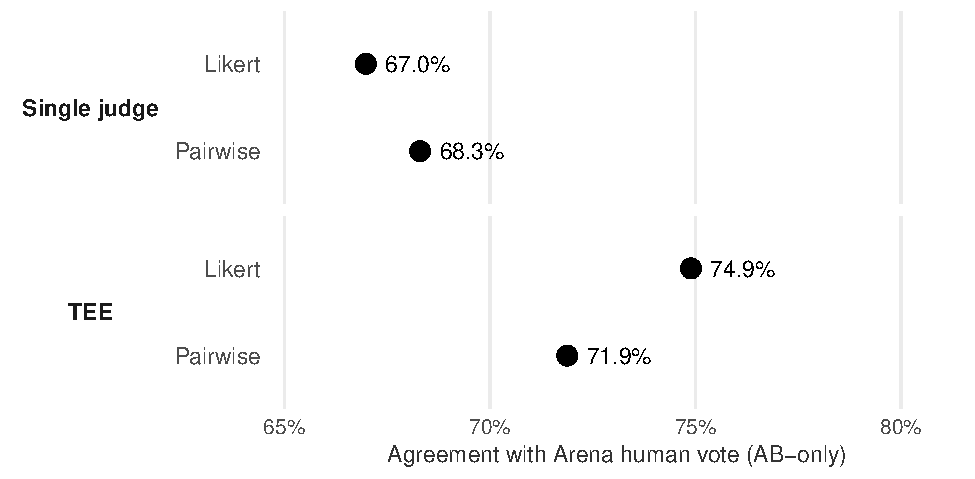
\includegraphics[width=0.9\linewidth]{fig_arena_pipeline_accuracy_dot_pooled.pdf}
\caption{TEE estimation raises agreement with Arena humans by $+7.9$ pp on Likert and $+3.6$ pp on pairwise across 4,676 matches. Each dot is one pipeline's agreement (AB-only, ties excluded).}
\label{fig:arena_accuracy}
\end{figure}

\begin{table}[ht]
\centering
\small
\caption{Agreement with Chatbot Arena human preferences by scoring pipeline and task category. \emph{Overall} counts tied predictions as correct when the human label is also tie. \emph{AB-only} restricts to battles where both sides are decisive.}
\label{tab:arena_agreement}
\begin{tabular}{llrrrr}
\toprule
Category & Pipeline & $N$ & Overall & $N_\text{AB}$ & AB-only \\
\midrule
Creative Writing & Single-judge Likert    &    967 & 0.403 &   343 & 0.668 \\
                 & Single-judge pairwise  & 1,062 & 0.445 &   577 & 0.692 \\
                 & \textbf{TEE Likert}    & 1,064 & 0.424 &   278 & \textbf{0.763} \\
                 & TEE pairwise           & 1,064 & 0.461 &   475 & 0.743 \\
\midrule
Persuasion       & Single-judge Likert    & 1,280 & 0.362 &   327 & 0.618 \\
                 & Single-judge pairwise  & 1,426 & 0.393 &   749 & 0.621 \\
                 & \textbf{TEE Likert}    & 1,428 & 0.391 &   250 & \textbf{0.736} \\
                 & TEE pairwise           & 1,428 & 0.410 &   595 & 0.652 \\
\midrule
Coding           & Single-judge Likert    &    939 & 0.446 &   357 & 0.709 \\
                 & Single-judge pairwise  & 1,078 & 0.421 &   563 & 0.707 \\
                 & \textbf{TEE Likert}    & 1,078 & 0.449 &   351 & \textbf{0.761} \\
                 & TEE pairwise           & 1,078 & 0.441 &   482 & 0.749 \\
\midrule
Factual QA       & Single-judge Likert    & 1,006 & 0.424 &   336 & 0.682 \\
                 & Single-judge pairwise  & 1,105 & 0.474 &   597 & 0.730 \\
                 & \textbf{TEE Likert}    & 1,106 & 0.410 &   292 & \textbf{0.733} \\
                 & TEE pairwise           & 1,106 & 0.453 &   493 & 0.746 \\
\midrule
Pooled           & Single-judge Likert    & 4,192 & 0.405 & 1,363 & 0.670 \\
                 & Single-judge pairwise  & 4,671 & 0.431 & 2,486 & 0.683 \\
                 & \textbf{TEE Likert}    & 4,676 & 0.416 & 1,171 & \textbf{0.749} \\
                 & TEE pairwise           & 4,676 & 0.439 & 2,045 & 0.719 \\
\bottomrule
\end{tabular}
\end{table}

Why does TEE pairwise lift less than TEE Likert? Aggregation mechanics carry most of the gap. TEE Likert averages 30 integer scores per response (one per judge$\times$variant cell) into a fractional mean, so two responses tied at 4 vs.\ 4 by a single judge can split as 4.13 vs.\ 3.87 once 30 cells are pooled. TEE pairwise majority-votes 30 binary verdicts and collapses back to A, B, or tie, discarding the magnitude information that fractional Likert means retain. The pairwise tie ceiling described above magnifies the gap. Roughly one in three Arena battles carry a human tie label, and pairwise judges almost never call ties, so those battles get converted into noisy A/B verdicts that an A/B/tie aggregator cannot rescue. Likert avoids that penalty because two responses can both receive a 3. Single-judge pairwise also starts from a higher base. Its forced-choice format sidesteps integer quantization, central tendency, and scale anchoring, putting it closer to the Arena inter-rater ceiling and leaving less headroom for aggregation to recover.

A D-study fit on the dev split predicts the test-split lifts. For each category, we fit the lmer formula
\begin{verbatim}
score ~ (1|battle_response) + (1|variant_id) + (1|judge_model)
       + (1|battle_response:variant_id)
       + (1|battle_response:judge_model)
       + (1|variant_id:judge_model)
\end{verbatim}
on the dev split's Likert scores, then use the D-study to project per-response score SE under both a single-judge single-variant design ($V{=}1, M{=}1$) and the TEE pipeline ($V{=}5, M{=}3$). The fractional SE reductions across the four categories range 0.53 to 0.59, and the corresponding observed Likert agreement lifts on the test split range $+5.1$ to $+11.8$ pp. The two correlate at Spearman $\rho = 0.80$ (Figure~\ref{fig:arena_dstudy_vs_observed}). Persuasion has both the largest projected variance-reduction headroom and the largest observed lift.

\begin{figure}[ht]
\centering
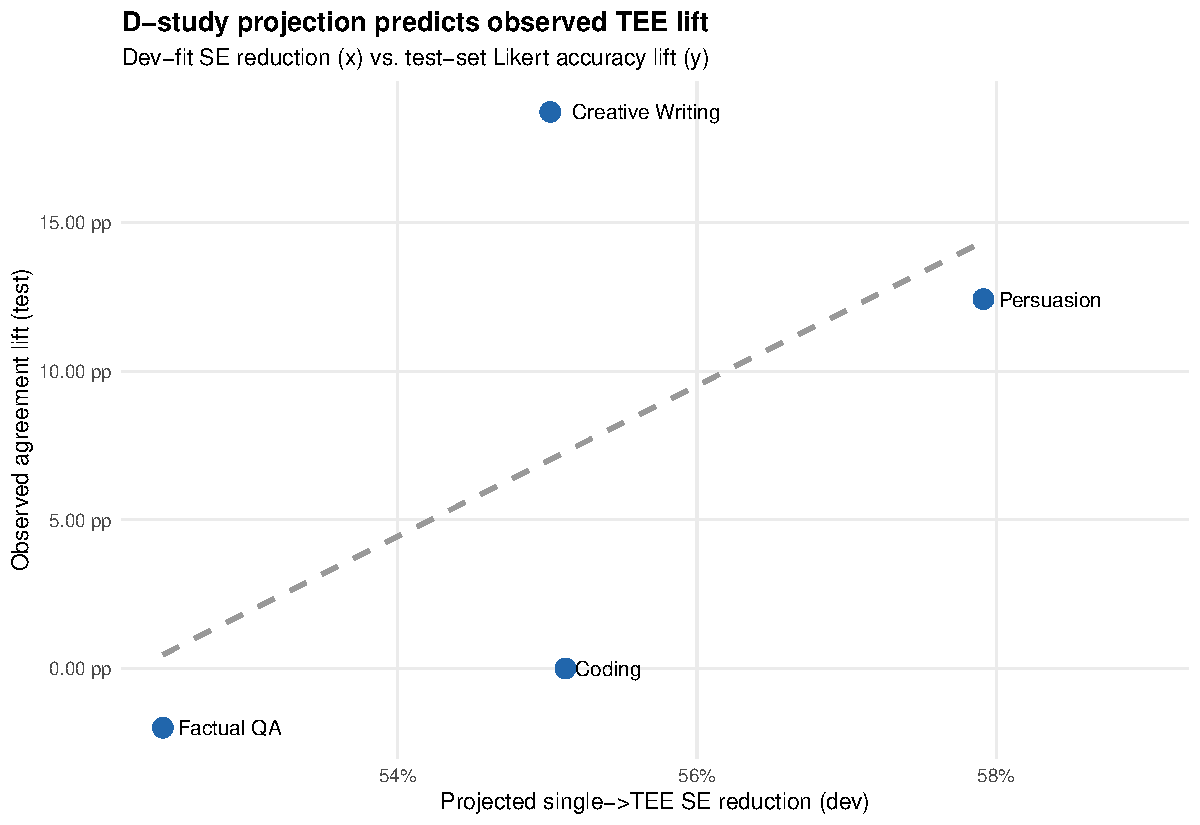
\includegraphics[width=0.85\textwidth]{fig_arena_dstudy_vs_observed.pdf}
\caption{Per-category D-study projection (dev split, x-axis) vs.\ observed Likert agreement lift (test split, y-axis). Spearman $\rho = 0.80$ across the four category points.}
\label{fig:arena_dstudy_vs_observed}
\end{figure}

At the pooled level, AB-only agreement rises from 68.3\% under single-judge pairwise to 71.9\% under TEE pairwise ($+$3.6 pp), smaller than the $+$7.9 pp Likert lift but no longer flat. The simulation in Section~\ref{si:scoring_recovery} confirms the broader pattern that Likert degrades under compression and anchoring pathologies where pairwise BT is invariant, but the present Arena dataset adds a separate calibration headwind that the simulation does not model.

Three caveats apply. First, the variance decomposition is coarser than the framework's main demonstrations because we did not vary temperature or include replications per cell, so the lmer Residual term pools the within-cell replicate noise ($\sigma^2_\rho$) with cell-level idiosyncrasy ($\sigma^2_\epsilon$). A follow-up run with three replications at temperature 1.0 on the same battles would resolve this at roughly double the API cost, and the agreement-rate headline would not change either way. Second, the LLM task categorizer has a nonzero error rate: we spot-checked 50 battles manually and found the label matched a human assessment in 44 of 50 cases (88\%). Categorical mis-tagging attenuates per-category contrasts but should not flip the subjective-vs-objective pattern. Third, roughly 20\% of Arena battles carry a tie label (including \texttt{tie (bothbad)}). The AB-only metric restricts to battles where both the human winner and the pipeline prediction are decisive. The Overall metric in Table~\ref{tab:arena_agreement} counts predicted-tie-matched-to-human-tie as correct. Both metrics support the conclusion that subjective tasks benefit most from TEE.

\subsection{Variance-coverage diagnostics}

Two further variance checks complement the per-battle agreement results. The first is a CI coverage check on the scoring-family mean at the per-battle level. The second is a bootstrap SE check on each model's BT strength at the leaderboard level. Together they probe the naive-vs-TEE gap at two levels of aggregation.

Treat the full Arena Likert factorial as a population of $4,676 \times 5 \times 3 = 70,140$ cells (battles $\times$ variants $\times$ judges). Each cell has a binary outcome $\mathtt{agree} \in \{0, 1\}$ that records whether the single-cell Likert prediction (the sign of the response-pair score difference, with a 0.5 tolerance) matches the Arena human winner. The grand mean across all cells is $p^* = 0.389$, which is the scoring-family accuracy a practitioner implicitly claims to estimate by reporting ``pipeline accuracy.''

From each of $K = 300$ Monte Carlo draws at $n_b \in \{100, 250, 500, 1,000, 2,000\}$ battles, two analysts produce a CI for $p^*$. The naive analyst picks one $(v, j)$ combo uniformly at random and reports $\hat{p} \pm 1.96 \cdot \sqrt{\hat{p}(1 - \hat{p}) / n_b}$. The TEE analyst uses all 15 cells on the same battles, fits $\mathtt{agree} \sim 1 + (1|\mathtt{battle}) + (1|\mathtt{variant}) + (1|\mathtt{judge})$, and reports the Wald CI on the intercept. Figure~\ref{si:arena_coverage} plots coverage and half-width across $n_b$.

Naive coverage falls from $0.93$ at $n_b = 100$ to $0.78$ at $n_b = 2,000$. The binomial SE shrinks below the floor set by between-variant and between-judge variance, so the naive interval tightens around a single cell's mean with no reason to sit near $p^*$. TEE coverage holds at $0.95$ or above throughout, slightly conservative because REML estimates of $\sigma^2_V$ and $\sigma^2_J$ are noisy at $V = 5$ and $J = 3$. In practical terms, a practitioner who reports ``pipeline accuracy $= \hat{p} \pm 1$\,pp'' from $2,000$ battles under a single judge and variant has about 22\% odds that the scoring-family truth sits outside their stated $95\%$ band. The mis-specification lives in the SE, so adding battles only widens the gap. Shrinking the interval further worsens the under-coverage.

\begin{figure}[ht]
\centering
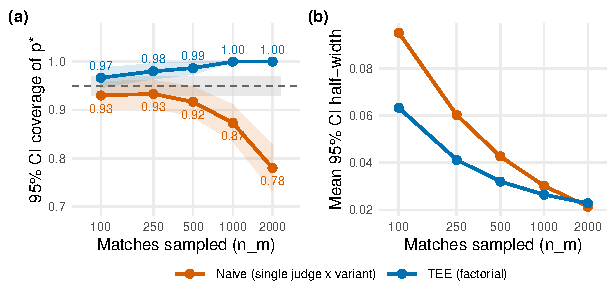
\includegraphics[width=0.78\textwidth]{fig_arena_coverage.pdf}
\caption{Naive (single judge $\times$ variant, binomial Wald) vs.\ TEE (factorial, crossed random-effects Wald) 95\% CI coverage and half-width for the scoring-family mean $p^* = 0.389$, across $K = 300$ Monte Carlo draws per $n_b$. Top: naive coverage degrades as $n_b$ grows because binomial SE shrinks past the between-cell variance floor. TEE coverage holds at or above nominal. Bottom: TEE half-width bottoms out at the $\sigma^2_V / V + \sigma^2_J / J$ floor while naive keeps shrinking. Ribbon: Monte Carlo $\pm 1.96$ SE.}
\label{si:arena_coverage}
\end{figure}

The same mechanism shows up at the leaderboard level. Pipeline-vs-pipeline rank correlations against the same-sample human Bradley-Terry leaderboard \citep{bradley1952rank} are not statistically distinguishable at $n = 55$ models, with Spearman $\rho = 0.86$ - $0.91$ across the four pipelines and all Williams' paired-correlation tests $p > 0.2$. The gap appears instead in the bootstrap SE on each model's BT strength.

For each pipeline, we compare two bootstrap SEs for every model's BT $\log \pi_m$. The naive bootstrap resamples the $4,676$ battles with replacement while keeping each battle's pipeline prediction fixed. The TEE-aware bootstrap also resamples the cell design. For the single-cell pipelines, each TEE-aware rep draws one fresh (judge, variant) cell (or (judge, variant, order) cell for pairwise) uniformly from the $15$ Likert or $30$ pairwise options and applies it to all battles in that rep, this simulates what a researcher who picked a different pipeline configuration would have reported. For the TEE pipelines, each rep resamples the $15$ (Likert) or $30$ (pairwise) cells with replacement per battle and re-aggregates the prediction, this captures the uncertainty from treating the observed variant and judge sets as exchangeable.

Figure~\ref{fig:arena_bt_bootstrap_se} shows the result. For the single-cell pipelines, the TEE-aware SE exceeds the naive SE by a median factor of $1.46$ (Likert) and $3.50$ (pairwise). The naive bootstrap under-reports each model's log-$\pi$ uncertainty by $32\%$ to $72\%$. For the TEE pipelines, the median ratio is $1.01$ (Likert) and $1.08$ (pairwise), confirming negligible change. Cell-level noise averages out across the 15 or 30 within-battle cells, so the BT fit is stable whether the cell set is held fixed or resampled. The per-battle coverage study (Figure~\ref{si:arena_coverage}) and this BT-level bootstrap point to the same mechanism at two levels of aggregation. Cell variance propagates directly into claims that aggregate over a single cell per battle (the naive pipelines) and averages out in proportion to the number of cells aggregated over (the TEE pipelines).

\begin{figure}[ht]
\centering
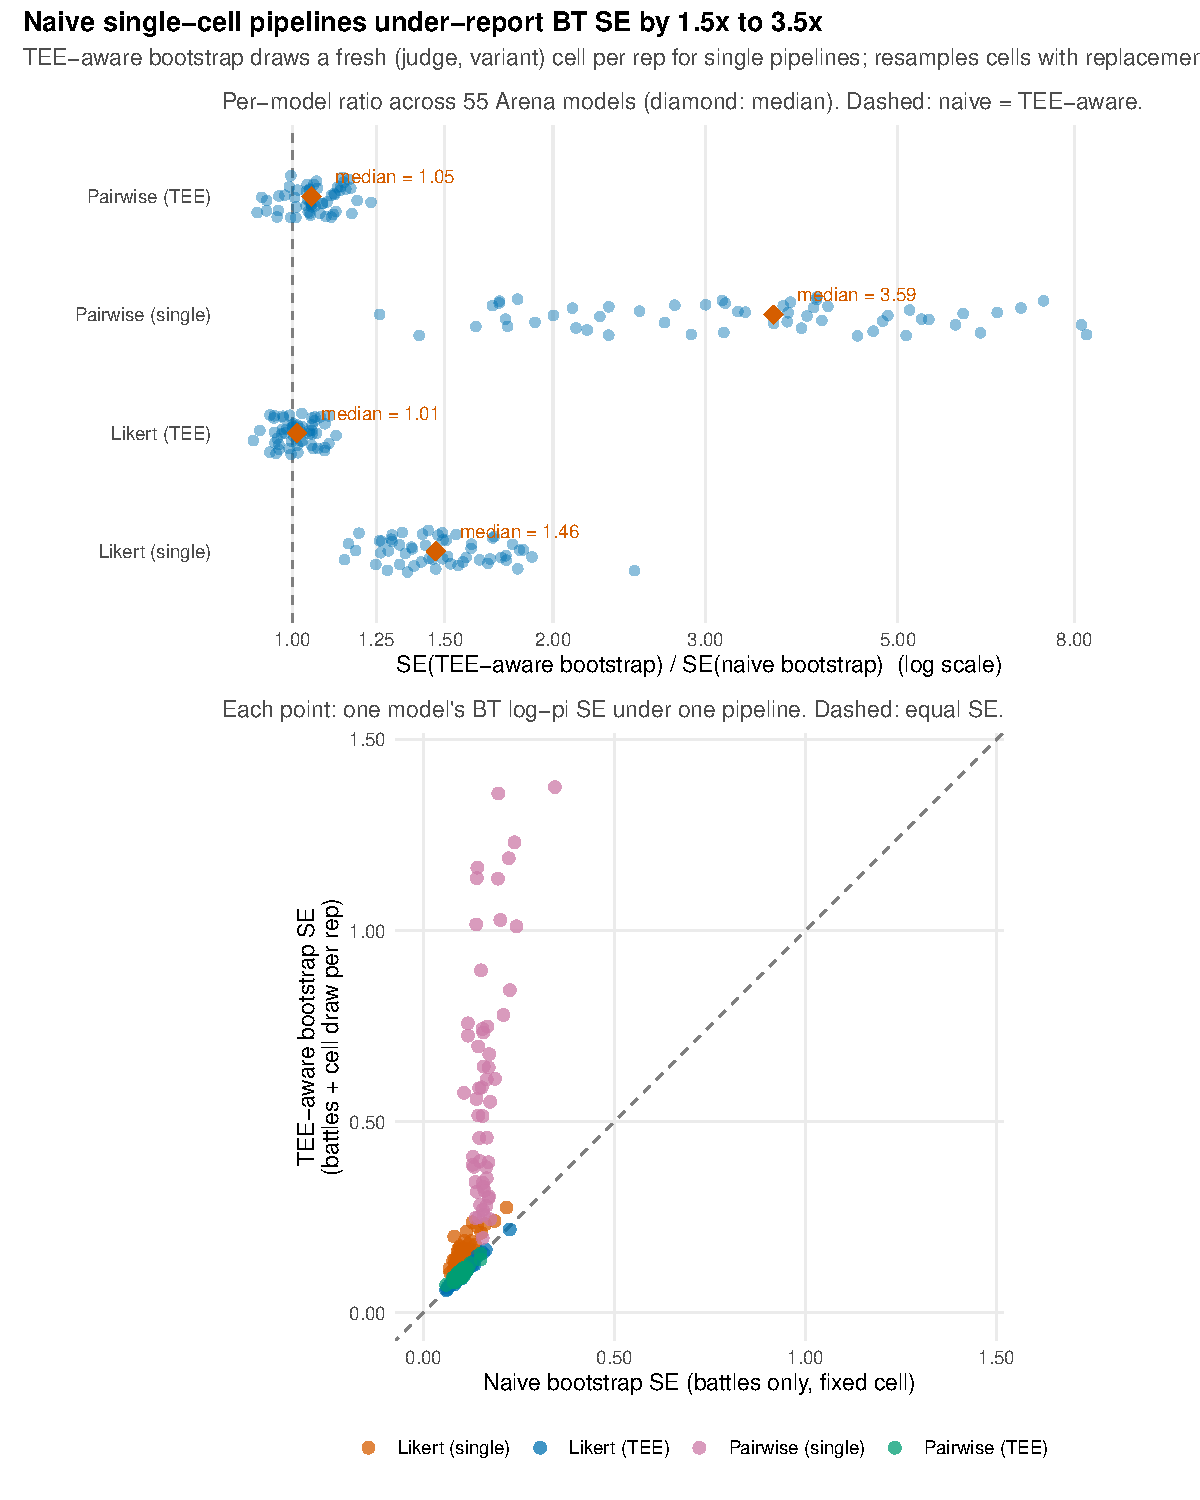
\includegraphics[width=0.85\textwidth]{fig_arena_bt_bootstrap_se.pdf}
\caption{Bootstrap SE for per-model BT $\log \pi_m$ under each of the four pipelines ($N = 300$ reps, $55$ models). Top: ratio of TEE-aware to naive bootstrap SE per model, log-scaled x-axis. Diamond is the per-pipeline median. Bottom: scatter of naive vs.\ TEE-aware SE. Dashed line is equality. Single-cell pipelines cluster above the diagonal (naive under-estimates). TEE pipelines cluster on the diagonal (cell variance is absorbed by aggregation).}
\label{fig:arena_bt_bootstrap_se}
\end{figure}


\end{document}
